\documentclass[17pt,a4paper,twoside]{extbook}




\usepackage[left=1in,right=1in]{geometry}
\usepackage{float}
\usepackage{enumitem}
\usepackage{fancyhdr}
\usepackage{pifont}
\usepackage{commath}
\usepackage{mathtools}
\usepackage[scr]{rsfso}
\usepackage[makeroom]{cancel}
\usepackage{bm}
\usepackage{fancybox,framed}
\usepackage{stackengine}
\usepackage{amssymb,amsmath}
\usepackage{amsthm}
%\usepackage{unicode-math}
\usepackage{esint}
%\usepackage{pxfonts}
\usepackage[overload]{empheq}
\usepackage{cases} 
\usepackage{accents} 
\usepackage[symbol]{footmisc}
\usepackage{cancel}
\usepackage{wrapfig}
\usepackage{graphicx}
\usepackage{subfigure}
\usepackage{xcolor}
\graphicspath{ {figures/} }
\usepackage[titletoc]{appendix}
\usepackage{tikz}
\usetikzlibrary{patterns,patterns.meta}
\usetikzlibrary {arrows.meta}
\usetikzlibrary{angles,quotes, calc}
\usetikzlibrary{decorations.pathreplacing,decorations.markings}
\usetikzlibrary {shapes.geometric}
\usepackage{tikz-3dplot}
\usepackage{pgfplots}
\pgfplotsset{width=10cm,compat=1.9}

\pgfdeclarepattern{
  name=hatch,
  parameters={\hatchsize,\hatchangle,\hatchlinewidth},
  bottom left={\pgfpoint{-.1pt}{-.1pt}},
  top right={\pgfpoint{\hatchsize+.1pt}{\hatchsize+.1pt}},
  tile size={\pgfpoint{\hatchsize}{\hatchsize}},
  tile transformation={\pgftransformrotate{\hatchangle}},
  code={
    \pgfsetlinewidth{\hatchlinewidth}
    \pgfpathmoveto{\pgfpoint{-.1pt}{-.1pt}}
    \pgfpathlineto{\pgfpoint{\hatchsize+.1pt}{\hatchsize+.1pt}}
    \pgfpathmoveto{\pgfpoint{-.1pt}{\hatchsize+.1pt}}
    \pgfpathlineto{\pgfpoint{\hatchsize+.1pt}{-.1pt}}
    \pgfusepath{stroke}
  }
}

\tikzset{
  hatch size/.store in=\hatchsize,
  hatch angle/.store in=\hatchangle,
  hatch line width/.store in=\hatchlinewidth,
  hatch size=5pt,
  hatch angle=0pt,
  hatch line width=.5pt,
}

\tikzset{
    tangent/.style={
        decoration={
            markings,% switch on markings
            mark=
                at position #1
                with
                {
                    \coordinate (tangent point-\pgfkeysvalueof{/pgf/decoration/mark info/sequence number}) at (0pt,0pt);
                    \coordinate (tangent unit vector-\pgfkeysvalueof{/pgf/decoration/mark info/sequence number}) at (1,0pt);
                    \coordinate (tangent orthogonal unit vector-\pgfkeysvalueof{/pgf/decoration/mark info/sequence number}) at (0pt,1);
                }
        },
        postaction=decorate
    },
    use tangent/.style={
        shift=(tangent point-#1),
        x=(tangent unit vector-#1),
        y=(tangent orthogonal unit vector-#1)
    },
    use tangent/.default=1
}
\tikzset{->-/.style={decoration={
  markings,
  mark=at position #1 with {\arrow{Stealth}}},postaction={decorate}}}


\tikzset{
    partial ellipse/.style args={#1:#2:#3}{
        insert path={+ (#1:#3) arc (#1:#2:#3)}
    }
}


\newcommand*\circled[1]{\tikz[baseline=(char.base)]{
            \node[shape=circle,draw,inner sep=2pt] (char) {#1};}}
\usepackage{pdfpages}

\newcommand{\q}[1]{``#1''}


\renewcommand{\thefootnote}{\fnsymbol{footnote}}






\theoremstyle{definition}
\newtheorem{definition}{Definition}[section]
\newtheorem*{example}{Example}
\newtheorem*{exercise}{Exercise}
\newtheorem*{solution}{Solution}
\newtheorem*{notation}{Notation}
\newtheorem*{note}{Note}
\newtheorem*{remark}{Remark}
\newtheorem*{discussion}{Discussion}
\newtheorem*{conclusion}{Conclusion}
%\newtheorem*{claimproof}{Proof of claim \theclaim}
%\newtheorem*{theoremproof}{Proof of theorem \thetheorem}






\theoremstyle{plain}
\newtheorem{theorem}{Theorem}[section]
\newtheorem{lemma}{Lemma}[section]
\newtheorem{claim}{Claim}[section]
\newtheorem{axiom}{Axiom}[section]



%\usepackage[thmmarks]{ntheorem}


%\theorembodyfont{\normalfont}
%\newtheorem{definition}{Definition}[section]
%\theoremstyle{plain}
%\theorembodyfont{\normalfont}
%\newtheorem{example}{Example}
%\theoremstyle{nonumberplain}
%\newtheorem{notation}{Notation}
%
%\theorembodyfont{\itshape}
%\theoremstyle{plain}
%\newtheorem{theorem}{Theorem}
%\newtheorem{lemma}[theorem]{Lemma}
%
%\newtheorem{claim}{Claim}[theorem]
%\theoremstyle{nonumberplain}
%\theoremsymbol{\ensuremath{\Box}}
%\newtheorem{proof}{Proof}
%\theoremsymbol{\ensuremath{\blacksquare}} 
%\newtheorem{claimproof}{Proof of claim \theclaim}

% argumented matrix
\makeatletter
\renewcommand*\env@matrix[1][*\c@MaxMatrixCols c]{%
  \hskip -\arraycolsep
  \let\@ifnextchar\new@ifnextchar
  \array{#1}}
\makeatother
%

% volume
\makeatletter
\DeclareRobustCommand{\volume}{\text{\volumedash}V}
\newcommand{\volumedash}{%
  \makebox[0pt][l]{%
    \ooalign{\hfil\hphantom{$\m@th V$}\hfil\cr\kern0.08em--\hfil\cr}%
  }%
}
%
\makeatother





\usepackage{hyperref}
\hypersetup{hidelinks,
	colorlinks=true,
	allcolors=black,
	pdfstartview=Fit,
	breaklinks=true
}

%------------Command----------------------------------------

\newcommand{\vc}[3]{\overset{#2}{\underset{#3}{#1}}}

%--------------tensor form---------------------
\stackMath
\newcommand\tenq[2][1]{%
 \def\useanchorwidth{T}%
  \ifnum#1>1%
    \stackunder[0pt]{\tenq[\numexpr#1-1\relax]{#2}}{\scriptscriptstyle\sim}%
  \else%
    \stackunder[1pt]{#2}{\scriptscriptstyle\sim}%
  \fi%
}

%-----------------------------------------

\DeclareMathOperator\erf{erf}
\DeclareMathOperator\erfc{erfc}

\DeclareMathOperator\Arg{Arg}
\DeclareMathOperator\Log{Log}

\DeclareMathOperator\arcsec{arcsec}
\DeclareMathOperator\arccot{arccot}
\DeclareMathOperator\arccsc{arccsc}
\DeclareMathOperator\tr{tr}

\def\Res{\mathop{\text{Res}}\limits}

\setlength{\headheight}{63.0pt}




\title{%
Ideal-Fluid Flow}

\author{Prof. Tzuyin Wu}
\date{Jan 26, 2024}

\begin{document}

\frontmatter

\maketitle


\pagenumbering{Roman}
%\pagestyle{empty}
%\pagenumbering{gobble}
\pagestyle{fancy}
\fancyhf{}
\fancyhead[C]{\textbf{\leftmark}}
\fancyfoot[C,CO]{\thepage}
\tableofcontents

%\listoffigures

%\newpage
%\pagestyle{empty}

\newpage
\mainmatter
\pagenumbering{arabic}
\pagestyle{fancy}
%\setcounter{page}{1}
\fancyhf{}
\fancyhead[CO]{\textbf{\leftmark}}
\fancyhead[CE]{\textbf{\rightmark}}
%\fancyhead[C]{\textbf{\leftmark}}
%\fancyhead[C]{\textbf{\rightmark}}
\fancyfoot[C,CO]{\thepage}
\fancyfoot[L,L]{\footnotesize Prof. Tzuyin Wu}
\renewcommand{\footrulewidth}{1pt}

\raggedright




% !TeX root = ../Ideal-Fluid Flow.tex
\chapter{Introduction}
\section{Ideal-Fluid}
\begin{definition}\mbox{}\\
\[
\textrm{Ideal-fluid}
\left\{
\begin{aligned}
&\textrm{Inviscid }(\mu = 0)\\
&\textrm{Incompressible flow }(\rho=\textrm{constant})
\end{aligned}
\textrm{fluid}
\right.
\]
The flow field generated by such flow $\Longrightarrow$ \emph{Ideal flow}
\end{definition}
\begin{note}\mbox{}\\
More commonly, ideal flow deals with flows which are \emph{inviscid} $(\mu=0)$, \emph{incompressible} $(\rho=\textrm{constant})$, and also \emph{irrotational} $(\nabla\times\mathbf{u}=\mathbf{0})$. Such flows are called \emph{Potential Flows}.
\end{note}
\begin{itemize}
\item Justifications:\\
For real fluids, more and less, $\mu\neq 0$, $\rho\neq$constant.
\begin{enumerate}[label = <\roman*>]
\item Cases when flows can be treated as \emph{inviscid}. Air and water have negligible viscosity. $(\nu = \mu/\rho\sim\mathcal{O}(10^{-5}\sim 10^{-6})\textrm{m\textsuperscript{2}/s})$\label{1-1-i}
\begin{enumerate}[label = \protect\circled{\arabic*}]
\item near a solid body (e.g. boundary layer)
\begin{figure}[H]
\centering
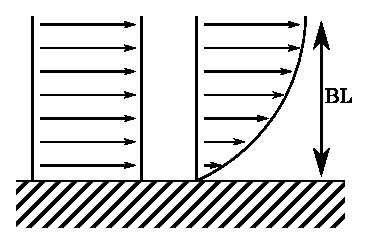
\includegraphics[scale=1.0]{figure/chapter1/1-1-1.eps}
%\caption{Scheme of blowing/suction flow}
%\label{Scheme of blowing/suction flow}
\end{figure}
\item wake
\begin{figure}[H]
\centering
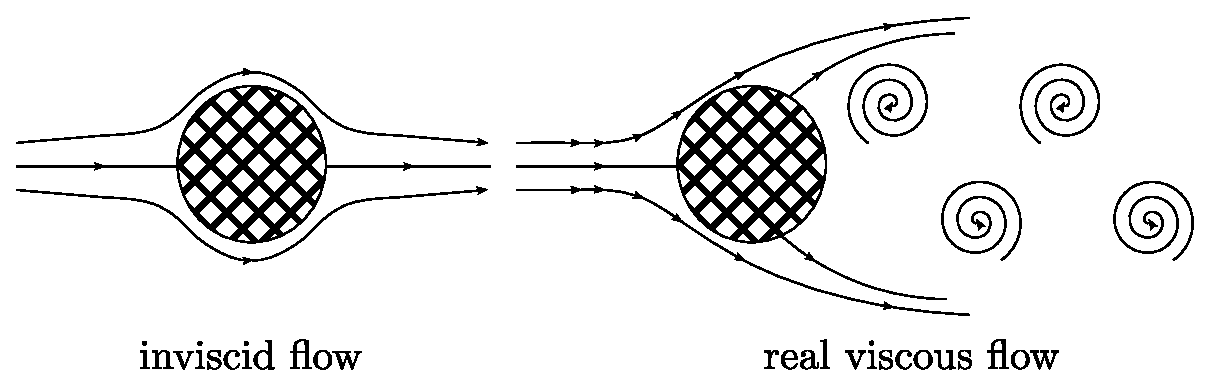
\includegraphics[scale=0.7]{figure/chapter1/1-1-2.eps}
%\caption{Scheme of blowing/suction flow}
%\label{Scheme of blowing/suction flow}
\end{figure}
\item fluid-fluid interface, shock...
\end{enumerate}
In general, viscosity effect can be neglected if $Re = UL/\nu\ll 1$
\item Cases when flows can be treated as \emph{incompressible}.\label{1-1-ii}
\begin{enumerate}[label = (\alph*)]
\item Almost in all cases, the \emph{liquid} can be taken as \emph{incompressible}.
\item For \emph{gases}, we can neglect their compressibility if the variation in density $\Delta p/\rho$ in the flow is $<5\%$.
\begin{enumerate}[label = \protect\circled{\arabic*}]
\item in the case where variation in density is largely due to \emph{pressure change} from Bernoulli's equation.\label{1.1-1}
\[
\frac{d(v^2/2)}{ds} = -\frac{1}{\rho}\frac{dp}{ds}
\]
\begin{equation}
\Longrightarrow\frac{\Delta p}{\rho}\sim\frac{(\Delta v)^2}{2}\sim\frac{U_\infty^2}{2}
\label{eq: 1-1}
\end{equation}
The sound speed ``$a$'' is defined:
\begin{align*}
a = \sqrt{\left.\frac{\partial p}{\partial \rho}\right|_s} = \sqrt{\gamma RT},&& \gamma = \frac{c_p}{c_v}
\end{align*}
\begin{align*}
\therefore a^2 = \gamma RT = \gamma\frac{p}{\rho}, && \boxed{M_\infty = \frac{U_\infty}{a}}\textrm{ (Mach number)}
\end{align*}
\begin{equation}
\Longrightarrow \frac{U_\infty^2}{p/\rho} = \gamma M_\infty^2
\label{eq: 1-2}
\end{equation}
substitute \eqref{eq: 1-2} into \eqref{eq: 1-1}
\begin{equation}
\Longrightarrow \frac{\Delta p}{p}\sim \frac{\gamma}{2}M_\infty^2
\label{eq: 1-3}
\end{equation}
use $p = \rho RT$, take $T\approx$constant,
\begin{equation}
\Longrightarrow\frac{\Delta p}{p}\sim\frac{\Delta\rho}{rho}\Longrightarrow\boxed{\frac{\Delta\rho}{\rho}\sim\frac{\gamma}{2}M_\infty^2}
\label{eq: 1-4}
\end{equation}
For most gases, $\gamma\approx 1$, hence $\Delta\rho/\rho <5\%$ if $\underline{M_\infty <0.3}$.
\item in the case where variation in density is largely due to \emph{temperature change}\label{1.1-2}\\
Assume \emph{adiabatic process}
\begin{align*}
dh = c_pdT, && h + \frac{v^2}{2} = \textrm{constant}
\end{align*}
\begin{equation}
\Longrightarrow\Delta T = \frac{\left(\Delta v\right)^2}{2c_p}\Longrightarrow T_\infty = \frac{U_\infty^2}{2c_p}
\label{eq: 1-5}
\end{equation}
also
\begin{align*}
a^2 = \gamma R T_\infty, && c_p = \frac{\gamma R}{\gamma - 1}
\end{align*}
hence 
\begin{equation}
\eqref{eq: 1-5}\Longrightarrow \frac{\Delta T}{T_\infty} = \frac{\gamma -1}{2}M_\infty^2
\label{eq: 1-6}
\end{equation}
For reversible, adiabatic process,
\begin{align*}
p\rho^{-\gamma} = c && \text{ or }pv^\gamma = c && \text{ or }T\rho^{1-\gamma} = c
\end{align*}
\[
\therefore\frac{\Delta T}{T_\infty}\sim\left(\gamma-1\right)\frac{\Delta\rho}{\rho_\infty}
\]
hence
\begin{equation}
\eqref{eq: 1-6}\Longrightarrow
\boxed{
\frac{\Delta\rho}{\rho_\infty}\sim\frac{M_\infty^2}{2}
}
\label{eq: 1-7}
\end{equation}
\begin{align*}
\frac{\Delta\rho}{\rho_\infty}< 5\% \text{ if }\boxed{M_\infty< 0.3}
\end{align*}
\end{enumerate}
\end{enumerate}
\end{enumerate}
$
\left.
\begin{aligned}
&\ref{1.1-1} \\
&\ref{1.1-2}
\end{aligned}
\right\}
\Longrightarrow$
In general, the flow can be treated as incompressible if $M_\infty <0.3\%$.

Combine \ref{1-1-i} and \ref{1-1-ii}, the flow can be treated as an Ideal flow if 
$\left\{
\begin{aligned}
&Re \gg 1\\
&M < 0
\end{aligned}\right.$\\
except region
$\left\{
\begin{aligned}
&\text{Boundary layer} (BL)\\
&\text{Wake} \\
&\text{shock}
\end{aligned}\right.
$
\item Applications: 
\begin{enumerate}[label = \protect\circled{\arabic*}]
\item Hydraulic (e.g. Bernoulli's equation) \\
\item Surface waves
\item Aerodynamics (e.g. Thin-airfoil Theory)
\end{enumerate}
\end{itemize}

\chapter{Equations for the Motion of an Ideal-Fluid}
\section{Method of Analysis}
Two descriptions methods for fluid motion
\begin{enumerate}[label = (\arabic*)]
\item Lagrangian description\\
--tracing the motion of each fluid element (control-mass approach), i.e., $\mathbf{x} = \mathbf{x}(\boldsymbol{\xi},t)$ where $\boldsymbol{\xi}$ specifies the initial position of the fluid element, then
\begin{align*}
\mathbf{v}\equiv\left(\frac{\partial\mathbf{x}}{\partial t}\right)_{\boldsymbol{\xi}}&&\text{ and }&&\mathbf{a}\equiv\left(\frac{\partial^2\mathbf{x}}{\partial t^2}\right)_{\boldsymbol{\xi}}&&\text{etc.}
\end{align*}
\item Eulerian description \\
--recording fluid motion at each fixed location (field description, control-volume approach), i.e., $\mathbf{v} = \mathbf{v}(\mathbf{x},t)$ where $\mathbf{x}$ are fixed spatial coordinates.
\[
\therefore\mathbf{v}\neq \frac{\partial\mathbf{x}}{\partial t}.
\]
\end{enumerate}
Analysis can be classified as:
\begin{enumerate}[label = \protect\circled{\arabic*}]
\item Integral analysis-- Conservation laws being applied to a fixed region.
\item Differential analysis-- Conservation laws being applied, in a limiting case, to a point. This requires flow properties to be differentiable. 
\end{enumerate}

\section{Reynolds Transport Theorem (RTT)}
Laws of Mechanics are applied to a control-mass system (Lagrangian description). RTT converts the system analysis to an equivalent expression in control-volume approach (Eulerian description).
\begin{itemize}
\item Substantial derivative (time rate of change of properties following fluid motion)\\
Let $B(\mathbf{x},t)$ be a scalar (or vector) function, then 
%----------------------
\begin{minipage}{0.4\textwidth}
\begin{align*}
dB &= d\mathbf{x}\cdot\nabla B + \frac{\partial B}{\partial t}dt \\
\therefore
\frac{dB}{dt} &= \mathbf{v}\cdot B + \frac{\partial B}{\partial t}
\end{align*}
or 
\begin{equation}
\underbrace{\frac{DB}{Dt}}_
{
\begin{subarray}{c}
  \text{Lagrangian}\\
  \text{derivative}
\end{subarray}
}= \underbrace{\mathbf{v}\cdot\nabla B + \frac{\partial B}{\partial t}}_
{
\begin{subarray}{c}
  \text{equivalent}\\
  \text{Eulerian expression}
\end{subarray}
}
\label{eq: 2-1}
\end{equation}
\end{minipage} \hfill
\begin{minipage}{0.4\textwidth}
\begin{figure}[H]
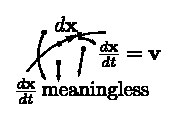
\includegraphics[scale=1.8]{figure/chapter2/2-1-1.eps}
%\caption{\label{fig:blue_rectangle} Rectangle}
\end{figure}
\end{minipage}
%----------------------
\item RTT \\
Let $\volume(t)$ be a closed region moving with the fluid (i.e. material volume) with boundary surface denoted by $S(t)$ and let $B(\mathbf{x},t)\footnotemark$ denote any \emph{intensive} property of the fluid field\footnotetext{could be scalar or vector function}, then

\begin{figure}[H]
\centering
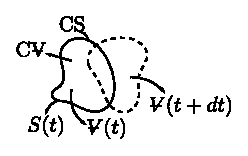
\includegraphics[scale=1.8]{figure/chapter2/2-1-2.eps}
%\caption{Scheme of blowing/suction flow}
%\label{Scheme of blowing/suction flow}
\end{figure}
\begin{subequations}
\label{eq: 2-2}
\begin{flalign}
\frac{D}{Dt}{\oiint \hspace{-23.5pt} \int}_{\volume(t)}\rho B d\volume
&\vc{=}{\footnotemark}{} {\oiint \hspace{-23.5pt} \int}_{\volume(t)}\frac{D\left(\rho B\right)}{Dt}d\volume + \rho B\frac{D\left(d\volume\right)}{Dt} \nonumber \\
&={\oiint \hspace{-23.5pt} \int}_{C\volume} \frac{D\left(\rho B\right)}{Dt}d\volume + \rho B\left(\nabla\cdot\mathbf{v}\right)d\volume \\
&= {\oiint \hspace{-23.5pt} \int}_{C\volume}\left[\frac{\partial\left(\rho B\right)}{\partial t} + \nabla\cdot\left(\rho B \mathbf{v}\right)\right]d\volume \\
&= {\oiint \hspace{-23.5pt} \int}_{C\volume}\frac{\partial\left(\rho B\right)}{\partial t}d\volume + \oiint_{CS}\mathbf{n}\cdot\left(\rho B\mathbf{v}\right)dS
\end{flalign}
\footnotetext{Recall $\displaystyle\nabla\cdot\mathbf{v} = \frac{1}{d\volume}\frac{D\left(d\volume\right)}{Dt}$, then $\displaystyle\frac{D\left(d\volume\right)}{Dt} = \left(\nabla\cdot\mathbf{v}\right)d\volume$}
\end{subequations}
\end{itemize}
\section{Differential Equations for an Ideal-Fluid Motion}
\begin{itemize}
\item Conservation of mass
\[
\frac{D}{Dt}{\oiint \hspace{-23.5pt} \int}_{\volume (t)}\rho d\volume = 0
\]
Apply RTT (set $B\equiv 1$) 
\begin{subequations}
\begin{align}[left = \empheqlbrace\,]
&{\oiint \hspace{-23.5pt} \int}_{C\volume}\frac{\partial\rho}{\partial t} d\volume + \underbrace{\oiint_{CS}\mathbf{n}\cdot\left(\rho \mathbf{v}\right)dS}_
{
\begin{subarray}{c}
  \text{net mass flow rate}\\
  \text{across CS (mass flux)}
\end{subarray}
}
= 0 \\
&{\oiint \hspace{-23.5pt} \int}_{C\volume}\left[\frac{\partial\rho}{\partial t} + \nabla\cdot\left(\rho\mathbf{v}\right)\right]d\volume = 0
\end{align}
\end{subequations}
Since C$\volume$ is \emph{arbitrary}
\begin{subequations}
\begin{align}
\Longrightarrow &\boxed{\frac{\partial\rho}{\partial t} + \nabla\cdot\left(\rho\mathbf{v}\right) = 0}\text{ everywhere} \\
\text{or }&\underbrace{\frac{\partial\rho}{\partial t}+\mathbf{v}\cdot\nabla\rho}_{\displaystyle\equiv\frac{D\rho}{Dt}} + \rho\nabla\cdot\mathbf{v} = 0\nonumber \\
\Longrightarrow & \frac{D\rho}{Dt} + \rho\nabla\cdot\mathbf{v} = 0
\end{align}
\end{subequations}
For an ideal fluid, $\rho =$ constant
\begin{align}
\Longrightarrow \frac{D\rho}{Dt} = 0&&\text{ or }&&\boxed{\nabla\cdot\mathbf{v} = 0}\text{ everywhere}
\end{align}
\item Conservation of Momentum
\begin{equation}
\frac{D}{Dt}{\oiint \hspace{-23.5pt} \int}_{\volume (t)}\rho\mathbf{v}d\volume = \sum\mathbf{F} = {\oiint \hspace{-23.5pt} \int}_{\volume (t)}\mathbf{f_b}d\volume + \oiint_{S(t)}\mathbf{f_s}dS
\tag{$\ast$} \label{eq: 2-*}
\end{equation}
where 
\begin{align*}
\mathbf{f_b}&\colon\text{body force/volume},\mathbf{f_b} = \rho\mathbf{g} \\
\mathbf{f_s}&\colon\text{surface force/area},\mathbf{f_s} = \mathbf{n}\cdot\boldsymbol{\tau}
\end{align*}
\[
\eqref{eq: 2-*}\Longrightarrow
\frac{D}{Dt}{\oiint \hspace{-23.5pt} \int}_{\volume (t)}\rho\mathbf{v}d\volume = {\oiint \hspace{-23.5pt} \int}_{\volume (t)}\rho\mathbf{g}d\volume + \oiint_{S(t)}\mathbf{n}\cdot\boldsymbol{\tau}dS
\]
Apply RTT (set $B=\mathbf{v}$)
\begin{subequations}
\begin{align}[left = \empheqlbrace\,]
&{\oiint \hspace{-23.5pt} \int}_{C\volume}\frac{\partial\left(\rho\mathbf{v}\right)}{\partial t} d\volume + \underbrace{\oiint_{CS}\mathbf{n}\cdot\left(\rho \mathbf{v}\mathbf{v}\right)dS}_
{
\begin{subarray}{c}
  \text{net momentum flux}\\
  \text{across CS}
\end{subarray}
}\nonumber \\
&= {\oiint \hspace{-23.5pt} \int}_{C\volume }\rho\mathbf{g}d\volume + \oiint_{CS}\mathbf{n}\cdot\boldsymbol{\tau}dS \\
&{\oiint \hspace{-23.5pt} \int}_{C\volume}\frac{\partial\left(\rho\mathbf{v}\right)}{\partial t} d\volume + \oiint_{C\volume}\nabla\cdot\left(\rho \mathbf{v}\mathbf{v}\right)d\volume \nonumber\\ 
&= {\oiint \hspace{-23.5pt} \int}_{C\volume }\rho\mathbf{g}d\volume + {\oiint \hspace{-23.5pt} \int}_{C\volume }\nabla\cdot\boldsymbol{\tau}d\volume
\end{align}
\end{subequations}
Since C$\volume$ is \emph{arbitrary}
\begin{subequations}
\begin{align}
\Longrightarrow &\frac{\partial\left(\rho\mathbf{v}\right)}{\partial t} + \nabla\cdot\left(\rho \mathbf{v}\mathbf{v}\right) = \rho\mathbf{g} + \nabla\cdot\boldsymbol{\tau} \\
&\text{Use }\nabla\cdot\left(\rho\mathbf{v}\mathbf{v}\right) = \left[\nabla\cdot\left(\rho\mathbf{v}\right)\right]\mathbf{v} + \rho\mathbf{v}\cdot\left(\nabla\mathbf{v}\right) \nonumber\\
&\text{and apply continuity equation}\nonumber\\
\Longrightarrow &\underbrace{\rho\frac{\partial\mathbf{v}}{\partial t} + \rho \mathbf{v}\cdot\nabla\mathbf{v}}_{\displaystyle =\rho\frac{D\mathbf{v}}{Dt}} = \rho\mathbf{g} + \nabla\cdot\boldsymbol{\tau} \label{eq: 2-7b}
\end{align}
\end{subequations}
For an ideal fluid, $\mu = 0$,
\[
\boldsymbol{\tau} = -p\mathbf{I}\text{ only}
\]
hence \eqref{eq: 2-7b} reduce to
\begin{equation}
\boxed{\rho\frac{D\mathbf{v}}{Dt} = \rho \mathbf{g} - \nabla p}\text{ (Euler equation)}
\label{eq: 2-8}
\end{equation}
\item Conservation of Energy (1\textsuperscript{st} law of thermodynamics)
\begin{multline*}
\frac{D}{Dt}{\oiint \hspace{-23.5pt} \int}_{\volume (t)}\rho\left(e + \frac{v^2}{2}\right)d\volume = \sum\mathbf{F}\cdot\mathbf{v} \\
= {\oiint \hspace{-23.5pt} \int}_{\volume (t)}\mathbf{f_b}\cdot\mathbf{v}d\volume + \oiint_{S(t)}\mathbf{f_s}\cdot\mathbf{v}dS - \oiint_{S(t)}\mathbf{n}\cdot\mathbf{\dot{q}}dS \\
= {\oiint \hspace{-23.5pt} \int}_{\volume (t)}\rho\mathbf{g}\cdot\mathbf{v} d\volume + \oiint_{S(t)}\left(\mathbf{n}\cdot\boldsymbol{\tau}\right)\cdot\mathbf{v}dS + \oiint_{S(t)}\mathbf{n}\cdot\left(k\nabla T\right)dS
\end{multline*}
where 
\begin{align*}
e&\colon\text{internal energy/mass} \\
\frac{v^2}{2}&\colon\text{macro kinetic energy/mass}
\end{align*}
Apply RTT (set $B=e+v^2/2$)
\begin{subequations}
\begin{align}[left = \empheqlbrace\,]
&{\oiint \hspace{-23.5pt} \int}_{C\volume}\frac{\partial}{\partial t}\left[\rho\left(e+\frac{v^2}{2}\right)\right] d\volume \nonumber \\ 
&+ \underbrace{\oiint_{CS}\mathbf{n}\cdot\left[\rho\left(e+\frac{v^2}{2}\right)\right]dS}_
{
\begin{subarray}{c}
  \text{net energy flux}\\
  \text{across CS}
\end{subarray}
}\nonumber \\
&= {\oiint \hspace{-23.5pt} \int}_{C\volume }\rho\mathbf{g}\cdot\mathbf{v} d\volume + \oiint_{CS}\left(\mathbf{n}\cdot\boldsymbol{\tau}\right)\cdot\mathbf{v}dS\nonumber \\
& + \oiint_{CS}\mathbf{n}\cdot\left(k\nabla T\right)dS\\
&{\oiint \hspace{-23.5pt} \int}_{C\volume}\frac{\partial}{\partial t}\left[\rho\left(e+\frac{v^2}{2}\right)\right] d\volume \nonumber \\ 
&+ {\oiint \hspace{-23.5pt} \int}_{C\volume}\nabla\cdot\left[\rho\left(e+\frac{v^2}{2}\right)\right]d\volume\nonumber \\
&= {\oiint \hspace{-23.5pt} \int}_{C\volume }\rho\mathbf{g}\cdot\mathbf{v} d\volume + {\oiint \hspace{-23.5pt} \int}_{C\volume}\nabla\cdot\left(\boldsymbol{\tau}\cdot\mathbf{v}\right)d\volume\nonumber \\
& + {\oiint \hspace{-23.5pt} \int}_{C\volume}\nabla\cdot\left(k\nabla T\right)d\volume
\end{align}
\end{subequations}
Since C$\volume$ is \emph{arbitrary}
\begin{subequations}
\begin{align}
\Longrightarrow &\frac{\partial}{\partial t}\left[\rho\left(e+\frac{v^2}{2}\right)\right] + \nabla\cdot\left[\rho\left(e+\frac{v^2}{2}\right)\right]\nonumber\\ 
&= \rho\mathbf{g}\cdot\mathbf{v} + \nabla\cdot\left(\boldsymbol{\tau}\cdot\mathbf{v}\right)  + \nabla\cdot\left(k\nabla T\right)\\
&\text{Use continuity/momentum equation}\nonumber\\
\Longrightarrow &\rho \frac{D}{Dt}\left[\rho\left(e+\frac{v^2}{2}\right)\right]\nonumber\\ 
&= \rho\mathbf{g}\cdot\mathbf{v} + \nabla\cdot\left(\boldsymbol{\tau}\cdot\mathbf{v}\right)  + \nabla\cdot\left(k\nabla  T\right)\label{eq: 2-10b}
\end{align}
\end{subequations}
For an ideal fluid, 
$
\left\{
\begin{aligned}
\rho = \text{ constant}&\Longrightarrow \nabla\cdot\mathbf{v} = 0 \\
\mu = 0&\Longrightarrow\boldsymbol{\tau} = -p\mathbf{I}
\end{aligned}
\right.
$
hence \eqref{eq: 2-10b} reduce to
\begin{equation}
\rho \frac{D}{Dt}\left[\rho\left(e+\frac{v^2}{2}\right)\right] = \rho\mathbf{g}\cdot\mathbf{v}-\nabla\cdot\left(p\mathbf{v}\right) + \nabla\left(k\nabla T\right)\tag{$\ast$}\label{eq: 2-1-*}
\end{equation}
From momentum equation \eqref{eq: 2-8} perform
\begin{equation}
\mathbf{v}\cdot\left\{\rho\frac{D\mathbf{v}}{Dt} = \rho \mathbf{g} - \nabla p\right\}\tag{$\ast\ast$}\label{eq: 2-1-**}
\end{equation}
notice that
\begin{align*}
\mathbf{v}\cdot\left[\mathbf{v}\cdot\nabla\mathbf{v}\right]
&= \mathbf{v}\cdot\left[\nabla\left(\frac{v^2}{2}\right) - \mathbf{v}\times\underbrace{\left(\nabla\times\mathbf{v}\right)}_{=\boldsymbol{\xi}}\right] \\
&= \mathbf{v}\cdot\nabla\left(\frac{v^2}{2}\right)  - \underbrace{\mathbf{v}\cdot\left(\mathbf{v}\times\boldsymbol{\xi}\right)}_{=0}
\end{align*}
hence \eqref{eq: 2-1-**}
\begin{equation}
\Longrightarrow\rho\frac{ D}{Dt}\left(\frac{v^2}{2}\right) = \rho \mathbf{g}\cdot\mathbf{v} - \mathbf{v}\cdot\nabla p
\label{eq: 2-1-11}
\end{equation}
Subtract \eqref{eq: 2-1-11} from \eqref{eq: 2-1-*}
 \begin{equation}
\Longrightarrow\rho\frac{ De}{Dt} =  - \mathbf{v}\cdot\nabla p + \nabla\cdot\left(k\nabla T\right)
\label{eq: 2-1-12}
\end{equation}
For ideal fluid, $\nabla\cdot\mathbf{v} = 0$ and non-conducting, $k=0$,
\[
\Longrightarrow\boxed{\frac{De}{Dt} = 0}
\]
Thus, don't need energy equation when dealing with ideal flows.
\end{itemize}
\section{Boundary Condition for an Ideal-Fluid Motion}
\begin{itemize}
\item At solid-fluid boundary-- No penetration condition
%----------------------
\begin{minipage}{0.4\textwidth}
\begin{equation}
\boxed{\mathbf{v}\cdot\mathbf{n} = \mathbf{v_s}\cdot\mathbf{n}}
\label{eq: 2-13}
\end{equation}
\end{minipage} \hfill
\begin{minipage}{0.4\textwidth}
\begin{figure}[H]
\centering
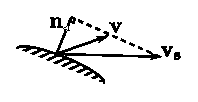
\includegraphics[scale=1.8]{figure/chapter2/2-1-3.eps}
%\caption{\label{fig:blue_rectangle} Rectangle}
\end{figure}
\end{minipage}\\
%----------------------
If body is fixed, $\mathbf{v_s} = \mathbf{0}$
\begin{equation}
\eqref{eq: 2-13}\Longrightarrow\boxed{\mathbf{v}\cdot\mathbf{n} = 0}
\label{eq: 2-14}
\end{equation}
i.e., fluid can only slide on the solid body surface.
\item At fluid-fluid boundary\\
Assume immiscible situation
\begin{enumerate}[label = (\alph*)]
\item Kinematic conditions\\
Let $F(\mathbf{x},t)=0$ represents the instantaneous  position of the interface, then\\
%----------------------
\begin{minipage}{0.2\textwidth}
\begin{align}
&\boxed{\mathbf{v_A}\cdot\mathbf{n} = \mathbf{v_B}\cdot\mathbf{n}}\label{eq: 2-15} \\
&\text{ or }\left(\mathbf{v_A}-\mathbf{v_B}\right)\cdot\underbrace{\nabla F}_{\parallel\mathbf{n}} = 0\nonumber
\end{align}
\end{minipage} \hfill
\begin{minipage}{0.4\textwidth}
\begin{figure}[H]
\centering
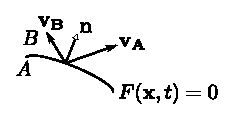
\includegraphics[scale=1.8]{figure/chapter2/2-1-4.eps}
%\caption{\label{fig:blue_rectangle} Rectangle}
\end{figure}
\end{minipage}\\
%----------------------
but the tangential components may be different across the interface $\Longrightarrow$ surface of tangential discontinuity.\\
e.g. 
\begin{figure}[H]
\centering
\subfigure[Ideal-Fluid flow]
{
%\label{3-7-Plot of frequency response in amplitude}
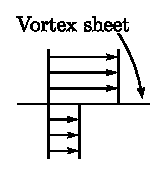
\includegraphics[scale=1.5]{figure/chapter2/2-1-5-a.eps}
}
\centering
\subfigure[Real flow]
{
%\label{3-7-Plot of frequency response in phase}
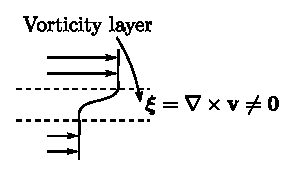
\includegraphics[scale=1.5]{figure/chapter2/2-1-5-b.eps}
}
%\caption{Plot of frequency response}
\end{figure}
\item Dynamic condition\\
%----------------------
\begin{minipage}{0.4\textwidth}
\begin{figure}[H]
\centering
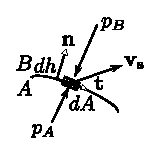
\includegraphics[scale=1.8]{figure/chapter2/2-1-6.eps}
%\caption{\label{fig:blue_rectangle} Rectangle}
\end{figure}
\end{minipage} \hfill
\begin{minipage}{0.4\textwidth}
Take a small element moving with the interface $dhdA$ over a segment of the interface, the force balance equation in the $\mathbf{n}-$direction
\end{minipage}\\
%----------------------
\[
f_{bn}dAdh + \left(p_A-p_B\right)dA - \underbrace{\sum a_{\text{rel},n}\left(\rho dA dh\right)}_{\text{Apparent force terms}} = 0
\]
\begin{equation}
\text{As } dh\to 0\Longrightarrow\boxed{p_A=p_B}
\label{eq: 2-16}
\end{equation}
\end{enumerate}
\end{itemize}
\chapter{Kinematic and Dynamics of Ideal-Fluid Motion}
\section{Kinematic}
\subsection{Streamlines and Vorticity Lines}
\begin{itemize}
\item Streamlines: A curve that is everywhere tangent to the (instantaneous) local velocity vectors.
\item Vorticity lines: A curve that is everywhere tangent to the (instantaneous) local vorticity vectors.
\begin{figure}[H]
\centering
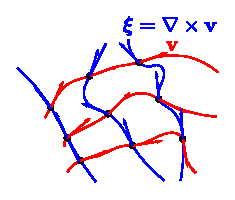
\includegraphics[scale=1.8]{figure/chapter3/3-1-1.eps}
%\caption{\label{fig:blue_rectangle} Rectangle}
\end{figure}
\item Equation of streamline\\
%----------------------
\begin{minipage}{0.4\textwidth}
\begin{equation}
\frac{dx}{u} = \frac{dy}{v} = \frac{dz}{w}
\label{eq: 3-1-1}
\end{equation}
Similarly, for vorticity line
\begin{equation}
\frac{dx}{\xi_x} = \frac{dy}{\xi_y} = \frac{dz}{\xi_z}
\label{eq: 3-1-2}
\end{equation}
\end{minipage} \hfill
\begin{minipage}{0.4\textwidth}
\begin{figure}[H]
\centering
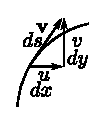
\includegraphics[scale=1.8]{figure/chapter3/3-1-2.eps}
%\caption{\label{fig:blue_rectangle} Rectangle}
\end{figure}
\end{minipage}\\
%----------------------
\item Stream tube and vorticity tube (3D expression)
\begin{figure}[H]
\centering
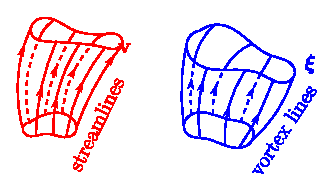
\includegraphics[scale=1.8]{figure/chapter3/3-1-3.eps}
%\caption{\label{fig:blue_rectangle} Rectangle}
\end{figure}
\item Circulation\\
Define circulation\\
%----------------------
\begin{minipage}{0.4\textwidth}
\begin{equation}
\Gamma = \oint_C\mathbf{v}\cdot\mathbf{t}dl
\label{eq: 3-1-3}
\end{equation}
\end{minipage} \hfill
\begin{minipage}{0.4\textwidth}
\begin{figure}[H]
\centering
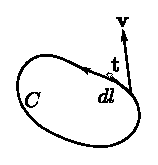
\includegraphics[scale=1.8]{figure/chapter3/3-1-4.eps}
%\caption{\label{fig:blue_rectangle} Rectangle}
\end{figure}
\end{minipage}\\
%----------------------
From Stokes' theorem
\begin{align*}
\Gamma = \oint_C\mathbf{v}\cdot\mathbf{t}dl 
&= \iint_S\mathbf{n}\cdot\left(\nabla\times\mathbf{v}\right) dS \\
&= \iint_S\mathbf{n}\cdot\boldsymbol{\xi}dS
\end{align*}
$\boldsymbol{\xi}=\mathbf{0}$ at all points enclosed in $C\Longrightarrow\Gamma = 0$ around $C$.\\
$\Gamma = 0$ for every loop in the flow field ($\Longrightarrow$circulation-free flow field) \\
$\vc{}{\Longrightarrow}{\xcancel{\Longleftarrow}}\footnotemark \Gamma = 0$ everywhere in the flow field ($\Longrightarrow$irrotational flow field)\footnotetext{can reverted only for simply-connected region}
\item Kinematic of vorticity lines\\
Since $\nabla\cdot\left(\nabla\times\mathbf{v}\right) = 0\Longrightarrow\boxed{\nabla\cdot\boldsymbol{\xi} = 0}$, there can be no source or sink of vorticity, i.e., vorticity line must either forms a closed loop or must terminate on the boundary. (Part of the Helmholtz Theorem). Furthermore, for a closed region $\volume$
\[
{\oiint \hspace{-23.5pt} \int}_{\volume}\nabla\cdot\boldsymbol{\xi}d\volume \vc{=}{\text{div.}}{\text{thm.}} \oiint_S\mathbf{n}\cdot\boldsymbol{\xi}dS = 0
\]
If the closed region is a section of a vorticity tube
%----------------------
\begin{minipage}{0.4\textwidth}
\begin{align*}
&\iint_{S_1}\mathbf{n}\cdot\boldsymbol{\xi}dS + \iint_{S_2}\mathbf{n}\cdot\boldsymbol{\xi}dS = 0 \\
\Longrightarrow
&-\oint_{C_1}\mathbf{v}\cdot\mathbf{t}dl + \oint_{C_2}\mathbf{v}\cdot\mathbf{t}dl = 0\\
\Longrightarrow
&\boxed{\Gamma_{C_1} = \Gamma_{C_2}}\phantom{-} (\abs{\xi_1}S_1=\abs{\xi_2}S_2)
\end{align*}
\end{minipage} \hfill
\begin{minipage}{0.4\textwidth}
\begin{figure}[H]
\centering
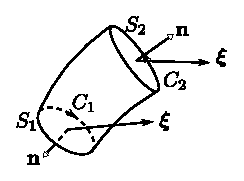
\includegraphics[scale=1.8]{figure/chapter3/3-1-5.eps}
%\caption{\label{fig:blue_rectangle} Rectangle}
\end{figure}
\end{minipage}\\
%----------------------
i.e., the circulation of each cross section of a vorticity tube is a \emph{constant} (Part of the Helmholtz Theorem).
\begin{figure}[H]
\centering
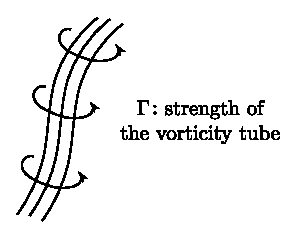
\includegraphics[scale=1.8]{figure/chapter3/3-1-6.eps}
%\caption{\label{fig:blue_rectangle} Rectangle}
\end{figure}
\end{itemize}
\subsection{Stream Function and Potential Function}
\begin{itemize}
\item Potential function\\
A vector field $\mathbf{v}(\mathbf{x},t)$ satisfying $\nabla\times\mathbf{v} = \mathbf{0}$ everywhere is called the \emph{irrotational field}. \\
If $\mathbf{v}$ is velocity field of a flow $\Longrightarrow$ \emph{irrotational field}. \\
Can represent $\mathbf{v}$ by the gradient of a scalar function $\Phi(\mathbf{x},t)$, i.e.
\begin{equation}
\mathbf{v} = \nabla\Phi\text{ (since $\nabla\times\left(\nabla\Phi\right) = \mathbf{0}$)}
\label{eq: 3-1-4}
\end{equation}
where $\Phi$ is scalar (velocity) potential function.
\item Steam function\\
A vector field $\mathbf{v}(\mathbf{x},t)$ satisfying $\nabla\cdot\mathbf{v} = 0$ everywhere is called the \emph{solenoidal field}. \\
If $\mathbf{v}$ is velocity field of a flow $\Longrightarrow$ \emph{solenoidal field}. \\
Can represent $\mathbf{v}$ by the curl of a scalar function $\boldsymbol{\Psi}(\mathbf{x},t)$, i.e.
\begin{equation}
\mathbf{v} = \nabla\times\boldsymbol{\Psi}\text{ (since $\nabla\cdot\left(\nabla\times\boldsymbol{\Psi}\right) = 0$)}
\label{eq: 3-1-5}
\end{equation}
where $\boldsymbol{\Psi}$ is vector potential function. (Note: $\Psi$ is not uniquely determinated by $\mathbf{v}$)
\end{itemize}
Specially for a 2D incompressible flow\\
Since $\mathbf{v} = u(x,y,t)\mathbf{e_x} + v(x,y,t)\mathbf{e_y}$ only, can show that \eqref{eq: 3-1-5} is satisfied with
\[
\boldsymbol{\Psi} = 0\mathbf{e_x} + 0\mathbf{e_y} + \psi(x,y,t)\mathbf{e_z}
\]
where $\psi$ is streamfunction for 2D incompressible flows.
\begin{exercise}
Show that $u\mathbf{e_x} + v\mathbf{e_y} = \nabla\times\boldsymbol{\Psi}$
\end{exercise}
and 
\begin{align*}
u = \frac{\partial\psi}{\partial y}, &&v = -\frac{\partial\psi}{\partial x}
\end{align*}
in polar coordinate, $\psi = \psi(r,\theta,t)$
\begin{align*}
v_r = \frac{1}{r}\frac{\partial\psi}{\partial\theta}, &&v_\theta = - \frac{\partial\psi}{\partial r}
\end{align*}
\begin{exercise}
Show that the vector potential for axisymmetric incompressible flow can be chosen as
\begin{enumerate}[label = \protect\circled{\arabic*}]
\item in cylindrical coordinate ($r,\theta,z$)
\begin{align*}
v_r = v_r(r,z,t), && v_z = v_z(r,z,t), && v_\theta = 0
\end{align*}
\begin{equation}
\boldsymbol{\Psi} = \psi_\theta\mathbf{e_\theta} = \underbrace{\frac{1}{r}\psi(r,z,t)}_{\psi_\theta}\mathbf{e_\theta}
\end{equation}
\[
\nabla\times\boldsymbol{\Psi} = \frac{1}{r}
\begin{vmatrix}
\mathbf{e_r} & r\mathbf{e_\theta} & \mathbf{e_z} \\
\displaystyle\frac{\partial}{\partial r} & \displaystyle\frac{\partial}{\partial\theta} & \displaystyle\frac{\partial}{\partial z} \\
0 & r\psi_\theta & 0
\end{vmatrix}
= v_r\mathbf{e_r} + v_z\mathbf{e_z}
\]
then $\mathbf{v} = \nabla\times\boldsymbol{\Psi}$ 
\begin{align*}
\Longrightarrow
v_r = -\frac{1}{r}\frac{\partial\psi}{\partial z}, && v_z = \frac{1}{r}\frac{\partial\psi}{\partial r}
\end{align*}
where $\psi$ is Stokes' stream function.
\item in spherical coordinate ($r,\theta,\phi$)
\begin{align*}
v_r = v_r(r,\theta,t), && v_\theta = v_\theta(r,\phi,t), && v_\phi = 0
\end{align*}
\begin{equation}
\boldsymbol{\Psi} = \psi_\phi\mathbf{e_\phi} = \underbrace{\frac{1}{r\sin\theta}\psi(r,\theta,t)}_{\psi_\theta}\mathbf{e_\phi}
\end{equation}
\[
\nabla\times\boldsymbol{\Psi} = \frac{1}{r^2\sin\theta}
\begin{vmatrix}
\mathbf{e_r} & r\mathbf{e_\theta} & r\sin\theta\mathbf{e_\phi} \\
\displaystyle\frac{\partial}{\partial r} & \displaystyle\frac{\partial}{\partial\theta} & \displaystyle\frac{\partial}{\partial \phi} \\
0 & 0 & r\sin\theta\psi_\phi\mathbf{e_\phi}
\end{vmatrix}
= v_r\mathbf{e_r} + v_\theta\mathbf{e_\theta}
\]
then $\mathbf{v} = \nabla\times\boldsymbol{\Psi}$ 
\begin{align*}
\Longrightarrow
v_r = \frac{1}{r^2\sin\theta}\frac{\partial\psi}{\partial \theta}, && v_\theta = -\frac{1}{r}\frac{\partial\psi}{\partial r}
\end{align*}
where $\psi$ is Stokes' stream function.
\begin{figure}[H]
\centering
\subfigure[cylindrical coordinate ($r,\theta,z$)]
{
%\label{3-7-Plot of frequency response in amplitude}
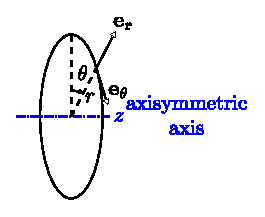
\includegraphics[scale=1.5]{figure/chapter3/3-1-8.eps}
}
\centering
\subfigure[spherical coordinate($r,\theta,\phi$)]
{
%\label{3-7-Plot of frequency response in phase}
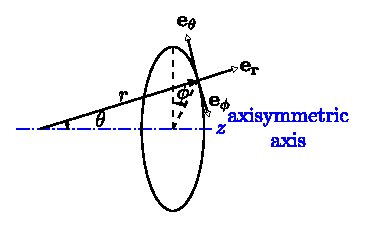
\includegraphics[scale=1.5]{figure/chapter3/3-1-7.eps}
}
%\caption{Plot of frequency response}
\end{figure}
\end{enumerate}
\end{exercise}

\section{Dynamics}
\subsection{Bernoulli equation}
(for inviscid fluid, $\mu = \lambda = 0,\boldsymbol{\tau} = - p\mathbf{I}$ only)\\
Euler equation 
\begin{equation}
\rho\frac{D\mathbf{v}}{Dt} = \rho\mathbf{g} - \nabla p
\label{eq: 3-2-1}
\end{equation}
Now
\[
\frac{D\mathbf{v}}{Dt} = \frac{\partial\mathbf{v}}{\partial t} + \mathbf{v}\cdot\nabla\mathbf{v} = \frac{\partial\mathbf{v}}{\partial t} + \nabla\left(\frac{v^2}{2}\right) - \mathbf{v}\times\boldsymbol{\xi}
\]
\begin{exercise}
Show that vector identity
\[
\mathbf{v}\times\left(\nabla\times\mathbf{v}\right) = \nabla\left(\frac{1}{2}\mathbf{v}\cdot\mathbf{v}\right)- \mathbf{v}\cdot\nabla\mathbf{v} 
\]
\end{exercise}
and $\nabla\times\mathbf{g} = \mathbf{0}$ (conservative force field)\\
$\Longrightarrow\mathbf{g} = -\nabla U$ ($U\colon$ gravitational force)\\
\begin{equation}
\eqref{eq: 3-2-1}\Longrightarrow
\frac{\partial\mathbf{v}}{\partial t} + \nabla\left(\frac{v^2}{2}\right) - \mathbf{v}\times\boldsymbol{\xi} = -\nabla U - \frac{\nabla p}{\rho}
\label{eq: 3-2-2}
\end{equation}
\begin{itemize}
\item  Steady flow along the streamline\\
Let $d\mathbf{s}\parallel$ a special streamline (i.e.$d\mathbf{s}\perp\mathbf{v}$ along streamline)
\[
\begin{aligned}
d\mathbf{s}\cdot\eqref{eq: 3-2-2}
\Longrightarrow &d\mathbf{s}\cdot\nabla\left(\frac{v^2}{2}\right) - \cancelto{0\because\left(\mathbf{v}\times\boldsymbol{\xi}\right)\perp d\mathbf{s}}{d\mathbf{s}\cdot\left(\mathbf{v}\times\mathbf{\xi}\right)}\\ 
&= -d\mathbf{s}\cdot\nabla U - d\mathbf{s}\cdot\frac{\nabla p}{\rho}\\
\Longrightarrow & d\left(\frac{v^2}{2}\right) + \frac{dp}{\rho} + dU = 0
\end{aligned}
\]
integrate (along streamline)
\begin{subequations}
\begin{align}
\Longrightarrow\int\frac{dp}{\rho} + \frac{v^2}{2} + U = \text{ constant (along streamline)}
\label{eq: 3-2-3}
\end{align}
For ideal fluid, $\rho = $ constant
\begin{align}
\eqref{eq: 3-2-3}\Longrightarrow
\frac{p}{\rho} + \frac{v^2}{2} + U = \text{ constant (along streamline)}
\label{eq: 3-2-4}
\end{align}
(Mechanical energy is conserved.)
\end{subequations}
\item Unsteady, \emph{irrotational}, and \emph{barotropic} flow\\
irrotational $\Longrightarrow\boldsymbol{\xi} = \mathbf{0}$ and $\mathbf{v} = \nabla\Phi$\\
barotropic $\Longrightarrow\rho = \rho(p)$ (or $p = p(\rho)$) 
\begin{exercise}
Show that 
\[
\Longrightarrow\frac{\nabla p}{\rho} = \nabla\int\frac{dp}{\rho}
\]
\end{exercise}
\eqref{eq: 3-2-1} reduces to
\[
\nabla\left\{\frac{\partial\Phi}{\partial t} + \frac{v^2}{2} + U + \int\frac{dp}{\rho} = 0\right\}
\]
\begin{equation}
\Longrightarrow\frac{\partial\Phi}{\partial t} + \int\frac{dp}{\rho} + \frac{1}{2}\nabla\Phi\cdot\nabla\Phi + U = f(t)
\label{eq: 3-2-5}
\end{equation}
For steady and incompressible
\[
\eqref{eq: 3-2-5}\Longrightarrow
\boxed{
\frac{p}{\rho} + \frac{1}{2}\nabla\Phi\cdot\nabla\Phi + U = \text{ constant }}
\]
(for ideal fluid + irrotation) everywhere
\end{itemize}
\subsection{Kelvin's Circulation Theorem}
Euler equation
\[
\frac{D\mathbf{v}}{Dt} = -\frac{\nabla p}{\rho} + \frac{\mathbf{f_b}}{\rho}
\]
where $\mathbf{f_b}$ is body force/mass
\begin{figure}[H]
\centering
%\subfigure[cylindrical coordinate ($r,\theta,z$)]
{
%\label{3-7-Plot of frequency response in amplitude}
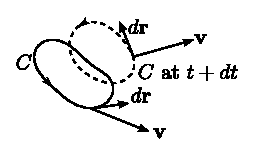
\includegraphics[scale=1.5]{figure/chapter3/3-2-1.eps}
}
\centering
%\subfigure[spherical coordinate($r,\theta,\phi$)]
{
%\label{3-7-Plot of frequency response in phase}
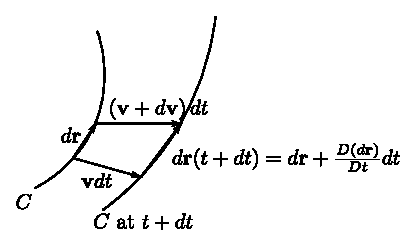
\includegraphics[scale=1.5]{figure/chapter3/3-2-2.eps}
}
%\caption{Plot of frequency response}
\end{figure}
\begin{align*}
&d\mathbf{r} + \left(\mathbf{v} + d\mathbf{v}\right)dt = \mathbf{v}dt + d\mathbf{r} + \frac{D\left(d\mathbf{r}\right)}{Dt}dt \\
\Longrightarrow
&\frac{D\left(d\mathbf{r}\right)}{Dt} = d\mathbf{v}
\end{align*}
or
\[
\frac{D\left(d\mathbf{r}\right)}{Dt} = d\frac{D\mathbf{r}}{Dt} = d\mathbf{v}
\]
Consider around a closed curve curve $C$
\begin{align*}
\Gamma &= \oint_C\mathbf{v}\cdot d\mathbf{r} \\
\frac{D\Gamma}{Dt} &= \frac{D}{Dt}\oint_C\mathbf{v}\cdot d\mathbf{r} \\
&= \oint_C\left[\frac{D\mathbf{v}}{Dt}\cdot d\mathbf{r} + \mathbf{v}\cdot\frac{D\left(d\mathbf{r}\right)}{Dt}\right] \\
&= \oint_C\left[\frac{D\mathbf{v}}{Dt}\cdot d\mathbf{r} + \mathbf{v}\cdot d\mathbf{v}\right]
\end{align*}
Now
\begin{enumerate}[label = \protect\circled{\arabic*}]
\item
\begin{align*}
\oint_C\frac{D\mathbf{v}}{Dt}\cdot d\mathbf{r}
&= \oint_C\left(-\frac{\nabla p}{\rho} + \frac{\mathbf{f_b}}{\rho}\right)\cdot d\mathbf{r} \\
&= \iint_S\mathbf{n}\cdot\mathbf{B} dS
\end{align*}
with
\[
\mathbf{B} = \nabla\times\left[-\frac{\nabla p}{\rho} + \frac{\mathbf{f_b}}{\rho}\right]
\]
\item
\[
\oint_C\mathbf{v}\cdot d\mathbf{v} = \oint_C d\left(\frac{v^2}{2}\right) = 0
\]
as long as no discontinuity in $v^2/2$ existing along the curve $C$
Hence
\begin{equation}
\boxed{\frac{D\Gamma}{Dt} = \iint_S\mathbf{n}\cdot\mathbf{B} dS} \text{ (Bjerknes Theorem)}
\label{eq: 3-2-6}
\end{equation}
i.e., rate of circulation is caused by the rotationality of either surface force $\nabla p /\rho$ or body force $\mathbf{f_b}/\rho$.\\
If the flow is barotropic (i.e. $\rho = \rho (p)$ or $p = p(\rho)$ only)
\[
\frac{\nabla p}{\rho} = \nabla\int\frac{dp}{\rho}
\]
and the body force is conservative, i.e., 
\[
\frac{\mathbf{f_b}}{\rho} = -\nabla U
\]
then
\[
\mathbf{B} = \nabla\times\left[-\nabla\int\frac{dp}{\rho} - \nabla U\right] = \mathbf{0}
\]
\begin{equation}
\boxed{
\frac{D\Gamma}{Dt} = 0
}\text{ (Kelvin's Theorem)}
\label{eq: 3-2-7}
\end{equation}
i.e., circulation around any closed material curve is \emph{conserved} in an \emph{inviscid}, \emph{barotropic} (or $\rho =$ constant), and \emph{conservative body force field}. 
%\input{test.tex}
\end{enumerate}

\begin{discussion}\mbox{}\\
\begin{enumerate}[label = \protect\circled{\arabic*}]
\item The flow does not have to be irrotational ($\boldsymbol{\xi}=\mathbf{0}$)
\item Kelvin's theorem implies that all motions started from rest (i.e., $\Gamma = 0$ for every loop initially) must be circulation free (i.e. irrotational) at any subsequent instant.
\item Eq .\eqref{eq: 3-2-7} also applies to

%
\begin{tikzpicture} 
\coordinate (C1) at (1.2,0);
\node[below right] at (C1){$C$};
\coordinate (C2) at (2.2,0);
\node[below right] at (C2){$C'$};
\coordinate (C3) at (3.2,0);
\node[below right] at (C3){$C''$};
\coordinate (C4) at (4.2,0);
\node[right] at (C4){$\displaystyle\frac{D\Gamma}{Dt} = 0$};
\draw[->] (-3,1) -- (-2,1);
\draw[->] (-3,0) -- (-2,0);
\draw[->] (-3,-1) -- (-2,-1);
\filldraw[color=blue!60, fill=blue!10](0,0) circle (1);
\draw[color=blue!60 ,pattern=hatch, pattern color=blue!60, hatch size=10pt, hatch angle=0](0,0) circle (1);

% \draw (2.5,0) ellipse (1.5 and 0.5);
\draw [-{Latex[length=2mm]}, rotate=0] (C1) arc [start angle=-360, end angle=0, x radius=1.2cm, y radius=1.2cm];
\draw [-{Latex[length=2mm]}, rotate=0] (C2) arc [start angle=-360, end angle=0, x radius=1.8cm, y radius=1.4cm];
\draw [-{Latex[length=2mm]}, rotate=0] (C3) arc [start angle=-360, end angle=0, x radius=2.4cm, y radius=1.6cm];
\end{tikzpicture}

\vspace{5em}

\begin{tikzpicture}[scale=6,transform canvas]
\newcommand{\la}{0.5}
\newcommand{\lb}{-0.1}
\begin{scope}[rotate=-5]
	\filldraw[color=blue!60, fill=blue!10, line width=0.04mm] 
(1.0000000,0.0005993) -- 
(0.9900000,0.0029690) --
(0.9800000,0.0053335) -- 
(0.9700000,0.0076868) -- 
(0.9600000,0.0100232) -- 
(0.9400000,0.0146239) -- 
(0.9200000,0.0191156) -- 
(0.9000000,0.0235025) -- 
(0.8800000,0.0277891) -- 
(0.8600000,0.0319740) -- 
(0.8400000,0.0360536) -- 
(0.8200000,0.0400245) -- 
(0.8000000,0.0438836) -- 
(0.7800000,0.0476281) -- 
(0.7600000,0.0512565) -- 
(0.7400000,0.0547675) -- 
(0.7200000,0.0581599) -- 
(0.7000000,0.0614329) -- 
(0.6800000,0.0645843) -- 
(0.6600000,0.0676046) -- 
(0.6400000,0.0704822) -- 
(0.6200000,0.0732055) -- 
(0.6000000,0.0757633) -- 
(0.5800000,0.0781451) -- 
(0.5600000,0.0803480) -- 
(0.5400000,0.0823712) -- 
(0.5200000,0.0842145) -- 
(0.5000000,0.0858772) -- 
(0.4800000,0.0873572) -- 
(0.4600000,0.0886427) -- 
(0.4400000,0.0897175) -- 
(0.4200000,0.0905657) -- 
(0.4000000,0.0911712) -- 
(0.3800000,0.0915212) -- 
(0.3600000,0.0916266) -- 
(0.3400000,0.0915079) -- 
(0.3200000,0.0911857) -- 
(0.3000000,0.0906804) -- 
(0.2800000,0.0900016) -- 
(0.2600000,0.0890840) -- 
(0.2400000,0.0878308) -- 
(0.2200000,0.0861433) -- 
(0.2000000,0.0839202) -- 
(0.1800000,0.0810687) -- 
(0.1600000,0.0775707) -- 
(0.1400000,0.0734360) -- 
(0.1200000,0.0686204) -- 
(0.1000000,0.0629981) -- 
(0.0800000,0.0564308) -- 
(0.0600000,0.0487571) -- 
(0.0500000,0.0442753) -- 
(0.0400000,0.0391283) -- 
(0.0300000,0.0330215) -- 
(0.0200000,0.0253735) -- 
(0.0120000,0.0178581) -- 
(0.0080000,0.0137350) -- 
(0.0040000,0.0089238) -- 
(0.0020000,0.0058025) -- 
(0.0010000,0.0037271) -- 
(0.0005000,0.0023390) -- 
(0.0000000,0.0000000) coordinate (y) -- 
(0.0005000,-.0046700) -- 
(0.0010000,-.0059418) -- 
(0.0020000,-.0078113) -- 
(0.0040000,-.0105126) -- 
(0.0080000,-.0142862) -- 
(0.0120000,-.0169733) -- 
(0.0200000,-.0202723) -- 
(0.0300000,-.0226056) -- 
(0.0400000,-.0245211) -- 
(0.0500000,-.0260452) -- 
(0.0600000,-.0271277) -- 
(0.0800000,-.0284595) -- 
(0.1000000,-.0293786) -- 
(0.1200000,-.0299633) -- 
(0.1400000,-.0302404) -- 
(0.1600000,-.0302546) -- 
(0.1800000,-.0300490) -- 
(0.2000000,-.0296656) -- 
(0.2200000,-.0291445) -- 
(0.2400000,-.0285181) -- 
(0.2600000,-.0278164) -- 
(0.2800000,-.0270696) -- 
(0.3000000,-.0263079) -- 
(0.3200000,-.0255565) -- 
(0.3400000,-.0248176) -- 
(0.3600000,-.0240870) -- 
(0.3800000,-.0233606) -- 
(0.4000000,-.0226341) -- 
(0.4200000,-.0219042) -- 
(0.4400000,-.0211708) -- 
(0.4600000,-.0204353) -- 
(0.4800000,-.0196986) -- 
(0.5000000,-.0189619) -- 
(0.5200000,-.0182262) -- 
(0.5400000,-.0174914) -- 
(0.5600000,-.0167572) -- 
(0.5800000,-.0160232) -- 
(0.6000000,-.0152893) -- 
(0.6200000,-.0145551) -- 
(0.6400000,-.0138207) -- 
(0.6600000,-.0130862) -- 
(0.6800000,-.0123515) -- 
(0.7000000,-.0116169) -- 
(0.7200000,-.0108823) -- 
(0.7400000,-.0101478) -- 
(0.7600000,-.0094133) -- 
(0.7800000,-.0086788) -- 
(0.8000000,-.0079443) -- 
(0.8200000,-.0072098) -- 
(0.8400000,-.0064753) -- 
(0.8600000,-.0057408) -- 
(0.8800000,-.0050063) -- 
(0.9000000,-.0042718) -- 
(0.9200000,-.0035373) -- 
(0.9400000,-.0028028) -- 
(0.9600000,-.0020683) -- 
(0.9700000,-.0017011) -- 
(0.9800000,-.0013339) -- 
(0.9900000,-.0009666) -- 
(1.0000000,-.0005993) coordinate (x);
%
\draw[color=blue!60 ,pattern=hatch, pattern color=blue!60, hatch size=10pt, hatch angle=0]
(1.0000000,0.0005993) -- 
(0.9900000,0.0029690) -- 
(0.9800000,0.0053335) -- 
(0.9700000,0.0076868) -- 
(0.9600000,0.0100232) -- 
(0.9400000,0.0146239) -- 
(0.9200000,0.0191156) -- 
(0.9000000,0.0235025) -- 
(0.8800000,0.0277891) -- 
(0.8600000,0.0319740) -- 
(0.8400000,0.0360536) -- 
(0.8200000,0.0400245) -- 
(0.8000000,0.0438836) -- 
(0.7800000,0.0476281) -- 
(0.7600000,0.0512565) -- 
(0.7400000,0.0547675) -- 
(0.7200000,0.0581599) -- 
(0.7000000,0.0614329) -- 
(0.6800000,0.0645843) -- 
(0.6600000,0.0676046) -- 
(0.6400000,0.0704822) -- 
(0.6200000,0.0732055) -- 
(0.6000000,0.0757633) -- 
(0.5800000,0.0781451) -- 
(0.5600000,0.0803480) -- 
(0.5400000,0.0823712) -- 
(0.5200000,0.0842145) -- 
(0.5000000,0.0858772) -- 
(0.4800000,0.0873572) -- 
(0.4600000,0.0886427) -- 
(0.4400000,0.0897175) -- 
(0.4200000,0.0905657) -- 
(0.4000000,0.0911712) -- 
(0.3800000,0.0915212) -- 
(0.3600000,0.0916266) -- 
(0.3400000,0.0915079) -- 
(0.3200000,0.0911857) -- 
(0.3000000,0.0906804) -- 
(0.2800000,0.0900016) -- 
(0.2600000,0.0890840) -- 
(0.2400000,0.0878308) -- 
(0.2200000,0.0861433) -- 
(0.2000000,0.0839202) -- 
(0.1800000,0.0810687) -- 
(0.1600000,0.0775707) -- 
(0.1400000,0.0734360) -- 
(0.1200000,0.0686204) -- 
(0.1000000,0.0629981) -- 
(0.0800000,0.0564308) -- 
(0.0600000,0.0487571) -- 
(0.0500000,0.0442753) -- 
(0.0400000,0.0391283) -- 
(0.0300000,0.0330215) -- 
(0.0200000,0.0253735) -- 
(0.0120000,0.0178581) -- 
(0.0080000,0.0137350) -- 
(0.0040000,0.0089238) -- 
(0.0020000,0.0058025) -- 
(0.0010000,0.0037271) -- 
(0.0005000,0.0023390) -- 
(0.0000000,0.0000000) -- 
(0.0005000,-.0046700) -- 
(0.0010000,-.0059418) -- 
(0.0020000,-.0078113) -- 
(0.0040000,-.0105126) -- 
(0.0080000,-.0142862) -- 
(0.0120000,-.0169733) -- 
(0.0200000,-.0202723) -- 
(0.0300000,-.0226056) -- 
(0.0400000,-.0245211) -- 
(0.0500000,-.0260452) -- 
(0.0600000,-.0271277) -- 
(0.0800000,-.0284595) -- 
(0.1000000,-.0293786) -- 
(0.1200000,-.0299633) -- 
(0.1400000,-.0302404) -- 
(0.1600000,-.0302546) -- 
(0.1800000,-.0300490) -- 
(0.2000000,-.0296656) -- 
(0.2200000,-.0291445) -- 
(0.2400000,-.0285181) -- 
(0.2600000,-.0278164) -- 
(0.2800000,-.0270696) -- 
(0.3000000,-.0263079) -- 
(0.3200000,-.0255565) -- 
(0.3400000,-.0248176) -- 
(0.3600000,-.0240870) -- 
(0.3800000,-.0233606) -- 
(0.4000000,-.0226341) -- 
(0.4200000,-.0219042) -- 
(0.4400000,-.0211708) -- 
(0.4600000,-.0204353) -- 
(0.4800000,-.0196986) -- 
(0.5000000,-.0189619) -- 
(0.5200000,-.0182262) -- 
(0.5400000,-.0174914) -- 
(0.5600000,-.0167572) -- 
(0.5800000,-.0160232) -- 
(0.6000000,-.0152893) -- 
(0.6200000,-.0145551) -- 
(0.6400000,-.0138207) -- 
(0.6600000,-.0130862) -- 
(0.6800000,-.0123515) -- 
(0.7000000,-.0116169) -- 
(0.7200000,-.0108823) -- 
(0.7400000,-.0101478) -- 
(0.7600000,-.0094133) -- 
(0.7800000,-.0086788) -- 
(0.8000000,-.0079443) -- 
(0.8200000,-.0072098) -- 
(0.8400000,-.0064753) -- 
(0.8600000,-.0057408) -- 
(0.8800000,-.0050063) -- 
(0.9000000,-.0042718) -- 
(0.9200000,-.0035373) -- 
(0.9400000,-.0028028) -- 
(0.9600000,-.0020683) -- 
(0.9700000,-.0017011) -- 
(0.9800000,-.0013339) -- 
(0.9900000,-.0009666) -- 
(1.0000000,-.0005993);;
\end{scope}
\coordinate (z) at (y |- x);
\coordinate (vtip) at ($(x) + (\la,\lb)$);
\node[below] at ($(vtip) + (0.02,0)$){vortex sheet};

\draw[-] (x.east) .. controls +(down:0mm) and +(left:1mm) .. (vtip.west);
\coordinate (vtip middle) at ($(x)!0.25!(vtip)$);
\coordinate (vtip middle top) at ($(vtip middle) + (0,0.2)$);
\coordinate (vtip middle bottom) at ($(vtip middle) + (0,-0.2)$);
\draw[-] (vtip middle) -- (vtip middle top);
\draw[-] (vtip middle) -- (vtip middle bottom); 

\foreach \v in {0.2,0.4,0.6,0.8}{
	\draw[->]  ($(vtip middle)!\v!(vtip middle top)$) -- ($(vtip middle)!\v!(vtip middle top) + (0.2,0)$);    
    }
%
\foreach \v in {0.2,0.4,0.6,0.8}{
	\draw[->]  ($(vtip middle)!\v!(vtip middle bottom)$) -- ($(vtip middle)!\v!(vtip middle bottom) + (0.1,0)$);    
    }
\draw [-{Latex[length=2mm]}, rotate=0] ($(vtip) + (-0.48, 0.5)$) arc [start angle=-300, end angle=60, x radius=0.7cm, y radius=0.45cm];
\node[above right] at ($(vtip) + (-0.5, 0.5)$){$\displaystyle C'\rightarrow\frac{D\Gamma}{Dt}\neq 0$};
\draw [-{Latex[length=2mm]}, rotate=0] ($(vtip) + (0.24,-0.05)$) arc [start angle=-380, end angle=-20, x radius=1.0cm, y radius=0.6cm];
\node[below right] at ($(vtip) + (0.2,-0.05)$){$\displaystyle C\rightarrow\frac{D\Gamma}{Dt}= 0$};
\end{tikzpicture}

\vspace{5em}

\item \mbox{}\\ 
\begin{enumerate}[label = (\alph*)]
\item \label{ch3-2-dis-a} Helmholtz theorem: $\Gamma =$constant around the cross-section of a vorticity tube
\item \label{ch3-2-dis-b} Kelvin's theorem: $\Gamma =$constant around a material closed curve 
\item \label{ch3-2-dis-c} Can show that Kelvin's theorem $\Longrightarrow$ vorticity line is a material 
\end{enumerate}
i.e., once a vorticity line (tube), always a vorticity line (tube).\\
Hence \ref{ch3-2-dis-a} + \ref{ch3-2-dis-b} + \ref{ch3-2-dis-c} $\Longrightarrow$ circulation $\Gamma$ around a vorticity tube is preserved along its motion (in an inviscid, barotropic, and conservative-body force field)
\begin{figure}[H]
\centering
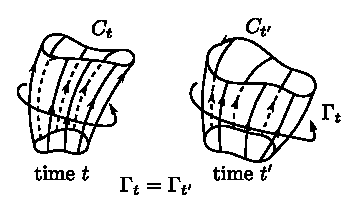
\includegraphics[scale=1.8]{figure/chapter3/3-2-5.eps}
%\caption{\label{fig:blue_rectangle} Rectangle}
\end{figure}
\item Summary of the Helmholtz Vortex Theorem
\begin{enumerate}[label = (\alph*)]
\item $\nabla\cdot\boldsymbol{\xi} = 0\Longrightarrow$ Vorticity line either forms a closed loop or terminate at boundary
\item \label{ch3-2-dis-4-b}
\[
\iint_{S_1}\mathbf{n}\cdot\boldsymbol{\xi}dS = -\iint_{S_2}\mathbf{n}\cdot\boldsymbol{\xi}dS\Longrightarrow\Gamma_{C_1}=\Gamma_{C_2}
\]
\begin{figure}[H]
\centering
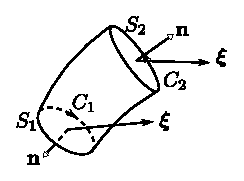
\includegraphics[scale=1.8]{figure/chapter3/3-2-6.eps}
%\caption{\label{fig:blue_rectangle} Rectangle}
\end{figure}
\item \label{ch3-2-dis-4-c} Vorticity line is a material line (in an inviscid, barotropic, and conservative-body force field)
\item \label{ch3-2-dis-4-d} $\displaystyle\frac{D\Gamma}{Dt}=0$ along any material closed curve, e.g. vortex ring\\
\begin{tikzpicture}
\begin{scope}[rotate=-30]
    \draw [-{Latex[length=2mm]}, rotate=0] ($(0, 0) + (2, 1.2)$) arc [start angle=60, end angle=220, x radius=0.9cm, y radius=0.8cm];
    \draw [-{Latex[length=2mm]}, rotate=0] ($(0, 0) + (-2, 1.2)$) arc [start angle=120, end angle=-40, x radius=0.9cm, y radius=0.8cm];
    \draw [-{Latex[length=2mm]}, rotate=0] ($(0, 0) + (-0.2, -1.7)$) arc [start angle=270, end angle=450, x radius=0.9cm, y radius=0.8cm];
    \draw (0,0) ellipse (3 and 1.5);
    \clip (0,-1.8) ellipse (3 and 2.5);
    \draw (0,2.2) ellipse (3 and 2.5);
    \clip (0,2.2) ellipse (3 and 2.5);
    \draw (0,-2.2) ellipse (3 and 2.5);
\end{scope}
\end{tikzpicture}
\item From \ref{ch3-2-dis-4-b} + \ref{ch3-2-dis-4-c} + \ref{ch3-2-dis-4-d} $\Longrightarrow$ circulation around a vorticity tube is preserved along its motion (in an inviscid, barotropic, and conservative-body force field)
\end{enumerate}
\end{enumerate}
\end{discussion}
\subsection{Vorticity Equation}
Euler Equation
\[
\frac{\partial\mathbf{v}}{\partial t} + \mathbf{v}\cdot\nabla\mathbf{v} = \frac{1}{\rho}\mathbf{g} - \frac{\nabla p}{\rho}
\]
\begin{equation}
\Longrightarrow
\frac{\partial\mathbf{v}}{\partial t} + \nabla\left(\frac{v^2}{2}\right) - \mathbf{v}\times\boldsymbol{\xi} = -\nabla U - \frac{\nabla p}{\rho}
\tag{$\ast$}
\label{eq: ch3-2-3-*}
\end{equation}
\begin{equation}
\nabla\times\eqref{eq: ch3-2-3-*}\Longrightarrow\frac{\partial\boldsymbol{\xi}}{\partial t} + 0 - \nabla\times\left(\mathbf{v}\times\boldsymbol{\xi}\right) = 0 - \nabla\times\left(\frac{\nabla p}{\rho}\right)
\tag{$\ast\ast$}
\label{eq: ch3-2-3-**}
\end{equation}
From vector identity
\[
\nabla\times\left(\mathbf{v}\times\boldsymbol{\xi}\right) = \mathbf{v}\cancelto{0}{\left(\nabla\cdot\boldsymbol{\xi}\right)} - \underbrace{\boldsymbol{\xi}\left(\nabla\cdot\mathbf{v}\right)}_{\nabla\cdot\mathbf{v}=-\frac{1}{\rho}\frac{D\rho}{Dt}} + \left(\boldsymbol{\xi}\cdot\nabla\right)\mathbf{v} - \left(\mathbf{v}\cdot\nabla\right)\boldsymbol{\xi}
\]
also
\begin{exercise}
\begin{align*}
\nabla\times\left(\frac{\nabla p}{\rho}\right) 
&= \frac{1}{\rho}\cancelto{0}{\nabla\times\nabla p} + \left(\nabla\frac{1}{\rho}\right)\times\nabla p \\
&= -\frac{1}{\rho^2}\nabla \rho\times\nabla p
\end{align*}
\end{exercise}
\begin{exercise}
\begin{equation}
\eqref{eq: ch3-2-3-**}\Longrightarrow
\frac{D}{Dt}\left(\frac{\boldsymbol{\xi}}{\rho}\right) = \frac{\boldsymbol{\xi}}{\rho}\cdot\nabla\mathbf{v} + \frac{1}{\rho^2}\nabla\rho\times\nabla p
\label{eq: 3-2-8}
\end{equation}
\end{exercise}
For barotropic flow ($\rho=\rho (p)$ or $p=p(\rho)$)
\[
p = p(\rho)\Longrightarrow\nabla p = \frac{dp}{d\rho}\nabla\rho\Longrightarrow\nabla p\parallel\nabla\rho\Longrightarrow\nabla\rho\times\nabla p = 0
\]
\begin{equation}
\eqref{eq: 3-2-8}\Longrightarrow\frac{D}{Dt}\left(\frac{\boldsymbol{\xi}}{\rho}\right) = \frac{\boldsymbol{\xi}}{\rho}\cdot\nabla\mathbf{v}
\label{eq: 3-2-9}
\end{equation}
(in an inviscid, barotropic, and conservative-body force field)\\
For ideal fluid ($\rho=$constant)
\begin{equation}
\eqref{eq: 3-2-8}\Longrightarrow
\boxed{
\frac{D\boldsymbol{\xi}}{Dt} = \boldsymbol{\xi}\cdot\nabla\mathbf{v}
}
\label{eq: 3-2-10}
\end{equation}
\begin{itemize}
\item In an inviscid, barotropic (or $\rho=$ constant) and conservative body-force field, a vorticity line is a material line.
\begin{equation}
\Longrightarrow
\frac{D\left(d\mathbf{r}\right)}{Dt} = d\mathbf{v} = d\mathbf{r}\cdot\nabla\mathbf{v}
\label{eq: 3-2-11}
\end{equation}
\begin{figure}[H]
\centering
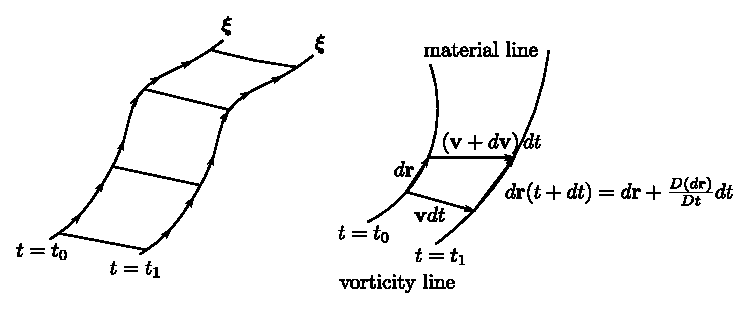
\includegraphics[scale=1.5]{figure/chapter3/3-2-7.eps}
%\caption{\label{fig:blue_rectangle} Rectangle}
\end{figure}
Now let $d\mathbf{r}$ be a segment of a vorticity line at $t=t_0$, i.e.
\[
\boldsymbol{\xi}\times d\mathbf{r} = \mathbf{0}\text{ (or $\boldsymbol{\xi}=\lambda d\mathbf{r}$) at } t=t_0
\]
\begin{align*}
\left[\frac{D\left(\boldsymbol{\xi}\times d\mathbf{r}\right)}{Dt}\right]_{t_0}
&= \left(\frac{D\boldsymbol{\xi}}{Dt}\times d\mathbf{r}\right)_{t_0} + \left(\boldsymbol{\xi}\times\frac{D\left(d\mathbf{r}\right)}{Dt}\right)_{t_0} \\
&= \left[\left(\boldsymbol{\xi}\cdot\nabla\mathbf{v}\right)\times d\mathbf{r}\right]_{t_0} + \left[\boldsymbol{\xi}\times d\mathbf{v}\right]_{t_0} \\
&= \left[\left(\lambda d\mathbf{r}\cdot\nabla\mathbf{v}\right)\times d\mathbf{r}\right]_{t_0} + \left[\lambda d\mathbf{r}\times d\mathbf{v}\right]_{t_0} \\
&= \left[\left(\lambda d\mathbf{v}\right)\times d\mathbf{r}\right]_{t_0} + \left[\lambda d\mathbf{r}\times d\mathbf{v}\right]_{t_0} = \mathbf{0}
\end{align*}
\[
\Longrightarrow \left(\boldsymbol{\xi}\times d\mathbf{r}\right)_{t+dt} = \left(\boldsymbol{\xi}\times d\mathbf{r}\right)_{t_0}
\]
\item The term $\boldsymbol{\xi}\cdot\nabla\mathbf{v}$ in vorticity equation
%----------------------
\begin{minipage}{0.4\textwidth}
Let $\boldsymbol{\xi}=\lambda d\mathbf{r}$\\
$\displaystyle\lambda(\mathbf{x},t) = \frac{\abs{\boldsymbol{\xi}}}{\abs{d\mathbf{r}}}$ vorticity/unit length\\
$\lambda\colon$ vorticity density
\end{minipage} \hfill
\begin{minipage}{0.4\textwidth}
\begin{figure}[H]
\centering
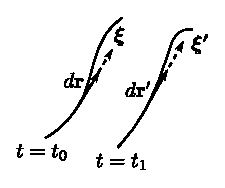
\includegraphics[scale=1.8]{figure/chapter3/3-2-8.eps}
%\caption{\label{fig:blue_rectangle} Rectangle}
\end{figure}
\end{minipage}\\
%----------------------
then 
\[
\frac{D\boldsymbol{\xi}}{Dt} = \boldsymbol{\xi}\cdot\nabla\mathbf{v}\Longrightarrow\frac{D\left(\lambda d\mathbf{r}\right)}{Dt} = \lambda d\mathbf{r}\cdot\nabla\mathbf{v}
\]
\[
\Longrightarrow\frac{D\lambda}{Dt}d\mathbf{r} + \lambda\underbrace{\frac{D\left(d\mathbf{r}\right)}{Dt}}_{d\mathbf{v}=d\mathbf{r}\cdot\nabla\mathbf{v}} = \lambda d\mathbf{r}\cdot\nabla\mathbf{v}
\]
\[
\Longrightarrow\boxed{\frac{D\lambda}{Dt} = 0}
\]
i.e., $\lambda$ is conserved when following fluid motion
\begin{figure}[H]
\centering
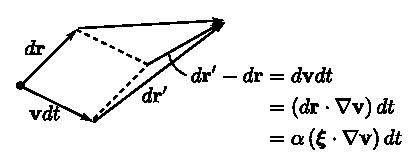
\includegraphics[scale=1.8]{figure/chapter3/3-2-9.eps}
%\caption{\label{fig:blue_rectangle} Rectangle}
\end{figure}
i.e., \emph{stretching} and \emph{turning} of the vorticity line in $dt$ is caused by the \emph{deformation rate field $\nabla\mathbf{v}$}.
\end{itemize}
\begin{note}\mbox{}\\
\begin{enumerate}[label = \protect\circled{\arabic*}]
\item The term $\boldsymbol{\xi}\cdot\nabla\mathbf{v}$ has important consequence in turbulent flow 
\begin{figure}[H]
\centering
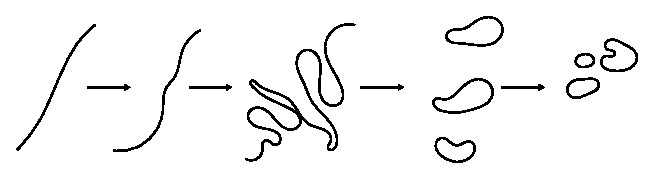
\includegraphics[scale=1.5]{figure/chapter3/3-2-10.eps}
%\caption{\label{fig:blue_rectangle} Rectangle}
\end{figure}
\item vorticity stretching effect
\begin{figure}[H]
\centering
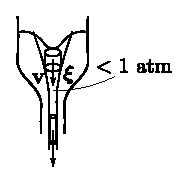
\includegraphics[scale=1.8]{figure/chapter3/3-2-11.eps}
%\caption{\label{fig:blue_rectangle} Rectangle}
\end{figure}
\end{enumerate}
\end{note}

\chapter{General Properties of Irrotational Motion in an Ideal Fluid (Potential Flows)}
\section{Basic Formulations of Potential Flows}
\subsection{Governing Equations}
Starting from irrotation: $\nabla\times\mathbf{v} = \mathbf{0}\Longrightarrow\mathbf{v} = \nabla\Phi$\\
For an ideal fluid, $\rho=$ constant, continuity equation: $\nabla\cdot\mathbf{v}=0$
\begin{equation}
\Longrightarrow\nabla\cdot\nabla\Phi = 0\Longrightarrow\boxed{\nabla^2\Phi = 0}\text{ (Laplace equation)}
\label{eq: 4-1-1}
\end{equation}
From Kelvin's circulation theorem
\[
\frac{D\Gamma}{Dt} =  0\text{ where }\Gamma = \oint_C\mathbf{v}\cdot\mathbf{t}dl
\]
hence if a flow field is circulation free flow (i.e. irrotational flow) initially, it will remain circulation free (i.e. irrotational) thereafter. The dynamics (i.e. pressure) of the flow field can be obtained from Bernoulli's equation, i.e.,
\begin{subequations}
\begin{align}
\frac{\partial\Phi}{\partial t} + \frac{p}{\rho} + \frac{1}{2}\nabla\Phi\cdot\nabla\Phi + U = f(t)
\label{eq: 4-1-2-a}
\end{align}
or redefine $\displaystyle\Phi \equiv\Phi-\int f(t)dt$
\begin{align}
\frac{\partial\Phi}{\partial t} + \frac{p}{\rho} + \frac{1}{2}\nabla\Phi\cdot\nabla\Phi + U = 0
\label{eq: 4-1-2-b}
\end{align}
\end{subequations}
Alternatively, staring from incompressibility: $\nabla\cdot\mathbf{v} = 0\Longrightarrow\mathbf{v} = \nabla\times\boldsymbol{\Psi}$\\
Use irrotaionality: $\nabla\times\mathbf{v} = \mathbf{0}$
\[
\Longrightarrow\nabla\times\left(\nabla\times\boldsymbol{\Psi}\right) = \mathbf{0}\Longrightarrow -\nabla^2\boldsymbol{\Psi} + \nabla\left(\nabla\cdot\boldsymbol{\Psi}\right) = \mathbf{0}
\]
\begin{note}
\[
\tilde{\boldsymbol{\Psi}} = \boldsymbol{\Psi} + \nabla A\Longrightarrow\nabla\times\tilde{\boldsymbol{\Psi}} = \nabla\times \boldsymbol{\Psi} + \cancelto{0}{\nabla\times\nabla A} = \mathbf{v}
\]
$\Longrightarrow\nabla\cdot\tilde{\boldsymbol{\Psi}} = \nabla\cdot\boldsymbol{\Psi} + \nabla^2A=0$, choose $A$ such that $\nabla^2A = -\nabla\cdot\boldsymbol{\Psi}$
\end{note}
Hence\footnote{Note that $\Psi$ is not uniquely determinated by $\mathbf{v}$}
\begin{equation}
\nabla^2\boldsymbol{\Psi} = 0
\label{eq: 4-1-3}
\end{equation}
\begin{enumerate}[label = (\alph*)]
\item For 2D flows\\
$\boldsymbol{\Psi} = \mathbf{e_z}\psi(x,y,t)$ only
\[
\Longrightarrow\nabla\cdot\boldsymbol{\Psi} = \frac{\partial\psi(x,y,t)}{\partial z} = 0
\]
therefore, governing equation: $\nabla\boldsymbol{\Psi} = 0\Longrightarrow\nabla^2\psi\mathbf{e_z} = \mathbf{0}$
\begin{equation}
\Longrightarrow\boxed{\nabla^2\psi = 0}
\end{equation}
(i.e. $\displaystyle\frac{\partial^2\psi}{\partial x^2} + \frac{\partial^2\psi}{\partial y^2} = 0$) (for 2D potential flow only))
\begin{exercise}{Show that for axisymmetric flows}\\
$\boldsymbol{\Psi}$ reduces to a vector of one component only and again $\nabla\cdot\boldsymbol{\Psi} = 0$, i.e.
\[
\boxed{\nabla^2\boldsymbol{\Psi} = 0}
\]
\begin{itemize}
\item for cylindrical coordinate ($r,z$)
\[
\nabla^2\left[\mathbf{e_\theta}\frac{1}{r}\psi(r,z,t)\right] = \mathbf{0}
\]
expanding:
\begin{equation}
\Longrightarrow\frac{\partial}{\partial r}\left(\frac{1}{r}\frac{\partial\psi}{\partial r}\right) + \frac{1}{r}\frac{\partial^2\psi}{\partial z^2} = 0
\label{eq: 4-1-4}
\end{equation}
(not a Laplace equation)
\item in spherical coordinate ($r,\theta$)
\[
\nabla^2\left[\mathbf{e_\varphi}\frac{1}{r\sin\theta}\psi(r,\theta,t)\right] = \mathbf{0}
\]
expanding:
\begin{equation}
\Longrightarrow\frac{\partial^2\psi}{\partial r^2} + \frac{\sin\theta}{r^2}\frac{\partial}{\partial\theta}\left(\frac{1}{\sin\theta}\frac{\partial\psi}{\partial\theta}\right) = 0
\label{eq: 4-1-4}
\end{equation}
\end{itemize}
\end{exercise}
\end{enumerate}
\subsection{Far-Field Boundary Conditions}
Consider the flow field generated by a solid body moving in an otherwise \emph{quiescent fluid}
\begin{tikzpicture}
    \filldraw[color=blue!60, fill=blue!10, tangent=0.1](0, 0) ellipse (1cm and 0.5cm);
    \draw[color=blue!60, pattern=hatch, pattern color=blue!60, hatch size=10pt, hatch angle=0](0,0) ellipse (1cm and 0.5cm);
    \draw [blue, ultra thick, use tangent, -latex] (0,0) -- (0,0.7) node [pos=0.7, anchor=east] {$\mathbf{n_S}$};
    \draw[color=blue!60, tangent=0.4](0, 0) ellipse (5cm and 4cm);
    \draw [blue, ultra thick, use tangent, -latex] (0,0) -- (0,-2) node [pos=1.0, anchor=east] {$\mathbf{n_{\Sigma}}$};
    \node[color=blue!60, above left] at ($(3,-3)$){$R$};
    \draw [color=blue!60, -{Latex[length=2mm]}, rotate=0] ($(4,0)$) arc [start angle=-190, end angle=-350, x radius=1.0cm, y radius=0.6cm] node [below] {$\Sigma$};
    \draw [color=blue!60, -{Latex[length=2mm]}, rotate=0] ($(0,0.2)$) arc [start angle=10, end angle=170, x radius=1.0cm, y radius=0.6cm] node [below] {$S$};
\end{tikzpicture}
\paragraph*{Neumann Extension Problem}\mbox{}\\
From divergence theorem
\[
\iiint_R\nabla^2\Phi d\volume = \oiint_S\mathbf{n_S}\cdot\nabla\Phi dS + \oiint_\Sigma\mathbf{n_{\Sigma}}\cdot\nabla\Phi d\Sigma
\]
\begin{align*}
\Longrightarrow
\oiint_\Sigma\mathbf{n_\Sigma}\cdot\nabla\Phi d\Sigma
&= -\oiint_S\underbrace{\mathbf{n_S}\cdot\nabla\Phi}_{=\mathbf{n}_S\cdot\mathbf{v_S\footnotemark}} dS \\
&= -\oiint_S\mathbf{n_S}\cdot\mathbf{v_S}dS = -\mathbf{v_S}\cdot\iint_S\mathbf{n_S}dS
\end{align*}
\footnotetext{no penetration on $S$}
i.e., 
\[
\oiint_\Sigma\mathbf{n_\Sigma}\cdot\nabla\Phi d\Sigma = 0
\]
Choose $\Sigma$ to be a large sphere with radius $r\to\infty$, then 
\[
\oiint_\Sigma\underbrace{\overbrace{\mathbf{n_Z}}^{=\mathbf{e}_r}\cdot\nabla\Phi}_{\displaystyle = \frac{\partial\Phi}{\partial r} = v_r}\overbrace{d\Sigma}^{=r^2\sin\theta d\theta d\varphi} = 0\Longrightarrow \oiint_\Sigma\underbrace{\frac{\partial\Phi}{\partial r}}_{=v_r}r^2\sin\theta d\theta d\varphi = 0
\]
\begin{equation}
\Longrightarrow v_r\equiv \frac{\partial\Phi}{\partial r}\sim o\left(\frac{1}{r^2}\right)
\end{equation}
Similarly, from divergence theorem\footnote{$\displaystyle\int_{\partial\mathcal{R}}\left(\cdot\right)n_idA = \int_\mathcal{R}\left(\cdot\right)_{,i}d\volume$}
\[
\iiint_R\cancelto{0}{\nabla\times\nabla\Phi}d\volume = \oiint_S\mathbf{n_S}\times\nabla\Phi dS + \oiint_\Sigma\mathbf{n_\Sigma}\times\nabla\Phi d\Sigma = 0
\]
\begin{align*}
\Longrightarrow
\oiint_\Sigma\mathbf{n_\Sigma}\times\nabla\Phi d\Sigma 
&= -\oiint_S\mathbf{n_S}\times\nabla\Phi dS = -\oiint_S\mathbf{n_S}\times\mathbf{v}dS\\ \
&\vc{=}{\cite{RN1}}{
\begin{subarray}{c}
  \text{p. 294-p. 296}\\
  \text{for circulation-free flow}
\end{subarray}
}0
\end{align*}
choose $\Sigma$ to be large sphere radius $r\to\infty$
\begin{multline*}
\oiint_\Sigma\mathbf{n_\Sigma}\times\nabla\Phi d\Sigma\\ = \oiint_\Sigma\mathbf{e_r}\times\left\{\cancelto{0}{\mathbf{e_r}\frac{\partial\Phi}{\partial r}} + \mathbf{e_\theta}\frac{1}{r}\frac{\partial\Phi}{\partial\theta} + \mathbf{e_\varphi}\frac{1}{r\sin\theta}\frac{\partial\Phi}{\partial\varphi}\right\}r^2\sin\theta d\theta d\varphi = 0
\end{multline*}
\begin{equation}
\Longrightarrow\underbrace{\frac{1}{r}\frac{\partial\Phi}{\partial\theta}}_{v_\theta},\underbrace{\frac{1}{r\sin\theta}\frac{\partial\Phi}{\partial \varphi}}_{v_\varphi}\sim o\left(\frac{1}{r^2}\right)\text{ as }r\to\infty
\end{equation}
\begin{exercise}{Show that for 2D flow (i.e. moving cylinder)}\mbox{}\\
B.C.'s at infinity:
\begin{align*}
v_r &\sim o\left(\frac{1}{r}\right) \\
v_\theta &\sim o\left(\frac{1}{r}\right)\text{ if }\Gamma = 0 \\
&\sim \mathcal{O}\left(\frac{1}{r}\right)\text{ if }\Gamma = 0
\end{align*}
\begin{proof}\mbox{}\\

\begin{tikzpicture}
    \filldraw[color=blue!60, fill=blue!10, tangent=0.6](0, 0) ellipse (1cm and 0.5cm);
    \draw[color=blue!60, pattern=hatch, pattern color=blue!60, hatch size=10pt, hatch angle=0](0,0) ellipse (1cm and 0.5cm);
    \coordinate (P) at ($(0, 0) + (20:1cm and 0.5cm)$);
    \coordinate (P') at ($(0, 0) + (30:1cm and 0.5cm)$);
    \coordinate (Q) at ($(0, 0) + (20:5cm and 4cm)$);
    \coordinate (Q') at ($(0, 0) + (30:5cm and 4cm)$);
    \draw[color=blue!60,-{Stealth[length=2mm]}, rotate=0] (0,0) [partial ellipse=30:150:5cm and 4cm];
    \draw[color=blue!60,-{Stealth[length=2mm]}, rotate=0] (0,0) [partial ellipse=150:270:5cm and 4cm];
    \draw[color=blue!60,-{Stealth[length=2mm]}, rotate=0] (0,0) [partial ellipse=270:380:5cm and 4cm];
    \draw[color=blue!60,->-=.5] (P') to  (Q');
    \draw[color=blue!60,->-=.5] (Q) to  (P);
    \draw[color=blue!60,-{Stealth[length=2mm]}, rotate=0] (0,0) [partial ellipse=20:-100:1cm and 0.5cm];
    \draw[color=blue!60,-{Stealth[length=2mm]}, rotate=0] (0,0) [partial ellipse=-100:-220:1cm and 0.5cm];
    \draw[color=blue!60,-{Stealth[length=2mm]}, rotate=0] (0,0) [partial ellipse=-220:-330:1cm and 0.5cm];
    \node[color=blue!60, above left] at ($(3,-3)$){$R$};
    \draw [color=blue!60, -{Latex[length=2mm]}, rotate=0] ($(0,0.2)$) arc [start angle=10, end angle=170, x radius=1.0cm, y radius=0.6cm] node [below] {$S$};
    \draw [blue, ultra thick, use tangent, -latex] (0,0) -- (1,0) node [right] {$\mathbf{t_S}$} ;
    \draw [blue, ultra thick, -latex] (5,0) -- (5,2) node [above] {$\mathbf{t_\Sigma}$} ;
    \draw [blue, ultra thick, -latex] (5,0) -- (6,3) node [above] {$\mathbf{v} = \nabla\Phi$} ;
    \node[blue, ultra thick , above left] at ($(5,0)$){$dl_\Sigma$};
\end{tikzpicture}\\
Consider circulation $\Gamma$ around solid cylinder, from Stokes' theorem
\begin{align*}
\oint_\Sigma\mathbf{t_\Sigma}\cdot\nabla\Phi dl_\Sigma
&= \iint_R\mathbf{n_z}\cdot\left(\nabla\times\nabla\Phi\right)dA_R - \oint_S\mathbf{t_S}\cdot\nabla\Phi dl_S = 0
\end{align*}
\[
\Longrightarrow
\oint_\Sigma\mathbf{t_\Sigma}\cdot\nabla\Phi dl_\Sigma = \oint_S\mathbf{t_S}\cdot\nabla\Phi dl_S\equiv \Gamma
\]
\begin{itemize}
\item if $\Gamma = 0$\\
\[
\oint_\Sigma\underbrace{\mathbf{t_\Sigma}}_{\mathbf{e_\theta}}\cdot\nabla\Phi dl_\Sigma = 0\Longrightarrow\oint_\Sigma\underbrace{\frac{1}{r}\frac{\partial\Phi}{\partial\theta}}_{v_\theta}rd\theta = 0
\]
\[
\Longrightarrow v_\theta \equiv \frac{1}{r}\frac{\partial\Phi}{\partial\theta}\sim o\left(\frac{1}{r}\right)\text{ as }r\to\infty
\]
\item if $\Gamma \neq 0$\\
\[
\Longrightarrow\oint_\Sigma\frac{1}{r}\frac{\partial\Phi}{\partial\theta}rd\theta = \Gamma
\]
\[
\Longrightarrow v_\theta \equiv \frac{1}{r}\frac{\partial\Phi}{\partial\theta}\sim \mathcal{O}\left(\frac{1}{r}\right)\text{ as }r\to\infty
\]
\end{itemize}
\begin{note}{For uniform stream past a fixed solid body}\mbox{}\\
\begin{tikzpicture} 
\draw[->] (-3,1) -- (-2,1) node [pos=0.5, anchor=south] {$\mathbf{v_\infty}$};
\draw[->] (-3,0) -- (-2,0);
\draw[->] (-3,-1) -- (-2,-1);
\filldraw[color=blue!60, fill=blue!10](0,0) circle (1);
\draw[color=blue!60, pattern=hatch, pattern color=blue!60, hatch size=10pt, hatch angle=0](0,0) circle (1);
\end{tikzpicture}\mbox{}\\
use coordinate transformation
\begin{align*}
\text{3D}&\colon \left(v_r-v_{\infty r}\right),\left(v_\theta-v_{\infty \theta}\right), \left(v_\varphi-v_{\infty \varphi}\right)\sim o\left(\frac{1}{r^2}\right)\text{ as }r\to\infty \\
\text{2D}&\colon \left(v_r-v_{\infty r}\right)\sim o\left(\frac{1}{r}\right), 
\end{align*}
\[
\begin{aligned}
\left(v_\theta-v_{\infty \theta}\right)
&\sim o\left(\frac{1}{r}\right) \text{ for }\Gamma=0\\
&\sim \mathcal{O}\left(\frac{1}{r}\right)\text{ for }\Gamma\neq 0
\end{aligned}
\text{ as }r\to\infty
\]
\end{note}
\end{proof}
\end{exercise}
\subsection{Physical Interpretation of the Velocity Potential Function $\Phi$}
Consider an irrotaional flow generated by a solid body which is set into motion \emph{impulsively from rest} ,i.e.
%----------------------
\begin{minipage}{0.4\textwidth}
\begin{align*}
\mathbf{v}=\mathbf{0} &\text{ at }t = 0\\
\mathbf{v}=\text{finite} &\text{ at }t = 0^+
\end{align*}
\end{minipage} \hfill
\begin{minipage}{0.5\textwidth}
\begin{tikzpicture}
\begin{axis}[xmin = -2, xmax= 2, ymin = -0.5, ymax= 1.2, axis lines = middle, xlabel = $t$, ylabel = $v$, title={},axis lines=center, axis line style={-{Latex[length=2mm]}}, scaled ticks=false,ytick={}, yticklabels={},xtick={}, xticklabels={}]
% \addplot[color=red, samples = 100]{exp(x)};
% \addplot [blue,thick] {func(x)};
\addplot[blue,thick, domain=-7:0] {0};
\addplot[blue,thick, domain=0:7] {1};
\end{axis}
\end{tikzpicture}
\end{minipage}\\
%----------------------
then
\[
\mathbf{v} = \lim_{t\to 0}\int_0^t\frac{\partial\mathbf{v}}{\partial t}dt
\]
From Bernoulli's equation
\[
\frac{\partial\mathbf{v}}{\partial t} + \nabla\underbrace{\left(\frac{v^2}{2}+\frac{p}{\rho} + U\right)}_{H} = 0
\]
hence
\[
\mathbf{v}=\lim_{t\to 0}-\int_0^t\nabla Hdt\Longrightarrow\nabla\Phi = \lim_{t\to 0}-\nabla\int_0^tHdt
\]
\[
\Longrightarrow\Phi = \lim_{t\to 0}-\int_0^tHdt
\]
\[
\text{for finite }\Phi\Longrightarrow H\to\infty\text{ at }t = 0^+\left[H = \cancelto{\text{finite at $t=0^+$}}{\frac{v^2}{2}}+\frac{p}{\rho} + \cancel{U}\right]
\]
Hence
\[
\Phi(\mathbf{x},t) = -\lim_{t\to 0}\int_0^t\frac{p}{\rho}dt\text{ with }p\to\infty\text{ as }t = 0^+
\]
(\emph{pressure impulse})
\section{Fundamental Solution and Green's Theorem}
\subsection{Fundamental Solution (of Laplace equation)}
\begin{itemize}
\item The Dirac Delta function $\delta(x)$ (unit impulse function)
\begin{definition}\mbox{}\\
$\delta(x) = 0$ for $x\neq 0$, $\delta(x)\to \infty$ at $x = 0$
\begin{equation}
\int_{-\infty}^\infty\delta(x) = 1
\label{eq: 4-2-1}
\end{equation}
\end{definition}
It's not an ordinary function, can approximate $\delta(x) $ as the limit of continuous function
\begin{enumerate}[label = \protect\circled{\arabic*}]
\item $\displaystyle d_n(x) = \frac{n}{\pi\left(1+n^2x^2\right)}$ as $n\to\infty$
\item $\displaystyle\frac{\epsilon}{\pi\left(x^2+\epsilon^2\right)}$ as $\epsilon\to\infty$
\item $\displaystyle\frac{1}{2\sqrt{\pi\epsilon}}e^{-\displaystyle\frac{x^2}{4\epsilon}}$ as $\epsilon\to 0$
\item $\displaystyle\frac{1}{2\left(\pi\right)^{3/2}\epsilon^3}e^{-\displaystyle\left(-\frac{r}{\epsilon}\right)^2}$ as $\epsilon\to 0$
\end{enumerate}
i.e. $\delta(r) = 0$ for $r\neq 0$, $\delta(r)\to\infty$ at $r=0$, and 
\[
{\oiint \hspace{-23.5pt} \int}_{\volume_\infty}\delta(r)d\volume = 1
\]
Operational definition of delta function
\begin{align*}
\int_{-\infty}^\infty\delta(x)f(x)dx = f(0), &&\text{or}&&\int_{-\infty}^\infty\delta(x-y)f(x)dx = f(y)
\end{align*}
$\delta(x)\colon$ sampling function, distribution, functional
\item Fundamental Solution (Green's function)\\
If a function $w$ satisfy a linear differential equation
\begin{equation}
Lu(x) = \delta(x-y)
\label{eq: 4-2-2}
\end{equation}
where $L$ denotes a linear differential operators of form,\\
e.g.
\[
a_n\frac{d^n}{dx^n} + a_{n-1}\frac{d^{n-1}}{dx^{n-1}} + \cdots + a_1\frac{d}{dx} + a_0
\]
or
\[
\frac{\partial^2}{\partial x^2} + \frac{\partial^2}{\partial y^2}
\]
e.g.
\begin{figure}[H]
\centering
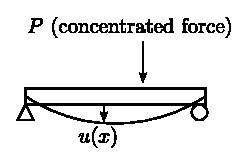
\includegraphics[scale=1.8]{figure/chapter4/4-1-1.eps}
%\caption{\label{fig:blue_rectangle} Rectangle}
\end{figure}
i.e. 
\[
Lw(x;y) = \delta(x-y)
\]
$w(x,y)$ is called the fundamental solution to the operator $L$\\
Consider an inhomogeneous linear differential equation
\begin{equation}
Lu(x) = f(x)
\label{eq: 4-2-3}
\end{equation}
The solution to \eqref{eq: 4-2-3} is
\begin{equation}
u(x) = \int_{-\infty}^\infty \underbrace{w(x;y)}_{
\begin{subarray}{c}
  \text{Kernal function}\\
  \text{transfer function}\\
  \text{influence function}
\end{subarray}
}f(y)dy
\label{eq: 4-2-3}
\end{equation}
\begin{proof}\mbox{}\\
from \eqref{eq: 4-2-3}
\begin{align*}
Lu(x)
&= L\int_{-\infty}^\infty w(x;y)f(y)dy \\
&= \int_{-\infty}^\infty \left[Lw(x;y)\right]f(y)dy \\
&= \int_{-\infty}^\infty \delta(x-y) f(y)dy =f(x)\\
\end{align*}
\[
\Longrightarrow Lw(x;y) = \delta(x-y)
\]
$w(x,y)$ is the \emph{response} of the system $L$ to an impulse input at $x=y$
\begin{figure}[H]
\centering
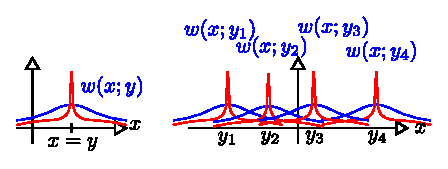
\includegraphics[scale=1.8]{figure/chapter4/4-1-2.eps}
%\caption{\label{fig:blue_rectangle} Rectangle}
\end{figure}
\end{proof}
\item Fundamental Solution to the Laplace equation\\
Consider
\begin{equation}
\nabla^2\phi = \delta(r)
\label{eq: 4-2-4}
\end{equation}
In spherical coordinate with spherical symmetry
\[
\nabla^2\equiv\frac{1}{r^2}\frac{\partial}{\partial r}\left(r^2\frac{\partial}{\partial r}\right)
\]
Guess $\displaystyle\phi = \frac{A}{r}$, $\nabla^2\phi = 0$ everywhere except at $r=0$ where $\phi$ is \emph{undefined} at $r=0$\\
Use integral definition of divergence
\[
\nabla^2\left(\frac{A}{r}\right)_{r=0}=\nabla\cdot\left(\nabla\frac{A}{r}\right)_{r=0} = \lim_{\Delta\volume\to 0}\frac{1}{\Delta\volume}\oiint_{\Delta S}\left(\nabla\frac{A}{r}\right)\cdot\mathbf{n}dS
\]
choose $\Delta\volume$ to be a sphere with radius $\epsilon\to 0$, then 
\[
\nabla\frac{A}{r} = -\frac{A}{r^2}\mathbf{e_r}
\]
and
\begin{align*}
\nabla^2\left(\frac{A}{r}\right)_{r=0}
&= \lim_{\Delta\volume\to 0}\frac{1}{\Delta\volume}\oiint_{\Delta S}-\frac{A}{r^2}\mathbf{e_r}\cdot\mathbf{n}dS \\
&= \lim_{\epsilon\to 0}\frac{-A}{\frac{4}{3}\pi\epsilon^3}\oiint_{\Delta S}\frac{1}{r^2}\underbrace{dS}_{=r^2\sin\theta d\theta d\varphi}\\
&= \lim_{\epsilon\to 0}\frac{-A}{\frac{4}{3}\pi\epsilon^3}\oiint_{\Delta \Omega}\frac{1}{r^2}\underbrace{r^2d\Omega}_{dS} \\
&= \lim_{\epsilon\to 0}\frac{-4\pi A}{\frac{4}{3}\pi\epsilon^3} \to \infty
\end{align*}
i.e., $\displaystyle\nabla^2\left(\frac{A}{r}\right)$ behaves like $\delta(r)$.\\
What is $A$?\\
Recall 
\[
{\oiint \hspace{-23.5pt} \int}_{\volume(\infty)}\delta(r)d\volume\equiv 1, {\oiint \hspace{-23.5pt} \int}_{\volume(\epsilon)}\delta(r)d\volume= 1
\]
but 
\[
{\oiint \hspace{-23.5pt} \int}_{\volume(\infty)}\nabla^2\left(\frac{A}{r}\right)d\volume\equiv{\oiint \hspace{-23.5pt} \int}_{\volume(\epsilon)}\nabla^2\left(\frac{A}{r}\right)d\volume = \nabla^2\left(\frac{A}{r}\right)_{r=0}\underbrace{\volume(\epsilon)}_{\frac{4}{3}\pi\epsilon^3} = 1
\]
\[
\Longrightarrow A = -\frac{1}{4\pi}
\]
i.e. solution to \eqref{eq: 4-2-4} is 
\begin{equation}
\boxed{\phi = -\frac{1}{4\pi r}}\text{ (fundamental solution)}
\label{eq: 4-2-5}
\end{equation}
\begin{exercise}{Show that 2D fundamental solution to the Laplace equation is}
\[
\boxed{\phi = \frac{1}{2\pi}\ln r}
\]
\end{exercise}
\end{itemize}
\subsection{Green's Theorem (Green's Identities) (Green's Formula)}
\begin{itemize}
\item Green's 2\textsuperscript{nd} identity
\begin{equation}
{\oiint \hspace{-23.5pt} \int}_{\volume}\left(\phi'\nabla^2\phi-\phi\nabla^2\phi'\right)d\volume = \oiint_S\left(\phi'\frac{\partial\phi}{\partial n} - \phi\frac{\partial\phi'}{\partial n}\right)dS
\label{eq: 4-2-6}
\end{equation}
both $\phi$ and $\phi'$ are continuous and differentiable scalar function.
\item Application of Green's Theorem\\
Use Green's theorem to express $\phi$ in $\volume$, which satisfies $\nabla^2\phi = 0$, in terms of boundary data on $S$. (This is equivalent to solve $\nabla^2\phi = 0$ in $\volume$ with B.C.'s, $\displaystyle\frac{\partial \phi}{\partial n},\phi$ on $S$.)\\
Let $\phi' = 1/r$, the $\nabla^2\phi' = 0$ everywhere except at $r=0$.\\
Hence
\[
{\oiint \hspace{-23.5pt} \int}_{\volume}\phi'\nabla^2\phi d\volume \vc{=}{\text{if}}{\nabla^2\phi =0} 0, 
\]
\[
{\oiint \hspace{-23.5pt} \int}_{\volume}\phi\nabla^2\phi'\equiv{\oiint \hspace{-23.5pt} \int}_{\volume}\phi\nabla^2\left(\frac{1}{r}\right)d\volume \neq 0\text{ if the point $r=0$ is inside $\volume$}
\]
Recall that
\[
{\oiint \hspace{-23.5pt} \int}_{\volume}\underbrace{\nabla^2\left(-\frac{1}{4\pi r}\right)}_{\sim\delta (r)}d\volume\equiv 1
\]
\[
\therefore{\oiint \hspace{-23.5pt} \int}_{\volume}\phi\nabla^2\left(\frac{1}{r}\right)d\volume = -4\pi{\oiint \hspace{-23.5pt} \int}_{\volume}\phi\underbrace{\nabla^2\left(-\frac{1}{4\pi r}\right)}_{\sim\delta(r)}d\volume = -4\pi\phi_0
\]
where $\phi_0$ is the value of $\phi$ at $r = 0$\\
and
\begin{equation}
\eqref{eq: 4-2-6}\Longrightarrow\oiint_S\left[\frac{1}{r}\frac{\partial\phi}{\partial n} - \phi\frac{\partial}{\partial n}\left(\frac{1}{r}\right)\right]dS
\text{(Green's formula)}
\label{eq: 4-2-7}
\end{equation}
Given $\frac{\partial\phi}{\partial n}, \phi$ on $S$, \eqref{eq: 4-2-7} gives $\phi_0$ at any point in $\volume$.\\
In practice, the use of \eqref{eq: 4-2-7} is 
\begin{tikzpicture}
    % Axes
    \draw [arrows = {-Latex[color=black, fill=white, length=3mm]}] (0,0,0) -- (2,0,0) node [at end, right] {$x$};
    \draw [arrows = {-Latex[color=black, fill=white, length=3mm]}] (0,0,0) -- (0,2,0) node [at end, left] {$y$};
    \draw [arrows = {-Latex[color=black, fill=white, length=3mm]}] (0,0,0) -- (0,0,2) node [at end, left] {$z$};
    \draw[-](3, 3) ellipse (3cm and 2cm);
    \draw [-{Latex[length=2mm]}, rotate=0] (0,0) -- (3,4) node[above]{$P$} node[pos=0.7, anchor=east] {$\mathbf{r_p}$};
    \draw [-{Latex[length=2mm]}, rotate=0] (0,0) -- (2,4.5) node[pos=0.7, anchor=east] {$\mathbf{r'}$};
\end{tikzpicture}
\begin{equation}
4\pi\phi_P = \oiint_S\left[\frac{1}{r}\frac{\partial\phi}{\partial n} - \phi\frac{\partial}{\partial n}\left(\frac{1}{r}\right)\right]dS
\label{eq: 4-2-8}
\end{equation}
where $\displaystyle r = \frac{1}{\abs{\mathbf{r'}-\mathbf{r_p}}}$
\begin{exercise}{For 2D case}
\begin{equation}
-2\pi\phi_P = \oint_C\left[\ln\frac{\partial\phi}{\partial n} - \phi\frac{\partial}{\partial n}\left(\ln r\right)\right]dl
\label{eq: 4-2-9}
\end{equation}
\end{exercise}
\end{itemize}
\newpage
\paragraph*{Modification for the problem involving a solid-body moving in infinite domain (Neumann Exterior Boundary)}
\begin{tikzpicture}
    \filldraw[color=blue!60, fill=blue!10, tangent=0.1](0, 0) ellipse (1cm and 0.5cm);
    \draw[color=blue!60, pattern=hatch, pattern color=blue!60, hatch size=10pt, hatch angle=0](0,0) ellipse (1cm and 0.5cm);
    \draw [blue, ultra thick, use tangent, -latex] (0,0) -- (0,0.7) node [pos=0.7, anchor=east] {$\mathbf{n_S}$};
    \node[blue, ultra thick, below left ] at ($(0,0)$){$\mathbf{\volume_S}$};
    \draw[color=blue!60, tangent=0.4](0, 0) ellipse (5cm and 4cm);
    \draw [blue, ultra thick, use tangent, -latex] (0,0) -- (0,-2) node [pos=1.0, anchor=east] {$\mathbf{n_{\Sigma}}$};
    \filldraw [color=red, fill=red] (3,-1) circle (0.1) node [below right] at  ($(3,-1)$){$P$} ;
    \coordinate (P') at ($(0,0)+(-110:5 and 4)$) ;
    \draw[color=red, -{Latex[length=2mm]}, rotate=0] ($(3,-1)$) -- (P') node [pos=0.5, anchor=south] {$\mathbf{R}$};
    \coordinate (P'') at ($(0,0)+(-70:1 and 0.5)$) ;
    \draw[color=red, -{Latex[length=2mm]}, rotate=0] ($(3,-1)$) -- (P'') node [pos=0.5, anchor=south] {$\mathbf{r}$};
    \draw[transparent, tangent=0.1](0, 0) ellipse (1cm and 0.5cm);
    \draw [blue, ultra thick, use tangent, -latex] (0,0) -- (0,-0.7) node [pos=1.0, anchor=east] {$\mathbf{n = -n_S}$};
    \filldraw [color= yellow!80!black, fill=yellow!80!black, rotate around={-60:(3,1)}] (3,1) rectangle (2,0.5) node [color = yellow!70!black, pos=1.0, anchor=east] {$d\Sigma$};
    \draw[color=yellow!70!black, ultra thick, -{Latex[length=2mm]}, rotate around={-60:(3,1)}] (2.5,0.7) -- (2.5,2) node [pos = 1.0, anchor=south] {$\mathbf{n_\Sigma}$};
    \draw [color=blue!60, -{Latex[length=2mm]}, rotate=0] ($(4,0)$) arc [start angle=-190, end angle=-350, x radius=1.0cm, y radius=0.6cm] node [below] {$\Sigma$};
    \draw [color=blue!60, -{Latex[length=2mm]}, rotate=0] ($(0,0.2)$) arc [start angle=10, end angle=170, x radius=1.0cm, y radius=0.6cm] node [below] {$S$};
\end{tikzpicture}

Consider $\nabla^2\phi = 0$ and $\phi\to\phi_\infty$ as $R\to\infty$ or $\displaystyle\nabla\phi\to 0\left(\nabla\phi\sim o\left(\frac{1}{R^2}\right)\right)$\\
\eqref{eq: 4-2-8} is modified to 
\begin{equation}
\begin{aligned}
4\pi\phi_P
&= \oiint_S\left[\frac{1}{r}\frac{\partial\phi}{\partial n_S} - \phi\frac{\partial}{\partial n_S}\left(\frac{1}{r}\right)\right]dS \\
&+ \oiint_\Sigma\left[\frac{1}{R}\frac{\partial\phi}{\partial n_\Sigma} - \phi\frac{\partial}{\partial n_\Sigma}\left(\frac{1}{R}\right)\right]
\end{aligned}
\tag{$\ast$}
\label{eq: 4-2-9-*}
\end{equation}
Choose $\Sigma$ to be a large sphere with radius $R\to\infty$
\[
\oiint_\Sigma\frac{1}{R}\frac{\partial\phi}{\partial n_\Sigma}d\Sigma = \iint\frac{1}{R}\frac{\partial\phi}{\partial R}\underbrace{R^2\sin\theta d\theta d\varphi}_{d\Sigma}\to 0\text{ as }R\to \infty
\]
\begin{align*}
\oiint_\Sigma\phi\frac{\partial}{\partial n_\Sigma}\left(\frac{1}{R}\right)d\Sigma
&= \oiint_\Sigma\phi\frac{\partial}{\partial R}\left(\frac{1}{R}\right)d\Sigma \\
&= - \oiint_\Sigma \frac{\phi}{R^2} \underbrace{d\Sigma}_{=R^2d\Omega} = -\oiint_\Omega \phi d\Omega = -4\pi \phi_\infty
\end{align*}
Hence
\begin{equation}
\begin{aligned}
\eqref{eq: 4-2-9-*} \Longrightarrow
4\pi\left(\phi_P-\phi_\infty\right)
&= \oiint_S\left[\frac{1}{r}\frac{\partial\phi}{\partial n_S} - \phi\frac{\partial}{\partial n_S}\left(\frac{1}{r}\right)\right]dS \\
&= \oiint_S\left[-\frac{1}{r}\frac{\partial\phi}{\partial n} + \phi\frac{\partial}{\partial n}\left(\frac{1}{r}\right)\right]dS
\end{aligned}
\label{eq: 4-2-10}
\end{equation}
\begin{exercise}{For 2D case}
\begin{equation}
-2\pi\left(\phi_P-\phi_\infty\right) = \oint_C\left[-\ln r\frac{\partial\phi}{\partial n} + \phi\frac{\partial}{\partial n}\left(\ln r\right)\right]dl
\end{equation}
\end{exercise}
\begin{itemize}
\item Interpretation of \eqref{eq: 4-2-10}\\
Let us identity $\phi$ with the velocity potential function $\Phi$
\[
\nabla^2\Phi = 0
\]
Imagine the solid body is replaced by another potential flow with velocity potential $\hat{\Phi}$
\[
\boxed{\nabla^2\hat{\Phi} = 0}
\]
\begin{equation}
\begin{aligned}
&\oiint_S\left[\frac{1}{r}\frac{\partial\hat{\Phi}}{\partial n} - \hat{\Phi}\frac{\partial}{\partial n}\left(\frac{1}{r}\right)\right]dS \\ 
= &{\oiint \hspace{-23.5pt} \int}_{\volume_S}\left[\frac{1}{r}\cancelto{0}{\nabla^2\hat{\Phi}}-\hat{\Phi}\cancelto{0}{\nabla^2\left(\frac{1}{r}\right)}\right]d\volume
\end{aligned}
\label{eq: 4-2-11}
\end{equation}
From \eqref{eq: 4-2-10} + \eqref{eq: 4-2-11}
\begin{equation}
\begin{aligned}
\Longrightarrow
&4\pi\left(\Phi_P-\Phi_\infty\right) \\ = &\oiint_S\left[\left(\Phi - \hat{\Phi}\right)\frac{\partial}{\partial n}\left(\frac{1}{r}\right) + \frac{1}{r}\left(\frac{\partial\hat{\Phi}}{\partial n} - \frac{\partial\Phi}{\partial n}\right)\right]dS
\end{aligned}
\label{eq: 4-2-12}
\end{equation}
Since $\hat{\Phi}$ can be any potential flow, in 2 choice
\begin{enumerate}[label = (\alph*)]
\item If $\hat{\Phi} = \Phi$ on $S$ (but $\displaystyle\frac{\partial \hat{\Phi}}{\partial n}\neq\frac{\partial\Phi}{\partial n}$ on $S$)\\
$\eqref{eq: 4-2-11}\Longrightarrow$
\begin{equation}
\begin{aligned}
4\pi\left(\Phi_P-\Phi_\infty\right) &= \oiint_S\frac{\displaystyle\left(\frac{\partial\hat{\Phi}}{\partial n} - \frac{\partial\Phi}{\partial n}\right)}{r}dS\\ &= \oiint_S\frac{A(S)}{r}dS
\end{aligned}
\label{eq: 4-2-13}
\end{equation}
$A(S)dS\equiv$ strength of the distributed source/sink over $dS$\\
e.g. Panel method
\begin{figure}[H]
\centering
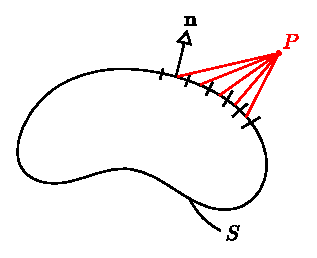
\includegraphics[scale=1.8]{figure/chapter4/4-1-3.eps}
%\caption{\label{fig:blue_rectangle} Rectangle}
\end{figure}
\item If $\displaystyle\frac{\partial \hat{\Phi}}{\partial n}=\frac{\partial\Phi}{\partial n}$ on $S$\\
$\eqref{eq: 4-2-11}\Longrightarrow$
\begin{equation}
\begin{aligned}
4\pi\left(\Phi_P-\Phi_\infty\right) &= \oiint_S\left(\Phi-\hat{\Phi}\right)\frac{\partial}{\partial n}\left(\frac{1}{r}\right)dS \\
&= \oiint_SB(S)\frac{\partial}{\partial n}\left(\frac{1}{r}\right)dS
\end{aligned}
\label{eq: 4-2-14}
\end{equation}
\end{enumerate}
\end{itemize}
\subsection{Irrotational Motion and Circulation}
Irrotational (i.e. $\nabla\times\mathbf{v}=\mathbf{0}\xcancel{\Longrightarrow}\Gamma_C(\equiv\oint_C\mathbf{v}\cdot\mathbf{t}dl)\footnotemark =0$ in $R$ everywhere)\footnotetext{around any circuit $C$ in $R$}\\
\begin{center}
\begin{tikzpicture} 
    \filldraw[color=blue!60, fill=blue!10](0,0) ellipse (1cm and 0.5cm);
    \draw[color=blue!60, pattern=hatch, pattern color=blue!60, hatch size=10pt, hatch angle=0](0,0) circle (1cm and 0.5cm);
    \draw [-{Latex[length=2mm]}, rotate=0] (1.5,0) arc [start angle=-20, end angle=350, x radius=1.5cm, y radius=1.2cm] node [above right] {$C$} node [below right] {$\Gamma_C\neq 0$};
    \draw [-{Latex[length=2mm]}, rotate=0] (3,-2) arc [start angle=-20, end angle=350, x radius=0.7cm, y radius=0.5cm] node [below right] {$\Gamma_C = 0$};
\end{tikzpicture}
\end{center}
\subsubsection{Some Topological Notions}
\begin{itemize}
\item Connectivity\\
A region $R$ is said to be \emph{connected} if any two points in $R$ can be connected by a continuous curve that does not leave $R$.\\
%----------------------
\begin{minipage}{0.4\textwidth}
\begin{tikzpicture} 
    \draw[thick](0,0) circle (1cm and 0.5cm) node [right] {$R$};
    \node at (1.5,0) {$R'$};
    \draw  ($(0,0)+(-70:1 and 0.5)$) .. controls +(down:2mm) and +(left:1mm) .. (1,-0.8) node[right]{$S$} ;
\end{tikzpicture}
\end{minipage} \hfill
\begin{minipage}{0.4\textwidth}
\begin{align*}
R&\colon\text{ connected}\\
R'&\colon\text{ connected}\\
R\cup R'\setminus S&\colon\text{ not a connected region}\\
\end{align*}
\end{minipage}\\
%----------------------
\item Reducible and irreducible circuits\\
If a circuit can be continuously contracted to a point without ever leaving $R$, the circuit is said to be reducible, otherwise, irreducible.\\
In 3D\\
%----------------------
\begin{minipage}{0.4\textwidth}
\begin{tikzpicture} 
    \filldraw[color=blue!60, fill=blue!10](0,0) ellipse (1cm and 0.5cm);
    \draw[color=blue!60, pattern=hatch, pattern color=blue!60, hatch size=10pt, hatch angle=0](0,0) circle (1cm and 0.5cm);
    \draw [thick,-, rotate=0] (1.5,0) arc [start angle=-20, end angle=350, x radius=1.5cm, y radius=1.2cm] node [above right] {$C_2$};
    \draw [thick,-, rotate=0] (4,0) arc [start angle=-20, end angle=350, x radius=0.7cm, y radius=0.5cm] node [below right] {$C_1$};
\end{tikzpicture}
\end{minipage} \hfill
\begin{minipage}{0.4\textwidth}
\begin{align*}
C_1&\colon\text{ reducible}\\
C_2&\colon\text{ reducible}
\end{align*}
\end{minipage}\\
%----------------------
In 2D\\
%----------------------
\begin{minipage}{0.4\textwidth}
\begin{tikzpicture} 
    \filldraw[color=blue!60, fill=blue!10](0,0) ellipse (1cm and 0.5cm);
	\draw[color=blue!60, pattern={Lines[angle=45,distance=5pt]}, pattern color=blue!60](0,0) circle (1cm and 0.5cm);
    \draw [thick,-, rotate=0] (1.5,0) arc [start angle=-20, end angle=350, x radius=1.5cm, y radius=1.2cm] node [above right] {$C_2$};
    \draw [thick,-, rotate=0] (4,0) arc [start angle=-20, end angle=350, x radius=0.7cm, y radius=0.5cm] node [below right] {$C_1$};
\end{tikzpicture}
\end{minipage} \hfill
\begin{minipage}{0.4\textwidth}
\begin{align*}
C_1&\colon\text{ reducible}\\
C_2&\colon\text{ irreducible}
\end{align*}
\end{minipage}\\
%----------------------
In 3D (torus)\\
%----------------------
\begin{minipage}{0.4\textwidth}
\begin{tikzpicture}
\begin{scope}[rotate=0]
%draw right C3
    \draw[thick,-, rotate=0] (1.5,0) [partial ellipse=60:185:0.6cm and 1.4cm];
    \draw[thick,dashed,-, rotate=0] (1.5,0) [partial ellipse=185:250:0.6cm and 1.4cm];
    \draw[thick,-, rotate=0] (1.5,0) [partial ellipse=250:300:0.6cm and 1.4cm] node [below right] {$C_3$};
    \draw[thick,dashed,-, rotate=0] (1.5,0) [partial ellipse=300:420:0.6cm and 1.4cm];
    \draw[thick,-, rotate=0] (-1.9,0) [partial ellipse=60:300:0.6cm and 1.4cm] node [below]{$C_2$};
    \draw[thick,dashed,-, rotate=0] (-1.9,0) [partial ellipse=300:420:0.6cm and 1.4cm];
    \draw [thick,-, rotate=0] (5,0) arc [start angle=-20, end angle=350, x radius=0.7cm, y radius=0.5cm] node [below right] {$C_1$};
    % \draw[thick,-, rotate=0] (-1.9,0) [partial ellipse=360:365:0.6cm and 1.4cm];
    \draw (0,0) ellipse (3 and 1.5);
    \clip (0,-1.8) ellipse (3 and 2.5);
    \draw (0,2.2) ellipse (3 and 2.5);
    \clip (0,2.2) ellipse (3 and 2.5);
    \draw (0,-2.2) ellipse (3 and 2.5);
\end{scope}
\end{tikzpicture}
\end{minipage} \hfill
\begin{minipage}{0.4\textwidth}
\begin{align*}
C_1&\colon\text{ reducible}\\
C_2&\colon\text{ reducible}\\
C_3&\colon\text{ irreducible}
\end{align*}
\end{minipage}\\
%----------------------
\item Simply-Connected Region (SCR)\\
A connected region in which all circuit are reducible.
\item Doubly-Connected Region (DCR)\\
%----------------------
\begin{minipage}{0.2\textwidth}
\begin{tikzpicture} 
    \filldraw[color=blue!60, fill=blue!10](0,0) ellipse (1cm and 0.5cm);
    \draw[color=blue!60, pattern={Lines[angle=45,distance=5pt]}, pattern color=blue!60](0,0) circle (1cm and 0.5cm);
    \node [below right] at (0.5,-0.5){$R$};    
\end{tikzpicture}
\end{minipage} \hfill
\begin{minipage}{0.45\textwidth}
\begin{tikzpicture} 
\begin{scope}[rotate=30]
\node[cylinder, 
    draw = violet, 
    text = purple,
    cylinder uses custom fill, 
    cylinder body fill = magenta!10, 
    cylinder end fill = magenta!40,
    aspect=1.5, rotate=30,
    minimum height=5cm, minimum width=1cm] (c) at (0,0) {};
    \draw[thick,-, rotate=0] (1.5,0) [partial ellipse=25:335:0.6cm and 1.3cm];
\draw[thick,dashed,-, rotate=0] (1.5,0) [partial ellipse=335:385:0.6cm and 1.3cm] ;
\draw[thick, ->] (-2,0)--(-4,0) node[above left] {$-\infty$};
\draw[thick, ->] (2.5,0)--(4.5,0) node[above] {$-\infty$};
\end{scope}
\coordinate (C) at ($(1.5,0)+(250:0.6 and 1.3)$);
\node[below] at (C) {$C\rightarrow$ reducible};
\end{tikzpicture}
\end{minipage}\\
%----------------------
Can render DCR into SCR\\
%----------------------
\begin{minipage}{0.2\textwidth}
\begin{tikzpicture}
    \filldraw[color=blue!60, fill=blue!10, tangent=0.6](0, 0) ellipse (1cm and 0.5cm);
    \draw[color=blue!60, pattern={Lines[angle=45,distance=5pt]}, pattern color=blue!60](0,0) ellipse (1cm and 0.5cm);
    \coordinate (P) at ($(0, 0) + (20:1cm and 0.5cm)$);
    \coordinate (P') at ($(0, 0) + (30:1cm and 0.5cm)$);
    \coordinate (Q) at ($(0, 0) + (20:3cm and 2cm)$);
    \coordinate (Q') at ($(0, 0) + (30:3cm and 2cm)$);
    \coordinate (I) at ($(0, 0) + (25:3cm and 2cm)$);
    \coordinate (I') at ($(0, 0) + (25:6cm and 4cm)$);
    \draw[color=blue!60,-{Stealth[length=2mm]}, rotate=0] (0,0) [partial ellipse=30:150:3cm and 2cm] node[left]{$R(DCR)$};
    \draw[color=blue!60,-{Stealth[length=2mm]}, rotate=0] (0,0) [partial ellipse=150:270:3cm and 2cm];
    \draw[color=blue!60,-{Stealth[length=2mm]}, rotate=0] (0,0) [partial ellipse=270:380:3cm and 2cm];
    \draw[color=blue!60,->-=.5] (P') to  (Q');
    \draw[color=blue!60,->-=.5] (Q) to  (P) ;
    \draw[color=blue!60,-{Stealth[length=2mm]}, rotate=0] (0,0) [partial ellipse=20:-100:1cm and 0.5cm] ;
    \draw[color=blue!60,-{Stealth[length=2mm]}, rotate=0] (0,0) [partial ellipse=-100:-220:1cm and 0.5cm] ;
    \draw[color=blue!60,-{Stealth[length=2mm]}, rotate=0] (0,0) [partial ellipse=-220:-330:1cm and 0.5cm];
    \draw[arrows = {-Latex[color=black, fill=white, length=3mm]}] (I) -- (I') node [above]{$\infty$};
\end{tikzpicture}
\end{minipage} \hfill
\begin{minipage}{0.3\textwidth}
$R\setminus \text{cut}\colon SCR$
\end{minipage}\\
%----------------------
\end{itemize}
\subsubsection{Irrotational Motion and Circulation}
\begin{itemize}
\item In a SCR\\
For any circuit $C$ in SCR $R$,
\[
\Gamma_C = \oint_C\mathbf{v}\cdot\mathbf{t}dl\vc{=}{\text{Stokes'}}{\text{Thm.}}\iint_S\boldsymbol{\xi}\cdot\mathbf{n}dS = 0\text{ since }\boldsymbol{\xi} = \mathbf{0}
\]
hence irrotational flow ($\boldsymbol{\xi}=\mathbf{0}$ everywhere in $R$)
\[
\Longleftrightarrow\Gamma = 0\text{ around any circuit in }R
\]
Further since $\mathbf{v} = \nabla\Phi$
\[
\Gamma_C = \oint_C\mathbf{v}\cdot\mathbf{t}dl = \oint\underbrace{dl\mathbf{t}}_{d\mathbf{r}}\cdot\nabla\Phi = \oint_Cd\Phi = \Phi_{P'} - \Phi_{P} = 0
\]
$\Longrightarrow\Phi$ is a single-valued function.\\
\begin{discussion}\mbox{}\\
The irrotational motion of a fluid in a SCR is also a motion without any circulation. Also, the velocity potential $\Phi$ is single-valued.
\end{discussion}
\item In a DCR\\
\begin{tikzpicture}
    \filldraw[color=blue!60, fill=blue!10, tangent=0.6](0, 0) ellipse (1cm and 0.5cm);
    \draw[color=blue!60, pattern={Lines[angle=45,distance=5pt]}, pattern color=blue!60](0,0) ellipse (1cm and 0.5cm);
    \coordinate (P) at ($(0, 0) + (20:1cm and 0.5cm)$);
    \coordinate (P') at ($(0, 0) + (30:1cm and 0.5cm)$);
    \coordinate (Q) at ($(0, 0) + (20:3cm and 2cm)$);
    \coordinate (Q') at ($(0, 0) + (30:3cm and 2cm)$);
    \coordinate (I) at ($(0, 0) + (25:3cm and 2cm)$);
    \coordinate (I') at ($(0, 0) + (25:6cm and 4cm)$);
    \draw[color=blue!60,-{Stealth[length=2mm]}, rotate=0] (0,0) [partial ellipse=30:150:3cm and 2cm];
    \draw[color=blue!60,-{Stealth[length=2mm]}, rotate=0] (0,0) [partial ellipse=150:270:3cm and 2cm] node [below]{$C_2$};
    \draw[color=blue!60,-{Stealth[length=2mm]}, rotate=0] (0,0) [partial ellipse=270:380:3cm and 2cm];
    \draw[color=blue!60,->-=.5] (P') to  (Q') node [left ]{$D_3$};
    \draw[color=blue!60,->-=.5] (Q) to  (P) node [right]{$D_2$} ;
    \draw[color=blue!60,-{Stealth[length=2mm]}, rotate=0] (0,0) [partial ellipse=20:-100:1cm and 0.5cm] ;
    \draw[color=blue!60,-{Stealth[length=2mm]}, rotate=0] (0,0) [partial ellipse=-100:-220:1cm and 0.5cm] node [above]{$C_3$};
    \draw[color=blue!60,-{Stealth[length=2mm]}, rotate=0] (0,0) [partial ellipse=-220:-330:1cm and 0.5cm];
    \draw [color=blue!60,-{Latex[length=2mm]}, rotate=0] (5.5,0) arc [start angle=-20, end angle=350, x radius=1cm, y radius=1cm] node [above right] {$C_1$} node [left] {$S_1$};
\end{tikzpicture}
\begin{enumerate}[label = (\alph*)]
\item For all reducible circuit in a DCR, like $C_1$
\[
\Gamma_{C_1} = \oint_{C_1}\mathbf{v}\cdot\mathbf{t}dl = \oiint_{S_1}\boldsymbol{\xi}\cdot\mathbf{n}dS = 0\text{ since }\boldsymbol{\xi} = \mathbf{0}\text{ in }S_1
\]
\item For irreducible circuit (like $C_2$)
\begin{align*}
\Gamma_{C_2D_2C_3D_3} 
&= \ointctrclockwise_{C_2}\mathbf{v}\cdot\mathbf{t}dl + \cancel{\int_{D_2}\mathbf{v}\cdot\mathbf{t}dl} + \varointctrclockwise_{C_3}\mathbf{v}\cdot\mathbf{t}dl + \cancel{int_{D_3}\mathbf{v}\cdot\mathbf{t}dl} \\
& = \ointctrclockwise_{C_2}\mathbf{v}\cdot\mathbf{t}dl - \ointctrclockwise_{C_3}\mathbf{v}\cdot\mathbf{t}dl = 0
\end{align*}
\[
\Longrightarrow
\ointctrclockwise_{C_2}\mathbf{v}\cdot\mathbf{t}dl = \ointctrclockwise_{C_3}\mathbf{v}\cdot\mathbf{t}dl\text{ i.e. }\Gamma_{C_2} = \Gamma_{C_3}
\]
(may or may not be zero) \\
where $C_2$ and $C_3$ are reducible circuit
\begin{align*}
\Gamma 
&= \oint_C\mathbf{v}\cdot\mathbf{t}dl \\
&= \oint_C\nabla\Phi\cdot\underbrace{\mathbf{t}dl}_{d\mathbf{r}} = \oint_Cd\Phi = \Phi_P'-\Phi_P\neq 0
\end{align*}
\begin{example}{Free-vortex flow}
\begin{tikzpicture}
    \begin{axis}[xmin = -2, xmax= 2, ymin = -2, ymax= 2, axis lines = middle, title={},axis lines=center, axis equal, axis line style={-{Latex[length=2mm]}}, scaled ticks=false,ytick={}, yticklabels={},xtick={}, xticklabels={}]
    \addplot[domain=0.1:10, color=red, samples = 100]{1/x};
    \addplot[domain=-10:-0.1, color=red, samples = 100]{1/x};
    \draw (axis cs: 0, 0) circle [radius=0.4];
    \draw (axis cs: 0, 0) circle [radius=0.8];
    \draw (axis cs: 0, 0) circle [radius=1.2];
    \draw (axis cs: 0, 0) circle [radius=1.6];
    \node[] at (axis cs: 1.5,-1.5) {$\Gamma_C\neq 0$};
    % \draw (axis cs: 1.6, 0) -- (axis cs: 1.6, 0)
    \node[red] at (axis cs: 1.5,1.5) {$\displaystyle v_\theta\sim \frac{1}{r}$};
    % \addplot[blue,thick, domain=-7:0] {0};
\end{axis}
\end{tikzpicture}\\
$\nabla\times\mathbf{v}=\mathbf{0}$ everywhere except at $r=0$ and 
\[
\Phi = C\theta
\]
i.e., $\Phi$ is not a single-valued function, is a multi-valued function.
\end{example}
\end{enumerate}
\end{itemize}
\subsection{Some General Properties of Irrotational Motion in an Ideal Fluid (Potential Flow)}
\subsubsection{For SCR}
Let $\nabla^2\Phi = 0$ at every point in $R$. From $\mathbf{v} = \nabla\Phi$,
$\Gamma_C = 0$ for any circuit $C$ on $R$.
\begin{enumerate}[label = (\arabic*)]
\item\label{ch4-2-4-(1)} Mean-Value Theorem\\
Define average value of $\Phi$, $\bar{\Phi_P}$ over a spherical surface with radius $r$ centred at $P$
\begin{align}
\bar{\Phi_P}
&= \oiint_S\Phi dS/\oiint_SdS\tag{$\ast$} \\
&= \oiint_S\Phi dS/\oint_\Omega r^2d\Omega\nonumber \\
&= \oint_\Omega\Phi r^2d\Omega /4\pi r^2 = \frac{1}{4\pi}\oint_\Omega\Phi d\Omega\tag{$\ast\ast$}
\end{align}
Now
\begin{align*}
\frac{d\bar{\Phi_P}}{dr}
&= \frac{1}{4\pi}\oint_\Omega\frac{\partial\Phi}{\partial r}d\Omega \\
&= \frac{1}{4\pi r^2}\oint_\Omega\frac{\partial\Phi}{\partial r}\underbrace{r^2d\Omega}_{dS} = \frac{1}{4\pi r^2}\oiint_S\underbrace{\frac{\partial\Phi}{\partial n}}_{\mathbf{n}\cdot\nabla\Phi}dS \\
&= \frac{1}{4\pi r^2}{\oiint \hspace{-23.5pt} \int}_{\volume}\underbrace{\nabla\cdot\left(\nabla\Phi\right)}_{\nabla^2\Phi = 0}d\volume \\
&=0
\end{align*}
$\Longrightarrow\bar{\Phi_P}$ is independent of $r$, i.e. $\bar{\Phi_P} = \Phi_P$ , value of $\Phi$ at point $P$.
\item Maximum and Minimum Principles\\
The potential $\Phi$ can neither be a local maximum nor minimum in the interior of region $R$.
\begin{proof}\mbox{}\\
From \ref{ch4-2-4-(1)}
\[
\bar{\Phi_P} = \Phi_P\text{ independent of }r
\]
Now if $\Phi$ has a local maximum (minimum) at $P$, then all $\Phi$ on $S$ are smaller (larger) than $\Phi_P$, i.e.
\[
\Phi >\bar{\Phi_P} = \frac{1}{4\pi}\oint_\Omega\Phi d\Omega\text{ contradict }\bar{\Phi_P} = \Phi_P
\]
\end{proof}
\item Each (Cartesian) component of $\nabla\Phi$ satisfies a Laplace equation.
\begin{proof}
\[
\because\nabla^2\Phi = 0\therefore\frac{\partial\left(\nabla^2\Phi\right)}{\partial x (y)} = 0\Longrightarrow\nabla^2\underbrace{\left(\frac{\partial\Phi}{\partial x(y)}\right)}_{v_x(v_y)} = 0
\]
\end{proof}
\item The component of $\nabla\Phi(\equiv\mathbf{v})$ can neither be a local maximum nor minimum in the interior of $R$.
\item\label{ch4-2-4-(5)} The magnitude of the velocity $\abs{\mathbf{v}}$ cannot be a local maximum in the interior of $R$.
\item Minimum pressure cannot occur in the interior of $R$.
\begin{proof}\mbox{}\\
From \ref{ch4-2-4-(5)} + Bernoulli's equation
\end{proof}
\item 
\begin{multline*}
\underbrace{{\oiint \hspace{-23.5pt} \int}_R\abs{\nabla\Phi}^2d\volume}_{={\iiint}_R\abs{\mathbf{v}}^2d\volume \propto\text{ KE}} = {\oiint \hspace{-23.5pt} \int}_R\left(\nabla\Phi\cdot\nabla\Phi\right)d\volume\\
 = {\oiint \hspace{-23.5pt} \int}_R\left[\underbrace{\nabla\cdot\left(\Phi\nabla\Phi\right) }_{=\mathbf{n}\cdot\left(\Phi\nabla\Phi\right)dS}- \Phi\cancel{\nabla^2\Phi}\right]d\volume
\end{multline*}
Hence if
\begin{align*}
\Phi = 0&&\text{or}&&\frac{\partial\Phi}{\partial n}&&\text{on }S
\end{align*}
\[
\Longrightarrow{\oiint \hspace{-23.5pt} \int}_R\abs{\mathbf{v}}^2d\volume = 0\Longrightarrow\mathbf{v} = \mathbf{0}\text{ everywhere, $\Phi=$ constant in $R$}
\]
\item
\begin{equation}
{\oiint \hspace{-23.5pt} \int}_R\underbrace{\nabla^2\Phi}_{=\nabla\cdot\left(\nabla\Phi\right)} = \oiint_S\mathbf{n}\cdot\nabla\Phi dS = \oiint_S\frac{\partial\Phi}{\partial n} dS = 0
\end{equation}
i.e. the natural B.C. (Neumann problem) $\displaystyle\frac{\partial\Phi}{\partial n}$ on $S$ cannot be arbitrary specified.
\item Minimum Kinetic Energy\\
Among all possible velocity fields satisfying continuity equation and the specified B.C.'s on $S$, the irrotational one has the minimum KE in $R$.
\begin{proof}\mbox{}\\
Let $\mathbf{v}$ be an irrotational flow field in $R$, then $\mathbf{v}=\nabla\Phi$ and $\nabla\cdot\mathbf{v} = 0$. Let $\mathbf{v_1} = \mathbf{v}+\mathbf{v'}$ be another velocity field which also satisfies $\nabla\cdot\mathbf{v_1} = 0$ and $\mathbf{v}_1\equiv\mathbf{v}$ (i.e. $\mathbf{v'}=0$) on the boundary $S$, but $\mathbf{v_1}$ is not irrotational.\\
Let
\begin{align*}
T = \frac{\rho}{2}{\oiint \hspace{-23.5pt} \int}_Rv^2d\volume, && T_1 = \frac{\rho}{2}{\oiint \hspace{-23.5pt} \int}_R v_1^2d\volume
\end{align*}
\begin{align*}
T_1 - T
&= \frac{\rho}{2}{\oiint \hspace{-23.5pt} \int}_R\left(v_1^2-v^2\right)d\volume \\ 
&= \frac{\rho}{2}{\oiint \hspace{-23.5pt} \int}_R\left[\left(\mathbf{v}+\mathbf{v'}\right)\cdot\left(\mathbf{v}+\mathbf{v'}\right) - v^2\right]d\volume \\
&= \frac{\rho}{2}{\oiint \hspace{-23.5pt} \int}_R\left(2\mathbf{v}\cdot\mathbf{v'}+v'^2\right)
\end{align*}
but 
\begin{align*}
{\oiint \hspace{-23.5pt} \int}_R\mathbf{v}\cdot\mathbf{v'}d\volume
&= {\oiint \hspace{-23.5pt} \int}_R\mathbf{v'}\cdot\nabla\Phi d\volume \\ 
&= {\oiint \hspace{-23.5pt} \int}_R\left[\nabla\cdot\left(\Phi\mathbf{v'}\right) - \Phi\cancel{\nabla\cdot\mathbf{v'}}\right] \\
&= \oiint_S\Phi\left(\mathbf{n}\cdot\mathbf{v'}\right)dS = 0\text{ since }\mathbf{v'} = \mathbf{0}\text{ on }S
\end{align*}
\[
\therefore T_1-T = {\oiint \hspace{-23.5pt} \int}_Rv'^2d\volume\geq 0
\]
\end{proof}
\item The solution of the Neumann exterior problem in a \fbox{SCR} is \emph{unique} up tp \emph{an additive constant}. \\
\begin{tikzpicture}
    \filldraw[color=blue!60, fill=blue!10, tangent=0.1](0, 0) ellipse (1cm and 0.5cm);
    \draw[color=blue!60, pattern=hatch, pattern color=blue!60, hatch size=10pt, hatch angle=0](0,0) ellipse (1cm and 0.5cm);
    \draw [blue, ultra thick, use tangent, -latex] (0,0) -- (0,0.7) node [pos=0.7, anchor=west] {$\mathbf{n_S}$};
    \draw [blue, ultra thick, -latex] (0,0) -- (-2,-1) node [left]{$\mathbf{v_S}$};
    \draw[color=blue!60, tangent=0.4](0, 0) ellipse (5cm and 4cm);
    \draw [blue, ultra thick, use tangent, -latex] (0,0) -- (0,-2) node [pos=1.0, anchor=east] {$\mathbf{n_{\Sigma}}$};
    \draw[transparent, tangent=0.1](0, 0) ellipse (1cm and 0.5cm);
    \draw [blue, ultra thick, use tangent, -latex] (0,0) -- (0,-0.7) node [pos=0.9, anchor=east] {$\mathbf{n = -n_S}$};
    \draw [color=blue!60, -{Latex[length=2mm]}, rotate=0] ($(4,0)$) arc [start angle=-190, end angle=-350, x radius=1.0cm, y radius=0.6cm] node [below] {$\Sigma$};
    \draw [color=blue!60, -{Latex[length=2mm]}, rotate=0] ($(0,0.2)$) arc [start angle=10, end angle=170, x radius=1.0cm, y radius=0.6cm] node [below] {$S$};
\end{tikzpicture}\\
\begin{proof}\mbox{}\\
Let $\Phi_1$ and $\Phi_2$ be two solutions to $\nabla^2\Phi = 0$ and $\displaystyle\frac{\partial\Phi_1}{\partial n} = \frac{\partial\Phi_2}{\partial n} = \mathbf{n}\cdot\mathbf{v_S}$ on $S$.\\
Also
\[
\nabla\Phi_1,\nabla\Phi_2\sim o\left(\frac{1}{r^2}\right)\text{ as }r\to\infty\text{ (i.e. on $\Sigma$)}
\]
Let $\Phi'=\Phi_2-\Phi_1$, then $\displaystyle\nabla^2\Phi'=0,\frac{\partial\Phi'}{\partial n} = 0$ on $S$, $\displaystyle\frac{\partial\Phi'}{\partial n_\Sigma}\sim o\left(\frac{1}{r^2}\right)$ on $\Sigma$
\begin{align*}
{\oiint \hspace{-23.5pt} \int}_R\abs{\nabla\Phi'}^2d\volume 
&= \iiint_R\underbrace{\left(\nabla\Phi'\cdot\nabla\Phi'\right)}_{=\nabla\cdot\left(\Phi'\nabla\Phi'\right)-\Phi'\cancel{\nabla^2\Phi'}}d\volume\\
&= \oiint_S\Phi'\mathbf{n_S}\cdot\nabla\Phi'dS + \underbrace{\oiint_\Sigma\Phi'\overbrace{\mathbf{n_\Sigma}\cdot\nabla\Phi'}^{=\frac{\partial\Phi}{\partial n_\Sigma}\sim o\left(\frac{1}{r^2}\right)}\overbrace{ d\Sigma}^{\sim\mathcal{O}\left(\frac{1}{r^2}\right)}}_{\to 0} \\
&= \oiint_S\Phi'\underbrace{\frac{\partial\Phi'}{\partial n_S}}_{=-\frac{\partial\Phi'}{\partial n} = 0}dS = 0
\end{align*}
\[
\Longrightarrow\nabla\Phi'=0\Longrightarrow\Phi'=\text{ constant}\Longrightarrow\Phi_2-\Phi_1 = \text{ constant}
\]
\end{proof}
The conclusion is not \emph{generally true} for a DCR.
\end{enumerate}

\paragraph*{For DCR}
\begin{itemize}
\item All (1)--(6) and (8) are also valid for DCR
\begin{enumerate}[label = (\arabic*)]
\setcounter{enumi}{9}
\item Uniqueness property of solution\\
\begin{tikzpicture}
    \filldraw[color=blue!60, fill=blue!10, tangent=0.2](0, 0) ellipse (1cm and 0.5cm);
    \draw[color=blue!60, pattern={Lines[angle=45,distance=5pt]}, pattern color=blue!60](0,0) ellipse (1cm and 0.5cm);
    \draw [blue, ultra thick, use tangent, -latex] (0,0) -- (0,0.7) node [pos=0.7, anchor=west] {$\mathbf{n_S}$};
    \draw [blue, ultra thick, use tangent, -latex] (0,0) -- (0,-0.7) node [pos=0.9, anchor=east] {$\mathbf{n = -n_S}$};
    \draw [blue, ultra thick, -latex] (0,0) -- (-2,-1) node [left]{$\mathbf{v_S}$};
    \draw[transparent, tangent=0.4](0, 0) ellipse (5cm and 4cm);
    \draw [blue, ultra thick, use tangent, -latex] (0,0) -- (0,-2) node [pos=1.0, anchor=east] {$\mathbf{n_{\Sigma}}$};
    \coordinate (P) at ($(0, 0) + (20:1cm and 0.5cm)$);
    \coordinate (P') at ($(0, 0) + (30:1cm and 0.5cm)$);
    \coordinate (Q) at ($(0, 0) + (20:5cm and 4cm)$);
    \coordinate (Q') at ($(0, 0) + (30:5cm and 4cm)$);
    \node[red, below right] at (P){$D$};
    \node[red, above ] at (P'){$A$};
    \node[red, right] at (Q'){$B$};
    \node[red, right] at (Q){$C$};
    \draw[color=blue!60,-{Stealth[length=2mm]}, rotate=0] (0,0) [partial ellipse=30:150:5cm and 4cm];
    \draw[color=blue!60,-{Stealth[length=2mm]}, rotate=0] (0,0) [partial ellipse=150:270:5cm and 4cm];
    \draw[color=blue!60,-{Stealth[length=2mm]}, rotate=0] (0,0) [partial ellipse=270:380:5cm and 4cm];
    \draw[color=blue!60,->-=.5] (P') to  (Q');
    \coordinate (P'Q'middle) at (4,0.7);  
    \draw [blue, ultra thick, use tangent, -latex] ($(P')!(P'Q'middle)!(Q')$) -- (P'Q'middle) node [below] {$\mathbf{n_+} = \mathbf{n_C}$};
    \draw[color=blue!60,->-=.5] (Q) to  (P);
    \coordinate (PQmiddle) at (1.5,1.5);   
    \draw [blue, ultra thick, use tangent, -latex] ($(P)!(PQmiddle)!(Q)$) -- (PQmiddle) node [above] {$\mathbf{n_-} = -\mathbf{n_C}$};
    \draw[color=blue!60,-{Stealth[length=2mm]}, rotate=0] (0,0) [partial ellipse=20:-100:1cm and 0.5cm];
    \draw[color=blue!60,-{Stealth[length=2mm]}, rotate=0] (0,0) [partial ellipse=-100:-220:1cm and 0.5cm];
    \draw[color=blue!60,-{Stealth[length=2mm]}, rotate=0] (0,0) [partial ellipse=-220:-330:1cm and 0.5cm];
    \node[color=blue!60, above left] at ($(3,-3)$){$R$};
    \draw [color=blue!60, -{Latex[length=2mm]}, rotate=0] ($(0,0.2)$) arc [start angle=10, end angle=170, x radius=1.0cm, y radius=0.6cm] node [below] {$S$};
\end{tikzpicture}\\
Let $\Phi_1$ and $\Phi_2$ be two solutions to $\nabla^2\Phi = 0$ in the region $R$ (DCR) and 
\[
\frac{\partial\Phi_1}{\partial n} = \frac{\partial\Phi_2}{\partial n} = \mathbf{n}\cdot\mathbf{v_S}\text{ on }S
\]
also
\[
\frac{\partial\Phi_1}{\partial n_\Sigma},\frac{\partial\Phi_2}{\partial n_\Sigma}\sim o\left(\frac{1}{r}\right)\text{ as }r\to\infty\text{ (i.e. on $\Sigma$)}
\]
Let $\Phi'=\Phi_2-\Phi_1$, then $\displaystyle\nabla^2\Phi'=0,\frac{\partial\Phi'}{\partial n_S} = 0$ on $S$, $\displaystyle\frac{\partial\Phi'}{\partial n_\Sigma}\sim o\left(\frac{1}{r}\right)$ on $\Sigma$
\begin{align*}
\iint_R\abs{\nabla\Phi'}^2dA_R
&= \iint_R\underbrace{\left(\nabla\Phi'\cdot\nabla\Phi'\right)}_{=\nabla\cdot\left(\Phi'\nabla\Phi'\right)-\Phi'\cancel{\nabla^2\Phi'}}dA_R\\
&= \ointctrclockwise_\Sigma\Phi'\underbrace{\frac{\partial\Phi'}{\partial n_\Sigma}}_{\sim o\left(\frac{1}{r}\right)}\underbrace{dl}_{\sim O(r)} + \varointctrclockwise_S\Phi\cancel{\frac{\partial\Phi}{\partial n_S}}dl \\
&+ \int_A^B\Phi'_+\left(\frac{\partial\Phi'}{\partial n_+}\right)_+dl + \int_C^D\Phi'_-\left(\frac{\partial\Phi'}{\partial n_-}\right)_-dl \\
&= \int_A^B\Phi'_+\left(\frac{\partial\Phi'}{\partial n_+}\right)_+dl + \int_C^D\Phi'_-\left(\frac{\partial\Phi'}{\partial n_-}\right)_-dl \\
&= \int_{\text{cut}}\left(\Phi'_+-\Phi'_-\right)\frac{\partial\Phi'}{\partial n_C}dl \\
&= \int_{\text{cut}}\left[\left(\Phi_2-\Phi_1\right)_+ - \left(\Phi_2-\Phi_1\right)_-\right]\frac{\partial\Phi'}{\partial n_C}dl \\
&= \int_{\text{cut}}\left\{\underbrace{\left[\left(\Phi_2\right)_+ -\left(\Phi_2\right)_-\right]}_{-\Gamma_2} - \underbrace{\left[\left(\Phi_1\right)_+ - \left(\Phi_1\right)_-\right]}_{-\Gamma_1}\right\}\frac{\partial\Phi'}{\partial n_C}dl \\
&= \left(\Gamma_1-\Gamma_2\right)\int_{\text{cut}}\frac{\partial\Phi'}{\partial n_C}dl
\end{align*}
\begin{enumerate}[label = (\roman*)]
\item If $\Gamma_1 = \Gamma_2$, then 
\[
\iint_R\left(\nabla\Phi'\right)\cdot\left(\nabla\Phi'\right)dA_R = 0\Longrightarrow\nabla\Phi' = 0
\]
\[
\Longrightarrow\Phi' = \text{ constant}
\]
\[
\Longrightarrow\Phi_2 = \Phi_1 + \text{ constant}
\]
\item If $\Gamma_1 \neq \Gamma_2$, then 
\[
\Phi_2 \neq \Phi_1 + \text{ in general}
\]
\end{enumerate}
\end{enumerate}
\begin{discussion}\mbox{}\\
In a DCR, the solution to the Neumann exterior problem is unique determined only when the \emph{circulation is specified}. Different circulations gives different solutions.
\end{discussion}
\end{itemize}
\subsection{Flow Induced by Vorticity}
Recall vorticity that $\boldsymbol{\xi} = \nabla\times\mathbf{v}$
\begin{align*}
\text{If }\mathbf{v}(\mathbf{r},t)\text{ is known}&\vc{\Longrightarrow}{\nabla\times\mathbf{v}}{}\boldsymbol{\xi}(\mathbf{r},t) \\
\text{If }\boldsymbol{\xi}(\mathbf{r},t)\text{ is known}&\vc{\Longrightarrow}{?}{}\mathbf{v}(\mathbf{r},t) 
\end{align*}
Note that $\mathbf{v}(\mathbf{r},t)$ thus determined is not unique!
\subsubsection{Biot-Savart Law}
(Calculation of the velocity field induced by vorticity)
\[
\mathbf{v} = \nabla\times\boldsymbol{\Psi}\text{ (from $\nabla\cdot\mathbf{v} = 0$)}
\]
Now
\[
\boldsymbol{\xi} = \nabla\times\mathbf{v} = \nabla\times\left(\nabla\times\boldsymbol{\Psi}\right) = -\nabla^2\boldsymbol{\Psi} + \nabla\left(\nabla\cdot\boldsymbol{\Psi}\right)
\]
As before, without loss of generality can set $\nabla\cdot\boldsymbol{\Psi} = 0$.\\
Hence 
\begin{subequations}
\begin{equation}
\boxed{\nabla^2\boldsymbol{\Psi} = -\boldsymbol{\xi}}
\label{eq: 4-5-1a}
\end{equation}
In component form
\begin{equation}
\nabla^2\Psi_i = -\xi_i
\label{eq: 4-5-1b}
\end{equation}
\end{subequations}
%----------------------
\begin{minipage}{0.4\textwidth}
Recall
\[
Lu(x) = f(x)
\]
\[
\L\underbrace{u(x)}_{w(x;y)} = \delta(x-y)
\]
\[
u(x) = \int w(x;y)f(y)dy
\]
\end{minipage}\hfill
\begin{minipage}{0.4\textwidth}
Recall
\[
\nabla^2\Psi_i = \delta(\abs{\mathbf{r}-\mathbf{r'}})
\]
solution is 
\[
\Psi_{i,\text{FS}}(\mathbf{r};\mathbf{r'}) = -\frac{1}{4\pi\abs{\mathbf{r}-\mathbf{r'}}}
\]
\end{minipage}\\
%----------------------
then the solution to the \eqref{eq: 4-5-1b} is
\begin{align*}
\Psi_i(\mathbf{r},t) 
&= \iiint_{\volume_{r'}}-\xi_i(\mathbf{r'},t)\Psi_{i,\text{FS}}(\mathbf{r};\mathbf{r'}) d\volume_{r'} \\
&= \frac{1}{4\pi}\iiint_{\volume_{r'}}\frac{\xi(\mathbf{r',t})}{\abs{\mathbf{r}-\mathbf{r'}}}d\volume_{r'}
\end{align*}
Sum up all 3 components
\begin{equation}
\boldsymbol{\Psi}(\mathbf{r},t) = \frac{1}{4\pi}\iiint_{\volume_{r'}}\frac{\boldsymbol{\xi}(\mathbf{r'},t)}{\abs{\mathbf{r}-\mathbf{r'}}}d\volume_{r'}
\label{eq: 4-5-2}
\end{equation}
solution to the inhomogeneous \eqref{eq: 4-5-1a}\\
The induced velocity field $\mathbf{v}(\mathbf{r},t)$ is then
\begin{align}
\mathbf{v}(\mathbf{r},t)
&= \nabla\times\boldsymbol{\Psi}\nonumber\\
&= \frac{1}{4\pi}\nabla_r\footnotemark\times\iiint_{\volume_{r'}}\frac{\boldsymbol{\xi}(\mathbf{r'},t)}{\abs{\mathbf{r}-\mathbf{r'}}}d\volume_{r'}\nonumber \\
&= \frac{1}{4\pi}\iiint_{\volume_{r'}}\left[\nabla_r\left(\frac{1}{\abs{\mathbf{r}-\mathbf{r'}}}\right)\times\boldsymbol{\xi}(\mathbf{r'},t)\right]d\volume_{r'}\nonumber \\
&= \frac{1}{4\pi}\iiint_{\volume_{r'}}\frac{\boldsymbol{\xi}(\mathbf{r'},t)\times\mathbf{R}}{R^3}d\volume_{r'}\label{eq: 4-5-3}
\end{align}
where $\mathbf{R} = \mathbf{r} - \mathbf{r'}$ and note that
\[
\nabla_r\times\left(f\boldsymbol{\xi}(\mathbf{r'},t)\right) = \nabla_r f\times\boldsymbol{\xi} + f\cancel{\nabla_r\times\boldsymbol{\xi}(\mathbf{r'},t)}
\]
\footnotetext{Note that the subscript $r$ on the curl to emphasize that the curl is to be taken with respect to the coordinate of the point $\mathbf{r}$.}
\begin{exercise}{Show that}\\
\[
\nabla_r\left(\frac{1}{\abs{\mathbf{r}-\mathbf{r'}}}\right) = - \frac{\mathbf{r}-\mathbf{r'}}{\abs{\mathbf{r}-\mathbf{r'}}^3} = -\frac{\mathbf{R}}{R^3}
\]
\begin{proof}\mbox{}\\
Let $\mathbf{R} = x_i\mathbf{e_i}$ and $R = (x_ix_i)^{1/2}$, then 
\begin{align*}
\nabla\left(R^n\right)
&= \nabla\left(x_ix_i\right)^{n/2} = \mathbf{e_i}\frac{n}{2}\left(x_jx_j\right)^{n/2 -1}2\underbrace{x_{k,i}}_{=\delta_{ki}}x_k \\
&= n\mathbf{e_i}\left(x_jx_j\right)^{\frac{n-2}{2}}x_i = nR^{n-2}\mathbf{R}
\end{align*}
\end{proof}
\end{exercise}
In elemental form
\begin{equation}
d\boldsymbol{\Psi}(\mathbf{r},t) = \frac{1}{4\pi}\frac{\boldsymbol{\xi}(\mathbf{r'},t)d\volume_{r'}}{\abs{\mathbf{r}-\mathbf{r'}}}
\label{eq: 4-5-4}
\end{equation}
\begin{equation}
d\mathbf{v}(\mathbf{r},t) = \frac{1}{4\pi}\frac{\boldsymbol{\xi}(\mathbf{r'},t)d\volume_{r'}\times\mathbf{R}}{\abs{\mathbf{r}-\mathbf{r'}}}
\label{eq: 4-5-5}
\end{equation}
\vspace{8em}
\begin{center}
\begin{tikzpicture}[scale=2,transform canvas]
    % Axes
    \draw [arrows = {-Latex[color=black, fill=white, length=3mm]}] (0,0,0) -- (1,0,0) node [at end, right] {$x$};
    \draw [arrows = {-Latex[color=black, fill=white, length=3mm]}] (0,0,0) -- (0,1,0) node [at end, left] {$y$};
    \draw [arrows = {-Latex[color=black, fill=white, length=3mm]}] (0,0,0) -- (0,0,1) node [at end, left] {$z$};
    % \draw[-](2,1, -1) ellipse (0.7cm and 0.5cm);
    \filldraw[color=blue!60, fill=blue!10, tangent=0.1](2,1, -1) ellipse (0.35cm and 0.25cm);
    \draw[color=blue!60, pattern=hatch, pattern color=blue!60, hatch size=10pt, hatch angle=0](2,1, -1) ellipse (0.35cm and 0.25cm) node [inner sep=10pt, anchor=north west] {$\volume_{r'}$};
    % \draw[-](2,1, -1) ellipse (0.35cm and 0.25cm);
    \draw [-{Latex[length=2mm]}, rotate=0] (0,0, 0) -- (1,2, 1) node[above]{$P$} node[pos=0.8, anchor=east] {$\mathbf{r_p}$};
    \draw [-{Latex[length=2mm]}, rotate=0] (0,0, 0) -- (2,1, -1) node[pos=0.7, anchor=east] {$\mathbf{r'}$};
    \draw [-{Latex[length=2mm]}, rotate=0] (2,1, -1) -- (1,2, 1) node[pos=0.5, anchor=south] {$\mathbf{R}$};
    \draw [-{Latex[length=2mm]}, rotate=0] (2,1, -1) -- (3,2, -1) node[pos=0.9, anchor=south] {$\boldsymbol{\xi}(\mathbf{r},t)$};
    \draw [-{Latex[length=2mm]}, rotate=0] (1,2, 1) -- (0,3, 3) node[pos=0.7, anchor=south] {$d\boldsymbol{v}(\mathbf{r},t)$};
\end{tikzpicture}
\end{center}

\subsubsection{Velocity Induced by Concentrated Vorticity}
\begin{itemize}
\item Single Vortex Filament\\
\begin{figure}[H]
\centering
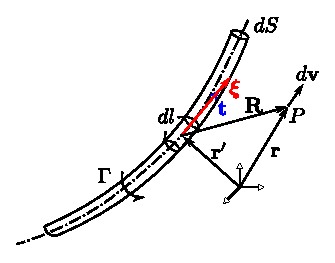
\includegraphics[scale=1.8]{figure/chapter4/4-1-4.eps}
%\caption{\label{fig:blue_rectangle} Rectangle}
\end{figure}
From Helmholtz Theorem
\[
\boldsymbol{\xi}\cdot\mathbf{t}dS = \Gamma = \text{ constant}
\]
From \eqref{eq: 4-5-5}
\begin{equation}
\Longrightarrow
d\mathbf{v}(\mathbf{r}) = \frac{1}{4\pi} \frac{\boldsymbol{\xi}(\mathbf{r'})d\volume_{r'}\times\mathbf{R}}{R^3} \vc{=}{\footnotemark}{} \frac{1}{4\pi}\frac{\Gamma dl\mathbf{t}\times \mathbf{R}}{R^3}
\label{eq: 4-5-6}
\end{equation}
Since $\Gamma$ is constant
\begin{equation}
\mathbf{v}(\mathbf{r}) = \frac{\Gamma}{4\pi}\int\frac{\mathbf{t}\times\mathbf{R}}{R^3}dl
\label{eq: 4-5-7}
\end{equation}
\footnotetext{$\boldsymbol{\xi}(\mathbf{r'})d\volume_{r'} = \boldsymbol{\xi}\left(\mathbf{t}dS\cdot d\mathbf{l}\right) = \boldsymbol{\xi}\left(\mathbf{t}dS\cdot\frac{\boldsymbol{\xi}}{\xi}dl\right) = \boldsymbol{\xi}\frac{\Gamma}{\xi}dl = \Gamma \mathbf{t}dl$}\\
\item Straight Infinite-long vortex filament

\tdplotsetmaincoords{60}{110}
\begin{center}

\begin{tikzpicture}[scale=3, tdplot_main_coords]
    \coordinate (O) at (0,0,0);
    \tdplotsetcoord{inf}{2}{0}{90} 
    \tdplotsetcoord{ninf}{-0.5}{0}{-90} 
    \tdplotsetcoord{P}{2}{30}{70}
    \tdplotsetcoord{l}{0.5}{0}{90} 
    \tdplotsetcoord{dl}{0.8}{0}{90} 
    \tdplotsetcoord{t}{1.1}{0}{90} 
    \draw plot [mark=*, mark size=0.5] (P) node [right] {$P$}; 
    \draw plot [mark=*, mark size=0.5] (l) ; 
    \draw plot [mark=*, mark size=0.5] (t) ; 
	\draw plot [mark=*, mark size=0.5] (O) node [left] {$O$}; 
    \draw[-{Latex[length=2mm]}] (O) -- (inf) node [at end, above]{$\infty$};
    \draw[-{Latex[length=2mm]}] (O) -- (ninf) node [at end, below]{$-\infty$};
    \draw[thick,-{Latex[length=2mm]}] (O) -- (P) node [pos=0.5, anchor=north]{$\mathbf{r}$} ;
    \draw[thick, -{Latex[length=2mm]}] (O) -- (l) node [pos=0.7, anchor=east]{$\mathbf{r'}$} node [pos=0.7, anchor=west]{$l$} ;
    \draw[ {Latex[length=2mm]}-{Latex[length=2mm]}] (l) -- (dl) node [pos=0.5, anchor=east]{$dl$} ;
    \draw[thick, -{Latex[length=2mm]}] (dl) -- (t) node [pos=0.7, anchor=east]{$\mathbf{t}$}  ;
    \draw[thick, -{Latex[length=2mm]}] (l) -- (P) node [pos=0.5, anchor=south]{$\mathbf{R}$} ;

    \draw[-] (P) -- (Pz) node [pos=0.5, anchor=south] {${r_0}$};

	\draw pic["$\alpha$", draw=red, text=red, <->, angle eccentricity=1.2, angle radius=1.6cm] {angle=P--O--l};
	\draw pic["$\theta$", draw=red, text=red, <->, angle eccentricity=1.2, angle radius=1cm] {angle=P--l--inf};
	\coordinate (e) at (-1.8794,0.684,0);
	\draw[thick, -{Latex[length=2mm]}] (P) -- (e) node [right, at end]{$\mathbf{e}$} ;
	\coordinate (v1) at ($(Pz) + (0,0,0.1)$);
	\coordinate (v3) at ($(Pz)!0.2!(P)$);
	\coordinate (v2) at (0.0684,0.18794,1.832);
	\draw [thick, red] (v1) -- (v2) -- (v3);
%	\draw [red] (Pz)  ++(0,0,0.1) -- ($(x)!0.25!(vtip)$)--(a);  
\end{tikzpicture}
\end{center}
\begin{equation}
\mathbf{t}\times\mathbf{R} = R\sin\theta\mathbf{e}
\label{eq: 4-5-8}
\end{equation}
where $\mathbf{e}$ is unit vector into board.\\
From \eqref{eq: 4-5-7}
\begin{align}
\mathbf{v}(\mathbf{r}) 
&= \frac{\Gamma}{4\pi}\int_{-\infty}^\infty\mathbf{e}\frac{\sin\theta}{R^2}dl
\tag{$\ast$}
\label{eq: 4-5-*} \\
&\vc{=}{\text{in this}}{\text{case}}\mathbf{e}\frac{\Gamma}{4\pi}\int_{-\infty}^{\infty}\frac{\sin\theta}{R^2}dl \vc{=}{\footnotemark}{} \mathbf{e}\frac{\Gamma}{4\pi}\int_0^\pi\frac{\sin\theta}{r_0}d\theta\nonumber  \\
&= \frac{\Gamma}{2\pi r_0}\mathbf{e}\label{eq: 4-5-88}
\end{align}
\footnotetext{From geometry, $\displaystyle\frac{r\cos\alpha - l}{r_0} = \cot\theta\Longrightarrow dl = \frac{r_0d\theta}{\sin^2\theta}$ and $\displaystyle R^2 = \frac{r_0^2}{\sin^2\theta}$}
\begin{note}\mbox{}\\
\begin{enumerate}[label = \protect\circled{\arabic*}]
\item For semi-infinite long vortex filament
%----------------------
\begin{minipage}{0.4\textwidth}
\begin{equation}
\mathbf{v}(\mathbf{r}) = \frac{\Gamma}{4\pi r_0}\left(1+\cos\theta_0\right)\mathbf{e}
\label{eq: 4-5-9}
\end{equation}
\[
\left(\int_{\theta = 0}^{\theta = \pi}\left(\cdots\right)d\theta\longrightarrow\int_{\theta = \theta_0}^{\theta = \pi}\left(\cdots\right)d\theta\right)
\]
\end{minipage} \hfill
\begin{minipage}{0.3\textwidth}
\tdplotsetmaincoords{90}{0}
\begin{center}
\begin{tikzpicture}[scale=2, tdplot_main_coords]
    \coordinate (O) at (0,0,0);
    \tdplotsetcoord{inf}{2}{0}{90} 
    \tdplotsetcoord{ninf}{-0.5}{0}{-90} 
    \tdplotsetcoord{P}{2}{30}{70}
    \tdplotsetcoord{l}{0.5}{0}{90} 
    \tdplotsetcoord{dl}{0.8}{0}{90} 
    \tdplotsetcoord{t}{1.1}{0}{90} 
    \draw plot [mark=*, mark size=0.5] (P) node [right] {$P$}; 
	\draw plot [mark=*, mark size=0.5] (O) node [left] {$O$}; 
    \draw[-{Latex[length=2mm]}] (O) -- (inf) node [at end, above]{$\infty$};
    \draw[thick,-{Latex[length=2mm]}] (O) -- (P) node [pos=0.5, anchor=west]{$\mathbf{r}$} ;


    \draw[-] (P) -- (Pz) node [pos=0.5, anchor=south] {${r_0}$};
	\coordinate (v1) at ($(Pz) + (0,0,0.1)$);
	\coordinate (v3) at ($(Pz)!0.2!(P)$);
	\coordinate (v2) at (0.0684,0.18794,1.832);
	\draw [thick, red] (v1) -- (v2) -- (v3);
	\draw pic["$\theta_0$", draw=red, text=red, <->, angle eccentricity=1.6, angle radius=1.6cm] {angle=P--O--Pz};
\end{tikzpicture}
\end{center}
\end{minipage}\\
%----------------------
\item For a segment of vortex filament
%----------------------
\begin{minipage}{0.4\textwidth}
\begin{equation}
\begin{aligned}
\mathbf{v}(\mathbf{r})
&= \frac{\Gamma}{4\pi r_0}\left(\cos\theta_1-\cos\theta_2\right) \\
&= \frac{\Gamma}{4\pi r_0}\left(\cos\theta_1+\cos\theta_3\right)
\end{aligned}
\label{eq: 4-5-9}
\end{equation}
\end{minipage} \hfill
\begin{minipage}{0.3\textwidth}
\tdplotsetmaincoords{90}{0}
\begin{center}
\begin{tikzpicture}[scale=2, tdplot_main_coords]
    \coordinate (O) at (0,0,0);
    \tdplotsetcoord{inf}{2.3}{0}{90} 
    \tdplotsetcoord{ninf}{-0.5}{0}{-90} 
    \tdplotsetcoord{P}{2}{60}{50}
    \tdplotsetcoord{l}{0.5}{0}{90} 
    \tdplotsetcoord{dl}{0.8}{0}{90} 
    \tdplotsetcoord{t}{1.1}{0}{90} 
    \tdplotsetcoord{tt}{1.7}{0}{90} 
    \draw plot [mark=*, mark size=0.5] (P) node [right] {$P$}; 
    \draw plot [mark=*, mark size=0.5] (tt) ; 
	\draw plot [mark=*, mark size=0.5] (O) node [left] {$O$}; 
    \draw[dashed] (tt) -- (inf);
    \draw[-] (O) -- (tt);
    \draw[thick,-{Latex[length=2mm]}] (O) -- (P) node [pos=0.5, anchor=west]{$\mathbf{r}$} ;
	\draw[thick,-{Latex[length=2mm]}] (tt) -- (P) ;

    \draw[-] (P) -- (Pz) node [pos=0.5, anchor=south] {${r_0}$};
	\coordinate (v1) at ($(Pz) + (0,0,0.1)$);
	\coordinate (v3) at ($(Pz)!0.2!(P)$);
	\coordinate (v2) at (0.22266,0.26536,1.1);
	\draw [thick, red] (v1) -- (v2) -- (v3);
	\draw pic["$\theta_1$", draw=red, text=red, <->, angle eccentricity=1.3, angle radius=1.2cm] {angle=P--O--Pz};
	\draw pic["$\theta_3$", draw=red, text=red, <->, angle eccentricity=1.4, angle radius=0.7cm] {angle=O--tt--P};
	\draw pic["$\theta_2$", draw=red, text=red, <->, angle eccentricity=1.3, angle radius=1.2cm] {angle=P--tt--inf};
\end{tikzpicture}
\end{center}
\end{minipage}\\
%----------------------
\end{enumerate}
\end{note}
\item (Concentrated) Horseshoe Vortex filament
\begin{figure}[H]
\centering
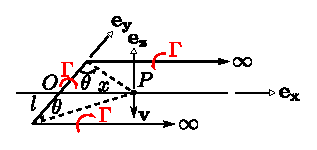
\includegraphics[scale=1.8]{figure/chapter4/4-1-5.eps}
%\caption{\label{fig:blue_rectangle} Rectangle}
\end{figure}
\[
\mathbf{v} = -\mathbf{e_z}\left[\frac{\Gamma}{4\pi x}\left(\cos\theta + \cos\theta\right) + 2\frac{\Gamma}{4\pi l}\left(1+\sin\theta\right)\right]
\]
or
\begin{equation}
\mathbf{v}(x) = -\mathbf{e_z}\frac{\Gamma}{2\pi l}\left[1 + \frac{\sqrt{l^2+x^2}}{x}\right]
\label{eq: 4-5-11}
\end{equation}
\begin{itemize}
\item In thin airfoil theory
\begin{figure}[H]
\centering
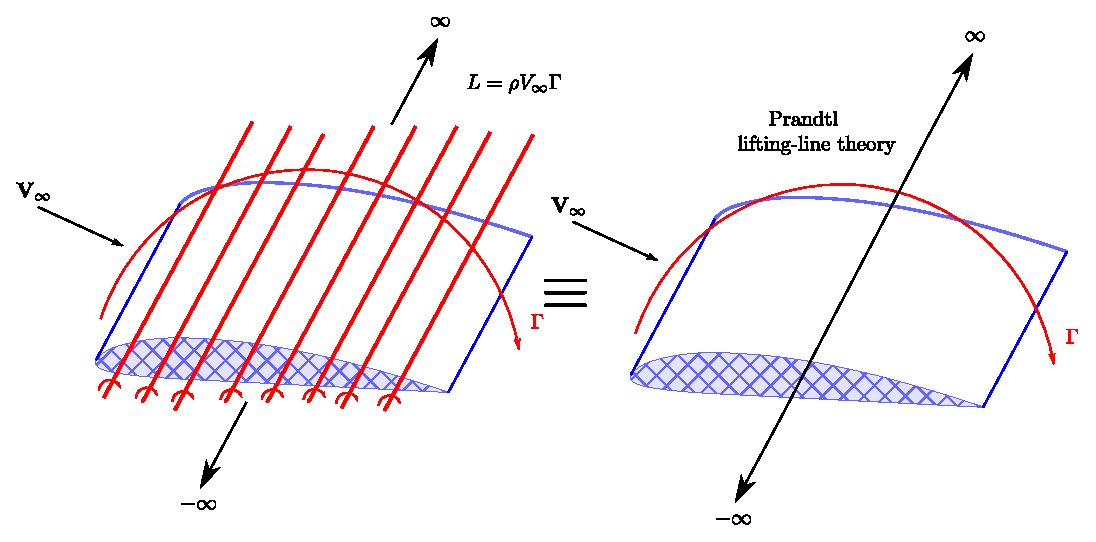
\includegraphics[scale=1.0]{figure/chapter4/4-1-6.eps}
%\caption{\label{fig:blue_rectangle} Rectangle}
\end{figure}
\item In 3D (finite wing)
\begin{figure}[H]
\centering
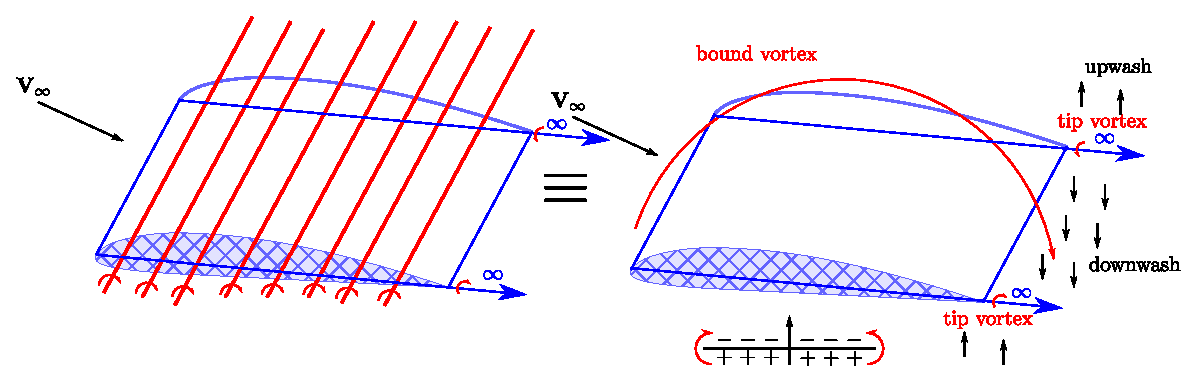
\includegraphics[scale=0.9]{figure/chapter4/4-1-7.eps}
%\caption{\label{fig:blue_rectangle} Rectangle}
\end{figure}
\item In real viscous flow
\begin{figure}[H]
\centering
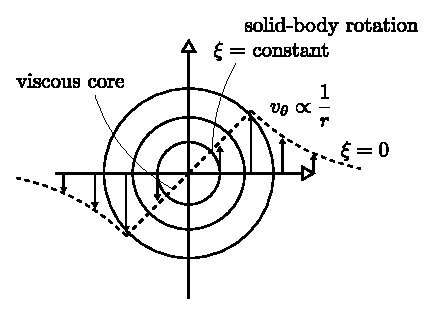
\includegraphics[scale=0.9]{figure/chapter4/4-1-8.eps}
%\caption{\label{fig:blue_rectangle} Rectangle}
\end{figure}
which is Rankine vortex (or Circular vortex). 
\end{itemize}
\end{itemize}
\subsubsection{Velocity Induced by Concentrated Vorticity- Concentrated Vortex Sheet}
%----------------------
\begin{minipage}{0.4\textwidth}
\begin{figure}[H]
\centering
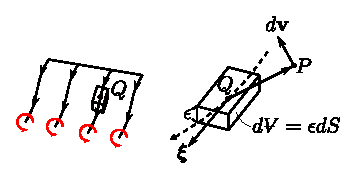
\includegraphics[scale=1.3]{figure/chapter4/4-1-9.eps}
%\caption{\label{fig:blue_rectangle} Rectangle}
\end{figure}
\end{minipage} \hfill
\begin{minipage}{0.5\textwidth}
\[
\boldsymbol{\xi}d\volume = \boldsymbol{\xi}\epsilon dS
\]
as $\epsilon\to 0$, let $\abs{\boldsymbol{\xi}}\to\infty$\\
so that $\abs{\boldsymbol{\xi}\epsilon} = \abs{\boldsymbol{\gamma}}=$ constant at point $Q$
\end{minipage}\\
%----------------------
Biot-Savart law:
\begin{equation}
d\mathbf{v}(\mathbf{r}) = \frac{1}{4\pi}\frac{\boldsymbol{\gamma}(\mathbf{r}')dS\times\mathbf{R}}{R^3}
\label{eq: 4-5-11}
\end{equation}
What is $\abs{\boldsymbol{\gamma}}$?
\begin{figure}[H]
\centering
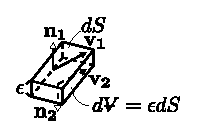
\includegraphics[scale=1.8]{figure/chapter4/4-1-10.eps}
%\caption{\label{fig:blue_rectangle} Rectangle}
\end{figure}
Now
\[
\boldsymbol{\xi}d\volume = \nabla\times\mathbf{v}d\volume\vc{=}{\footnotemark}{}\oiint_{\Delta S}\mathbf{n}\times \mathbf{v}dS
\]
\footnotetext{integral definition of $\nabla\times\mathbf{v}$}
Hence
\begin{align*}
\boldsymbol{\xi}d\volume
&= \lim_{\epsilon\to 0}\boldsymbol{\xi}\epsilon dS\\
&= \lim_{\epsilon\to 0}\oiint_{\Delta S}\mathbf{n}\times\mathbf{v}dS \\
&= \left(\mathbf{n_1}\times\mathbf{v}_1 + \mathbf{n_2}\times\mathbf{v}_2\right)dS
\end{align*}
\[
\Longrightarrow\boldsymbol{\gamma} = \mathbf{n}\times\left(\mathbf{v_1}-\mathbf{v_2}\right)
\]
but $\left(\mathbf{v_1}-\mathbf{v_2}\right)\perp\mathbf{n}$\\
hence
\begin{equation}
\abs{\boldsymbol{\gamma}} = \abs{\mathbf{v_1}-\mathbf{v_2}} = \abs{u_1-u_2}
\label{eq: 4-5-12}
\end{equation}\\
\vspace{5em}
%----------------------
\begin{minipage}{0.4\textwidth}
\begin{tikzpicture}
\begin{scope}[scale=2,transform canvas]
\coordinate (O) at (0,0);
\draw[-] (O) -- (3,0);

\foreach \v in {0,0.4,0.8,1.2,1.6,2.0,2.4,2.8}{
    \fill[color=red] ($(\v, 0)$) circle[radius=1pt] ;
    \draw [color=red,-{Latex[length=1mm]}, rotate=0] (\v,-0.2) arc [start angle=270, end angle=450, x radius=0.2cm, y radius=0.2cm] ; 
}
\node [red, below] at (0.2,-0.2) {$dx$};
\coordinate (VO) at (1.2,0);
\coordinate (VOtop) at (1.2,1.5);
\coordinate (VObuttom) at (1.2,-1.5);
\draw[-] ($(VO) + (0,-1.5)$) -- ($(VO) + (0,1.5)$);
\foreach \v in {0.2,0.4,0.6,0.8}{
       \draw[->]  ($(VO)!\v!(VOtop)$) -- ($(VO)!\v!(VOtop) + (1,0)$);    
}
\draw[-] ($(VO) + (1,0)$) -- ($(VO) + (1,1.5)$) node [above left]{$u_1$};
\foreach \v in {0.2,0.4,0.6,0.8}{
       \draw[->]  ($(VO)!\v!(VObuttom)$) -- ($(VO)!\v!(VObuttom) + (1.5,0)$);    
}
\draw[-] ($(VO) + (1.5,0)$) -- ($(VO) + (1.5,-1.5)$) node [below left]{$u_2$};
\end{scope}
\end{tikzpicture}
\end{minipage} \hfill
\begin{minipage}{0.5\textwidth}
\[
d\Gamma = \left(u_2-u_1\right)dx = \gamma dx
\]
\end{minipage}\\
%----------------------
\vspace{8em}
\begin{itemize}
\item Vortex Sheet of Straight, Infinite-long Vortex Filament\\
\vspace{8em}
%----------------------
\begin{minipage}{0.4\textwidth}
\begin{tikzpicture}[scale=2,transform canvas]
\begin{scope}[scale=2,transform canvas]
    \filldraw[color=blue!60, fill=blue!10, line width=0.04mm] 
(1.0000000,0.0005993) -- 
(0.9900000,0.0029690) --
(0.9800000,0.0053335) -- 
(0.9700000,0.0076868) -- 
(0.9600000,0.0100232) -- 
(0.9400000,0.0146239) -- 
(0.9200000,0.0191156) -- 
(0.9000000,0.0235025) -- 
(0.8800000,0.0277891) -- 
(0.8600000,0.0319740) -- 
(0.8400000,0.0360536) -- 
(0.8200000,0.0400245) -- 
(0.8000000,0.0438836) -- 
(0.7800000,0.0476281) -- 
(0.7600000,0.0512565) -- 
(0.7400000,0.0547675) -- 
(0.7200000,0.0581599) -- 
(0.7000000,0.0614329) -- 
(0.6800000,0.0645843) -- 
(0.6600000,0.0676046) -- 
(0.6400000,0.0704822) -- 
(0.6200000,0.0732055) -- 
(0.6000000,0.0757633) -- 
(0.5800000,0.0781451) -- 
(0.5600000,0.0803480) -- 
(0.5400000,0.0823712) -- 
(0.5200000,0.0842145) -- 
(0.5000000,0.0858772) -- 
(0.4800000,0.0873572) -- 
(0.4600000,0.0886427) -- 
(0.4400000,0.0897175) -- 
(0.4200000,0.0905657) -- 
(0.4000000,0.0911712) -- 
(0.3800000,0.0915212) -- 
(0.3600000,0.0916266) -- 
(0.3400000,0.0915079) -- 
(0.3200000,0.0911857) -- 
(0.3000000,0.0906804) -- 
(0.2800000,0.0900016) -- 
(0.2600000,0.0890840) -- 
(0.2400000,0.0878308) -- 
(0.2200000,0.0861433) -- 
(0.2000000,0.0839202) -- 
(0.1800000,0.0810687) -- 
(0.1600000,0.0775707) -- 
(0.1400000,0.0734360) -- 
(0.1200000,0.0686204) -- 
(0.1000000,0.0629981) -- 
(0.0800000,0.0564308) -- 
(0.0600000,0.0487571) -- 
(0.0500000,0.0442753) -- 
(0.0400000,0.0391283) -- 
(0.0300000,0.0330215) -- 
(0.0200000,0.0253735) -- 
(0.0120000,0.0178581) -- 
(0.0080000,0.0137350) -- 
(0.0040000,0.0089238) -- 
(0.0020000,0.0058025) -- 
(0.0010000,0.0037271) -- 
(0.0005000,0.0023390) -- 
(0.0000000,0.0000000) coordinate (y) -- 
(0.0005000,-.0046700) -- 
(0.0010000,-.0059418) -- 
(0.0020000,-.0078113) -- 
(0.0040000,-.0105126) -- 
(0.0080000,-.0142862) -- 
(0.0120000,-.0169733) -- 
(0.0200000,-.0202723) -- 
(0.0300000,-.0226056) -- 
(0.0400000,-.0245211) -- 
(0.0500000,-.0260452) -- 
(0.0600000,-.0271277) -- 
(0.0800000,-.0284595) -- 
(0.1000000,-.0293786) -- 
(0.1200000,-.0299633) -- 
(0.1400000,-.0302404) -- 
(0.1600000,-.0302546) -- 
(0.1800000,-.0300490) -- 
(0.2000000,-.0296656) -- 
(0.2200000,-.0291445) -- 
(0.2400000,-.0285181) -- 
(0.2600000,-.0278164) -- 
(0.2800000,-.0270696) -- 
(0.3000000,-.0263079) -- 
(0.3200000,-.0255565) -- 
(0.3400000,-.0248176) -- 
(0.3600000,-.0240870) -- 
(0.3800000,-.0233606) -- 
(0.4000000,-.0226341) -- 
(0.4200000,-.0219042) -- 
(0.4400000,-.0211708) -- 
(0.4600000,-.0204353) -- 
(0.4800000,-.0196986) -- 
(0.5000000,-.0189619) -- 
(0.5200000,-.0182262) -- 
(0.5400000,-.0174914) -- 
(0.5600000,-.0167572) -- 
(0.5800000,-.0160232) -- 
(0.6000000,-.0152893) -- 
(0.6200000,-.0145551) -- 
(0.6400000,-.0138207) -- 
(0.6600000,-.0130862) -- 
(0.6800000,-.0123515) -- 
(0.7000000,-.0116169) -- 
(0.7200000,-.0108823) -- 
(0.7400000,-.0101478) -- 
(0.7600000,-.0094133) -- 
(0.7800000,-.0086788) -- 
(0.8000000,-.0079443) -- 
(0.8200000,-.0072098) -- 
(0.8400000,-.0064753) -- 
(0.8600000,-.0057408) -- 
(0.8800000,-.0050063) -- 
(0.9000000,-.0042718) -- 
(0.9200000,-.0035373) -- 
(0.9400000,-.0028028) -- 
(0.9600000,-.0020683) -- 
(0.9700000,-.0017011) -- 
(0.9800000,-.0013339) -- 
(0.9900000,-.0009666) -- 
(1.0000000,-.0005993) coordinate (x);
%
\draw[color=blue!60 ,pattern=hatch, pattern color=blue!60, hatch size=10pt, hatch angle=0]
(1.0000000,0.0005993) -- 
(0.9900000,0.0029690) -- 
(0.9800000,0.0053335) -- 
(0.9700000,0.0076868) -- 
(0.9600000,0.0100232) -- 
(0.9400000,0.0146239) -- 
(0.9200000,0.0191156) -- 
(0.9000000,0.0235025) -- 
(0.8800000,0.0277891) -- 
(0.8600000,0.0319740) -- 
(0.8400000,0.0360536) -- 
(0.8200000,0.0400245) -- 
(0.8000000,0.0438836) -- 
(0.7800000,0.0476281) -- 
(0.7600000,0.0512565) -- 
(0.7400000,0.0547675) -- 
(0.7200000,0.0581599) -- 
(0.7000000,0.0614329) -- 
(0.6800000,0.0645843) -- 
(0.6600000,0.0676046) -- 
(0.6400000,0.0704822) -- 
(0.6200000,0.0732055) -- 
(0.6000000,0.0757633) -- 
(0.5800000,0.0781451) -- 
(0.5600000,0.0803480) -- 
(0.5400000,0.0823712) -- 
(0.5200000,0.0842145) -- 
(0.5000000,0.0858772) -- 
(0.4800000,0.0873572) -- 
(0.4600000,0.0886427) -- 
(0.4400000,0.0897175) -- 
(0.4200000,0.0905657) -- 
(0.4000000,0.0911712) -- 
(0.3800000,0.0915212) -- 
(0.3600000,0.0916266) -- 
(0.3400000,0.0915079) -- 
(0.3200000,0.0911857) -- 
(0.3000000,0.0906804) -- 
(0.2800000,0.0900016) -- 
(0.2600000,0.0890840) -- 
(0.2400000,0.0878308) -- 
(0.2200000,0.0861433) -- 
(0.2000000,0.0839202) -- 
(0.1800000,0.0810687) -- 
(0.1600000,0.0775707) -- 
(0.1400000,0.0734360) -- 
(0.1200000,0.0686204) -- 
(0.1000000,0.0629981) -- 
(0.0800000,0.0564308) -- 
(0.0600000,0.0487571) -- 
(0.0500000,0.0442753) -- 
(0.0400000,0.0391283) -- 
(0.0300000,0.0330215) -- 
(0.0200000,0.0253735) -- 
(0.0120000,0.0178581) -- 
(0.0080000,0.0137350) -- 
(0.0040000,0.0089238) -- 
(0.0020000,0.0058025) -- 
(0.0010000,0.0037271) -- 
(0.0005000,0.0023390) -- 
(0.0000000,0.0000000) -- 
(0.0005000,-.0046700) -- 
(0.0010000,-.0059418) -- 
(0.0020000,-.0078113) -- 
(0.0040000,-.0105126) -- 
(0.0080000,-.0142862) -- 
(0.0120000,-.0169733) -- 
(0.0200000,-.0202723) -- 
(0.0300000,-.0226056) -- 
(0.0400000,-.0245211) -- 
(0.0500000,-.0260452) -- 
(0.0600000,-.0271277) -- 
(0.0800000,-.0284595) -- 
(0.1000000,-.0293786) -- 
(0.1200000,-.0299633) -- 
(0.1400000,-.0302404) -- 
(0.1600000,-.0302546) -- 
(0.1800000,-.0300490) -- 
(0.2000000,-.0296656) -- 
(0.2200000,-.0291445) -- 
(0.2400000,-.0285181) -- 
(0.2600000,-.0278164) -- 
(0.2800000,-.0270696) -- 
(0.3000000,-.0263079) -- 
(0.3200000,-.0255565) -- 
(0.3400000,-.0248176) -- 
(0.3600000,-.0240870) -- 
(0.3800000,-.0233606) -- 
(0.4000000,-.0226341) -- 
(0.4200000,-.0219042) -- 
(0.4400000,-.0211708) -- 
(0.4600000,-.0204353) -- 
(0.4800000,-.0196986) -- 
(0.5000000,-.0189619) -- 
(0.5200000,-.0182262) -- 
(0.5400000,-.0174914) -- 
(0.5600000,-.0167572) -- 
(0.5800000,-.0160232) -- 
(0.6000000,-.0152893) -- 
(0.6200000,-.0145551) -- 
(0.6400000,-.0138207) -- 
(0.6600000,-.0130862) -- 
(0.6800000,-.0123515) -- 
(0.7000000,-.0116169) -- 
(0.7200000,-.0108823) -- 
(0.7400000,-.0101478) -- 
(0.7600000,-.0094133) -- 
(0.7800000,-.0086788) -- 
(0.8000000,-.0079443) -- 
(0.8200000,-.0072098) -- 
(0.8400000,-.0064753) -- 
(0.8600000,-.0057408) -- 
(0.8800000,-.0050063) -- 
(0.9000000,-.0042718) -- 
(0.9200000,-.0035373) -- 
(0.9400000,-.0028028) -- 
(0.9600000,-.0020683) -- 
(0.9700000,-.0017011) -- 
(0.9800000,-.0013339) -- 
(0.9900000,-.0009666) -- 
(1.0000000,-.0005993);
\end{scope}
\coordinate (z) at (y |- x);
\draw [color=red,-{Latex[length=2mm]}, rotate=0] (-0.2,-0.3) arc [start angle=180, end angle=0, x radius=1.2cm, y radius=1cm] node[right]{$\Gamma$}; 
\draw[-{Latex[length=2mm]}] (1,0) -- (1,1) node[above]{$L$};
\end{tikzpicture}
\end{minipage} \hfill
\begin{minipage}{0.4\textwidth}
\begin{tikzpicture}[scale=2,transform canvas]
\foreach \v/\l/\w in {0/A/a,0.4/B/b,0.8/C/c,1.2/D/d,1.6/E/e,2.0/F/f,2.4/G/g,2.8/H/h}{
    \fill[color=red] ($(\v, 0)$) circle[radius=1pt] ;
    \draw [color=red,-{Latex[length=1mm]}, rotate=0] (\v,0.2) arc [start angle=90, end angle=-90, x radius=0.2cm, y radius=0.2cm] ;
    \coordinate (\w) at (\v, 0);
    \coordinate (\l) at ($(0.5+\v, 1)$);
    \draw[<->] (\l) -- ($(\l)!2.5cm!(\w)$) ;
}
% \node (a) {$a$};
% \node (A) {$A$};
\node [below] at (1.2,-1.2) {$-\infty$};
\node [above] at (1.5,1.2) {$\infty$};
\end{tikzpicture}
\end{minipage}\\
%----------------------
\vspace{8em}
\begin{tikzpicture}[scale=2,transform canvas]
\foreach \v in {0,0.4,0.8,1.2,1.6,2.0,2.4,2.8}{
    \fill[color=red] ($(\v, 0)$) circle[radius=1pt] ;
    \draw [color=red,-{Latex[length=1mm]}, rotate=0] (\v,0.2) arc [start angle=90, end angle=-90, x radius=0.2cm, y radius=0.2cm] ;
    \draw[-,color=red] (-0.4,0) -- (3.4,0);
}
\draw[-{Latex[length=2mm]}] (0.8,0.3) -- ($(0.8,0.3)+(1,0)$) node [above] {$u_1$};
\draw[-{Latex[length=2mm]}] (0.8,-0.3) -- ($(0.8,-0.3)+(0.5,0)$) node [below] {$u_2$};
\draw[thick,-,color=blue] (0.8,0.3) -- (0.8,-0.3) node [left] {$\epsilon$};
% \node (a) {$\epsilon$};
% \node (A) {$A$};
\draw [arrows = {-Latex[color=black, fill=white, length=3mm]}] (5,0) -- (6,0) node [at end, right] {$x$};
\draw [arrows = {-Latex[color=black, fill=white, length=3mm]}] (5,0) -- (5,1) node [at end, left] {$y$};
\end{tikzpicture}
\vspace{3em}
\[
d\Gamma = \left(u_1-u_2\right)dx = \gamma dx
\]
in general
\begin{equation}
\gamma(x) = u_1(x) - u_2(x)
\label{eq: 4-5-13}
\end{equation}
%----------------------
\begin{minipage}{0.4\textwidth}
\begin{tikzpicture}
\draw [arrows = {-Latex[color=black, fill=white, length=3mm]}] (0,0,0) -- (1,0,0) node [at end, above left] {$x$};
\draw [arrows = {-Latex[color=black, fill=white, length=3mm]}] (0,0,0) -- (0,1,0) node [at end, left] {$y$};
\draw [arrows = {-Latex[color=black, fill=white, length=3mm]}] (0,0,0) -- (0,0,1) node [at end, left] {$z$};
\fill[color=black] ($(1.5, 0)$) circle[radius=1pt] ;
\draw [color=red,-{Latex[length=1mm]}, rotate=0] (1.5,0.2) arc [start angle=90, end angle=-90, x radius=0.2cm, y radius=0.2cm] ;
\draw[-{Latex[length=2mm]}] (0,0) -- ($(0,0)+(1.5,0)$) node [below] {${r'} = x'$};
\draw[-] (0,0) -- (3,0) ;
\node [red, below] at (1.5,-0.5) {$dx$};
\node [red, below] at (1.5,-1) {$d\Gamma = \gamma(x')dx'$};
\coordinate (P) at (2,1);
\fill[color=black] (P) circle[radius=1pt] ;
\draw[-{Latex[length=2mm]}, rotate=0]{} (0,0,0) -- (P) node[pos=0.5, anchor=south]{$\mathbf{r}$} node[at end, above]{$P(x,y)$};
\draw[-{Latex[length=2mm]}, rotate=0]{} (1.5,0) -- (P) node[pos=0.5, anchor=west]{$\mathbf{R}$} ;
\draw[color=blue,-{Latex[length=2mm]}, rotate=0]{} (P) -- (4,-2) node[at end, right]{$d\mathbf{v}$} ;
\end{tikzpicture}
\end{minipage} \hfill
\begin{minipage}{0.4\textwidth}
Recall, from \eqref{eq: 4-5-88}\\
$\displaystyle\mathbf{v}(\mathbf{r}) = \frac{\Gamma}{2\pi R}\mathbf{e}$ for a single concentrated vortex filament
\[
\Longrightarrow d\mathbf{v} = \frac{d\Gamma}{2\pi R}\mathbf{e} = \frac{\gamma(x')dx'}{2\pi R}\mathbf{e}
\]
\end{minipage}\\
%----------------------
\vspace{2em}
\begin{equation}
\mathbf{v}(x,y) = \frac{1}{2\pi}\int\left[\frac{\gamma(x')dx'}{R(x')}\mathbf{e}\right]
\label{eq: 4-5-13}
\end{equation}
\begin{exercise}\mbox{}\\
Show that if $\gamma(x)\equiv\gamma = $ constant along $-\infty<x<\infty$, then
\begin{align*}
\mathbf{v}(x,y)
&= \frac{\gamma}{2}\mathbf{e_x}\text{ at $+$ side} \\
&= -\frac{\gamma}{2}\mathbf{e_x}\text{ at $-$ side} \\
\end{align*}

\begin{center}
\begin{tikzpicture}[scale=1,transform canvas]
\node[below left] at (0,0) {$O$};
\fill[color=black] ($(1.5, 0)$) circle[radius=1pt] ;
\draw [color=red,-{Latex[length=1mm]}, rotate=0] (1.5,0.2) arc [start angle=90, end angle=-90, x radius=0.2cm, y radius=0.2cm] ;
\draw[-{Latex[length=2mm]}] (0,0) -- ($(0,0)+(1.5,0)$) node [below] {${r'} = x'$};
\draw[-] (0,0) -- (3,0) ;
\node [red, below] at (1.5,-0.5) {$dx'$};
\coordinate (P) at (2,1);
\coordinate (OO) at (1.5,0);
\coordinate (end) at (3,0);
\coordinate (R) at ($(1.5,0)+(-1,0.5)$);
\fill[color=black] (P) circle[radius=1pt] ;
\fill[color=black] (O) circle[radius=1pt] ;
\draw[-{Latex[length=2mm]}, rotate=0]{} (1.5,0) -- (P) node[pos=0.7, anchor=east]{$\mathbf{R}$} node[at end, above]{$P(x,y)$} ;
\draw[-{Latex[length=2mm]}, rotate=0]{} (1.5,0) -- ($(1.5,0)+(-1,0.5)$) node[pos=1.0, anchor=east]{$\mathbf{e}$} ;
\coordinate (e) at ($(1.5,0)+(-1,0.5)$);
\draw pic["$\theta$", draw=red, text=red, <->, angle eccentricity=1.4, angle radius=0.7cm] {angle=end--OO--P};
\coordinate (A) at ($(OO)!0.2!(P)$);
\coordinate (B) at ($(OO)!0.2!(R)$);
\draw (A) -- ($(A)+(-0.2,0.1)$) -- (B);
\end{tikzpicture}
\end{center}
\vspace{3em}
\begin{align*}
u &= \frac{\gamma}{2}\int_{-\infty}^{\infty}\frac{-\cos(\pi/2-\theta)}{\sqrt{\left(x-x'\right)^2+y^2}}dx' 
= \frac{\gamma}{2\pi}\underbrace{\frac{y}{\left(x-x'\right)^2+y^2}dx'}_{=\pi} \\
&=\frac{\gamma}{2}
\end{align*}

\end{exercise}

\end{itemize}
\chapter{Two-Dimensional Potential Flows}
\begin{equation}
\left.
\begin{aligned}
\text{Incompressible}&\colon\nabla\cdot\mathbf{v} = 0\\
\text{Irrotational}&\colon\nabla\times\mathbf{v} = 0
\end{aligned}
\right\}
\Longrightarrow\nabla^2\Phi = 0
\label{eq: 5-0-1}
\end{equation}
Equation \eqref{eq: 5-0-1} can be solved via using Complex-Variable Theory. 
\section{Brief Review of Complex Theory}
\begin{itemize}
\item A complex variable: $z = x+iy = re^{i\theta}$, $i= \sqrt{-1}$, $r=\sqrt{x^2 + y^2}$, $\theta = \arctan(y/x)$
\item A complex function
\[
f(z) = \xi(x,y) + i\eta(x,y)
\]
\begin{align*}
\xi\equiv\Re\left\{f\right\}, &&\eta\equiv\Im\left\{f\right\}
\end{align*}
\item Complex conjugate (C-C)
\begin{align*}
\bar{z} = x-iy, && z,\bar{z}\colon\text{C-C pair}
\end{align*}
\[
\overline{f(z)}\colon\text{C-C of }f(z)
\]
Note that $\overline{f(z)}\neq\bar{f}(z)\neq f(\bar{z})$, e.g.\\
if $f(z) = \left(2+3i\right)z+e^{4iz}$, $\overline{f(z)} = \left(2-3i\right)\bar{z}+e^{-4i\bar{z}}$,$\bar{f}(z) = \left(2-3i\right)z + e^{-4iz}$, $f(\bar{z}) = \left(2+3i\right)\bar{z} + e^{4i\bar{z}}$
\item The conjugate $z$ and $\bar{z}$
\[
\text{Since }
\left\{
\begin{aligned}
z &= x+iy \\
\bar{z} &= x-iy
\end{aligned}
\right.
\Longrightarrow
\left\{
\begin{aligned}
x &= \frac{1}{2}\left(z+\bar{z}\right) \\
y &= -\frac{i}{2}\left(z-\bar{z}\right)
\end{aligned}
\right.
\]
\[
(x,y)\Longleftrightarrow (z,\bar{z})
\]
\[
\left\{
\begin{aligned}
\frac{\partial}{\partial z} 
&= \frac{\partial x}{\partial z}\frac{\partial}{\partial x} + \frac{\partial y}{\partial z}\frac{\partial}{\partial y} = \frac{1}{2}\left(\frac{\partial}{\partial x} - i\frac{\partial}{\partial y}\right) \\
\frac{\partial}{\partial \bar{z}} 
&= \frac{\partial x}{\partial \bar{z}}\frac{\partial}{\partial x} + \frac{\partial y}{\partial \bar{z}}\frac{\partial}{\partial y} = \frac{1}{2}\left(\frac{\partial}{\partial x} + i\frac{\partial}{\partial y}\right)
\end{aligned}
\right.
\]
\[
\Longrightarrow
\left\{
\begin{aligned}
\frac{\partial}{\partial x} &= \frac{\partial }{\partial z} + \frac{\partial}{\partial\bar{z}} \\
\frac{\partial}{\partial y} &= i\frac{\partial }{\partial z} - i\frac{\partial}{\partial\bar{z}}
\end{aligned}
\right.
\]
\begin{example}\mbox{}\\
$\psi(x,y)\Longrightarrow\psi(z,\bar{z})$
\begin{align*}
u = \frac{\partial\psi}{\partial y} = i\frac{\partial\psi}{\partial z} - i\frac{\partial\psi}{\partial\bar{z}}, &&
v = -\frac{\partial\psi}{\partial x} = -\frac{\partial\psi}{\partial z} - \frac{\partial\psi}{\partial\bar{z}}
\end{align*}
\begin{align*}
\Longrightarrow u-iv = 2i\frac{\partial\psi}{\partial z}, &&u+iv = -2i\frac{\partial\psi}{\partial \bar{z}}
\end{align*}
2D vorticity
\begin{align*}
\zeta 
&= \frac{\partial v}{\partial x} - \frac{\partial u}{\partial y} = -\left(\frac{\partial^2\psi}{\partial x^2} + \frac{\partial^2\psi}{\partial y^2}\right) \\
&= -\underbrace{\left(\frac{\partial}{\partial x}-i\frac{\partial}{\partial y}\right)}_{=2\frac{\partial}{\partial z}}\underbrace{\left(\frac{\partial}{\partial x}+i\frac{\partial}{\partial y}\right)}_{=2\frac{\partial}{\partial \bar{z}}}\psi
\end{align*}
\[
\Longrightarrow -\zeta = \nabla^2\psi = 4\frac{\partial^2\psi}{\partial z\partial\bar{z}}
\]
\end{example}
\end{itemize}
\subsection{Analytical Functions}
\begin{itemize}
\item Differentiation of a complex function\\
$\displaystyle f'(z) = \lim_{\Delta\to 0}\frac{f(z+\Delta z)-f(z)}{\Delta z}$ exists and is single-valued.
\item Analytic function\\
For a closed $C$ on a complex plane, a function $f(z)$ is said to be \emph{analytic} within $C$ if
\begin{enumerate}[label = \protect\circled{\arabic*}]
\item $f(z)$ exists and is finite 
\item $f'(z)$ exists and is single-valued
\end{enumerate}
\begin{itemize}
\item Functions $z^n$ ($n\geq 0,n\colon$ integer), $e^z$, $\sin z$, $\cos z$, $\cosh z\cdots$ are analytic in $\abs{z}<\infty$
\item The functions $z^{-n}(n>0)$ is analytic for $\abs{z}>0$
\item The function $\ln z$ is analytic in any finite region which does not enclose the origin.
\begin{align*}
\ln z 
&= \ln re^{i\left(\theta+2k\pi\right)},k=0,\pm 1, \pm 2, \cdots \\
&= \ln r + \underbrace{i\left(\theta+2k\pi\right)}_{\text{multi-valued function}}
\end{align*}
\end{itemize}
\end{itemize}
\subsection{Cauchy-Riemann Conditions}
\[
f(z) = f(x+iy) = \xi(x,y) + i\eta(x,y)
\]
\[
f'(z) = \lim_{\Delta z\to 0}\frac{f(z+\Delta z)-f(z)}{\Delta z}
\]
Choose $\Delta z \equiv \Delta x$, then
\begin{align}
f'(z) 
&= \lim_{\Delta x\to 0}\frac{f(z+\Delta x)-f(z)}{\Delta x}\nonumber \\
&= \lim_{\Delta x\to 0}\left[\frac{\xi(x+\Delta x,y)-\xi(x,y)}{\Delta x} + i\frac{\eta(x+\Delta x,y)-\eta(x,y)}{\Delta x}\right]\nonumber \\
&= \frac{\partial\xi}{\partial x} + i\frac{\partial\eta}{\partial x}\tag{$\ast$} \label{eq: 5-1-*}
\end{align}
Similarly, choose $\Delta z = i\Delta y$
\begin{equation}
f'(z) = -i\frac{\partial\xi}{\partial y} + \frac{\partial\eta}{\partial y}
\tag{$\ast\ast$}\label{eq: 5-1-**}
\end{equation}
For differentiable $\Longrightarrow\eqref{eq: 5-1-*}=\eqref{eq: 5-1-**}$
\begin{equation}
\Longrightarrow
\boxed{
\frac{\partial\xi}{\partial x} = \frac{\partial\eta}{\partial y},\frac{\partial\xi}{\partial y} = -\frac{\partial\eta}{\partial x}
}
\text{ (C-R-C)}
\label{eq: 5-1-2}
\end{equation}
From \eqref{eq: 5-1-2} 
\[
\frac{\partial^2\xi}{\partial x^2} = \frac{\partial^2\eta}{\partial x\partial y} = -\frac{\partial^2\xi}{\partial y^2}
\]
\begin{subequations}
\begin{equation}
\Longrightarrow\frac{\partial^2\xi}{\partial x^2} + \frac{\partial^2\xi}{\partial y^2} = 0\Longrightarrow\nabla^2\xi = 0
\label{eq: 5-1-3a}
\end{equation}
Similarly,
\begin{equation}
\nabla^2\eta = 0
\label{eq: 5-1-3b}
\end{equation}
\end{subequations}
Moreover
\[
\nabla\xi\cdot\nabla\eta = \frac{\partial\xi}{\partial x}\frac{\partial\eta}{\partial x} + \frac{\partial\xi}{\partial y}\frac{\partial\eta}{\partial y}\vc{=}{\text{use}}{\text{C-R-C}}0
\]
i.e. curves of $\xi(x,y)=$ constant and curves of $\eta(x,y)=$ constant are perpendicular. \\
So any analytic complex function
\[
f(z) = \underbrace{\xi(x,y)}_{=\Phi(x,y)} + i\underbrace{\eta(x,y)}_{=\Psi(x,y)}
\]
to be the velocity potential function and stream function of 2D potential flow.
\subsection{Integration of an Analytic Functions}
\begin{itemize}
\item If $f(z)$ is analytic at every point within $C$
\begin{equation}
\oint_Cf(z)dz = 0\text{ Cauchy Integral Theorem (CIT)}
\label{eq: 5-1-7}
\end{equation}
\item If $f(z)$ is analytic everywhere except at certain isolated points, $z_1$, $z_2$, $\cdots$, $z_n$.
\begin{enumerate}[label = \protect\circled{\arabic*}]
\item 
%----------------------
\begin{minipage}{0.4\textwidth}
\begin{equation}
\oint_{C_1}f(z)dz = 0
\label{eq: 5-1-8}
\end{equation}
\end{minipage}\hfill
\begin{minipage}{0.4\textwidth}
\begin{tikzpicture}
\coordinate (P) at (0,0);
\fill[color=black] (P) circle[radius=2pt] node[below]{$z_1$};
\draw [-{Latex[length=2mm]}, rotate=0] (1,0) arc [start angle=-90, end angle=270, x radius=0.7cm, y radius=0.5cm] node [below right] {$C_1$};
\end{tikzpicture}
\end{minipage}\\
\vspace{2em}
%----------------------
\item 
%----------------------
\begin{minipage}{0.6\textwidth}
\begin{align}
\oint_{C_2}f(z)dz = \oint_{C_3}f(z)dz &\vc{=}{\footnotemark}{} 0 \\
&\neq 0
\label{eq: 5-1-9}
\end{align}
\footnotetext{$C_2,C_3\colon$ reducible circuits}
\end{minipage}\hfill
\begin{minipage}{0.2\textwidth}
\begin{tikzpicture}
\coordinate (P) at (0,0);
\fill[color=black] (P) circle[radius=2pt] node[below]{$z_1$};
\draw [-{Latex[length=2mm]}, rotate=0] (0,-0.5) arc [start angle=-90, end angle=270, x radius=0.7cm, y radius=0.5cm] node [below right] {$C_2$};
\draw [-{Latex[length=2mm]}, rotate=0] (0,-1.1) arc [start angle=-90, end angle=270, x radius=1.2cm, y radius=0.9cm] node [below right] {$C_3$};
\draw[-] (0.1,0.5) -- (0,0.7);
\draw[-] (0,0.5) -- (-0.1,0.7) node[above]{cut};
\end{tikzpicture}
\end{minipage}\\
%----------------------
\vspace{2em}
\item
%----------------------
\begin{tikzpicture}
\coordinate (O) at (0,0);
\foreach \v/\w in {0/1,0.8/2,1.6/3,2.4/n}{
    \fill[color=black] ($(\v, 0)$) circle[radius=1pt] ;
    \draw [color=black,-{Latex[length=1mm]}, rotate=0] (\v,-0.2) arc [start angle=270, end angle=450, x radius=0.2cm, y radius=0.2cm] node[above]{$C_{\w}$} ; 
    \node[below] at (\v,-0.2) {$z_{\w}$};
}
\draw[thick, dotted] (1.9,0) -- (2.3,0);
\draw [-{Latex[length=2mm]}, rotate=0] (1.2,-1.2) arc [start angle=-90, end angle=270, x radius=1.7cm, y radius=1.2cm] node [below right] {$C_0$};
\end{tikzpicture}
\begin{align}
\oint_{C_0}f(z)dz
= \oint_{C_1}f(z)dz + \oint_{C_2}f(z)dz + \cdots + \oint_{C_n}f(z)dz
\label{eq: 5-1-10}
\end{align}
(extension of CIT)
\end{enumerate}
\end{itemize}
\begin{example}{Consider $f(z)=z^{n}$, $n$ is integer}
\begin{enumerate}[label = (\alph*)]
\item for $n\geq 0$\\
$f(z)=z^n $ is analytic in $\abs{z}<\infty$\\
$\therefore\displaystyle\oint_Cz^ndz\vc{=}{\text{CIT}}{}0$ or 
$\displaystyle\oint_Cz^ndz = \frac{1}{n+1}\oint_Cd\left(z^{n+1}\right) = 0$ for every finite circuit $C$
\item for $n\leq -2$, let $m=-n$, i.e. $m\geq 2$\\
$\displaystyle f(z)=\frac{1}{z^m}$ is analytic everywhere except at $z=0$
\begin{itemize}
\item for every closed curve $C$ not enclosing $z=0$
\[
\oint_C\frac{1}{z^m}dz = \frac{1}{-m+1}\oint_Cd\left(z^{-m+1}\right)\vc{=}{\text{CIT}}{}0
\]
\item for any closed curve $C$ enclosing $z=0$
\begin{center}
\begin{tikzpicture}
\draw [arrows = {-Latex[color=black, fill=white, length=3mm]}] (-2,0) -- (2,0) node [at end, above left] {$x$};
\draw [arrows = {-Latex[color=black, fill=white, length=3mm]}] (0,-2) -- (0,2) node [at end, left] {$iy$};
\coordinate (P) at (0,0);
\fill[color=black] (P) circle[radius=2pt] ;
\draw [-{Latex[length=2mm]}, rotate=0] (0,-0.5) arc [start angle=-90, end angle=270, x radius=0.5cm, y radius=0.5cm] node [below right] {$C'$} node [below left]{circle};
\draw [-{Latex[length=2mm]}, rotate=0] (0.5,0.8) arc [start angle=60, end angle=420, x radius=1.5cm, y radius=1cm] node [above right] {$C$};
\end{tikzpicture}
\end{center}

\begin{align*}
\oint_C\frac{1}{z^m}dz
&\vc{=}{C,C'}{\text{are reducible}}\oint_{C'}\frac{1}{\left(re^{i\theta}\right)^m}d\left(re^{i\theta}\right) = \frac{i}{r^{m-1}}\int_{\theta=0}^{\theta =2\pi}e^{-im\theta}e^{i\theta}d\theta \\
&= \frac{1}{\left(1-m\right)r^{m-1}}\left.e^{i\left(1-m\right)\theta}\right|_0^{2\pi} = 0
\end{align*}
for any $m\neq 1$ (i.e., $n\neq -1$)
\end{itemize}
\item for $n=-1$ (i.e. $m=1$)\\
$\displaystyle f(z)=\frac{1}{z}\colon$ singular at $z=0$
\begin{itemize}
\item for any closed curve $C$ not enclosing $z=0$
\[
\oint_C\frac{1}{z}dz = \oint_Cd\left(\ln z\right) = \left.\ln z\right|_{z_0}^{z_0'} = \left.\ln re^{i\theta}\right|_{r_0e^{i\theta_0'}}^{r_0e^{i\theta_0}} = 0
\]
\item for any closed curve $C$ enclosing $z=0$
\[
\oint_C\frac{1}{z}dz = \oint_Cd\left(\ln z\right) = \left.\ln z\right|_{z_0}^{z_0'} = \left.\ln re^{i\theta}\right|_{r_0e^{i\theta_0}}^{r_0e^{i\left(\theta_0+2\pi\right)}} = 2\pi i
\]
\end{itemize}
\end{enumerate}
\begin{itemize}
\item Similarly for any function $f(z)=\left(z-z_0\right)^n$
\begin{enumerate}[label = (\alph*)]
\item $\displaystyle\oint_C\left(z-z_0\right)^ndz = 0$ for every circuit $C$ when $n\geq 0$ or $n\leq -2$ ($n\colon$ integer)
\item for $n=-1$ 
\begin{align*}
\oint_C\frac{1}{z-z_0}dz &= 0 \text{ (for every circuit $C$ not enclosing $z=z_0$)}\\
&= 2\pi i \text{ (for every circuit $C$ enclosing $z=z_0$)}
\end{align*}
\end{enumerate}
\end{itemize}
\end{example}
\subsection{Cauchy Integral Formula (CIF)}
\begin{itemize}
\item If $f(z)$ is analytic within a closed curve $C$, and point $z_0$ inside $C$, then
\begin{equation}
\frac{1}{2\pi i}\oint_{C\to C'}\frac{f(z)}{z-z_0}dz = f(z_0)
\label{eq: 5-1-11}
\end{equation}
\begin{center}
\begin{tikzpicture}
\draw [arrows = {-Latex[color=black, fill=white, length=3mm]}] (-2,0) -- (2,0) node [at end, above left] {$x$};
\draw [arrows = {-Latex[color=black, fill=white, length=3mm]}] (0,-2) -- (0,2) node [at end, left] {$iy$};
\coordinate (P) at (0,0);
\fill[color=black] (P) circle[radius=2pt] node [below left]{$z_0$};
\draw [-{Latex[length=2mm]}, rotate=0] (0,-0.5) arc [start angle=-90, end angle=270, x radius=0.5cm, y radius=0.5cm] node [below right] {$C'$} ;
\draw [-{Latex[length=2mm]}, rotate=0] (0.5,0.8) arc [start angle=60, end angle=420, x radius=1.5cm, y radius=1cm] node [above right] {$C$};
\end{tikzpicture}
\end{center}
\item In \eqref{eq: 5-1-11}, let $z_0$ be any point inside $C$ and be denoted by $\zeta$, then 
\[
f(\zeta) = \frac{1}{2\pi i}\oint_C\frac{f(z)}{z-\zeta}dz
\]
\begin{equation}
\zeta\Leftrightarrow z\Longrightarrow f(z) = \frac{1}{2\pi i}\oint_C\frac{f(\zeta)}{\zeta-z}d\zeta\text{ (CIF)}\label{eq: 5-1-12}
\end{equation}
\item CIF for higher-derivatives\\
If $f(z)$ is analytic (i.e. $f'(z)$ exists) within $C$, then
\begin{equation}
f^{(n)}(z) = \frac{n!}{2\pi i}\oint_C\frac{f(\zeta)}{\left(\zeta-z\right)^{n+1}}d\zeta
\label{eq: 5-1-14}
\end{equation}
\end{itemize}
\subsection{Taylor Series and Laurent Series}
\begin{itemize}
\item Taylor Series\\
Let $f(z)$ be an analytic function within a circle $C$ centred at $z_0$, then 
\begin{equation}
f(z) = \sum_{n=0}^\infty A_n\left(z-z_0\right)^n
\label{eq: 5-1-15}
\end{equation}
where
\[
A_n = \frac{1}{2\pi i}\oint_C\frac{f(\zeta)}{\left(\zeta - z_0\right)^{n+1}}d\zeta = \frac{1}{n!}f^{(n)}(z_0)
\]
The radius of convergence of the power-series is $\sigma$, i.e. 
\[
\abs{z-z_0}<\sigma
\]
\vspace{3em}
\begin{center}
\begin{tikzpicture}[scale=2,transform canvas]
\draw [arrows = {-Latex[color=black, fill=white, length=3mm]}] (0,0) -- (2,0) node [at end, above left] {$x$};
\draw [arrows = {-Latex[color=black, fill=white, length=3mm]}] (0,0) -- (0,2) node [at end, left] {$iy$};
\coordinate (P) at (1,1);
\fill[color=black] (P) circle[radius=2pt] node [below]{$z_0$};
% \draw [-{Latex[length=2mm]}, rotate=0] (0,-0.5) arc [start angle=-90, end angle=270, x radius=0.5cm, y radius=0.5cm] node [below right] {$C'$} ;
\draw [-{Latex[length=2mm]}, rotate=0] (1.5,1) arc [start angle=0, end angle=360, x radius=0.5cm, y radius=0.5cm] node [above right] {$C$};
\draw[->] (P) -- (1.35,1.35) node [left]{$\sigma$};
\end{tikzpicture}
\end{center}
\item Laurent Series\\
Let $f(z)$ be analytic in an annulus between $C_1$ and $C_2$, both centred at $z_0$, then 
\begin{equation}
f(z) = \sum_{-\infty}^\infty A_n\left(z-z_0\right)^n
\label{eq: 5-1-16}
\end{equation}
where 
\[
A_n = \frac{1}{2\pi i}\oint_C\frac{f(\zeta)}{\left(\zeta - z_0\right)^{n+1}}d\zeta (\cancel{=} \frac{1}{n!}f^{(n)}(z_0))
\]
radii of convergence
\[
\sigma_1 <\abs{z-z_0}<\sigma_2
\]
\vspace{3em}
\begin{center}
\begin{tikzpicture}[scale=2,transform canvas]
\draw [arrows = {-Latex[color=black, fill=white, length=3mm]}] (0,0) -- (2,0) node [at end, above left] {$x$};
\draw [arrows = {-Latex[color=black, fill=white, length=3mm]}] (0,0) -- (0,2) node [at end, left] {$iy$};
\coordinate (P) at (1,1);
\fill[color=black] (P) circle[radius=2pt] node [below]{$z_0$};
\draw [-{Latex[length=2mm]}, rotate=0] (1,0.3) arc [start angle=-90, end angle=270, x radius=0.7cm, y radius=0.7cm] node [below right] {$C_2$} ;
\draw [-{Latex[length=2mm]}, rotate=0] (1.5,1) arc [start angle=0, end angle=360, x radius=0.5cm, y radius=0.5cm] node [above right] {$C_1$};
\draw[->] (P) -- (1.35,1.35) node [left]{$\sigma_1$};
\draw[->] (P) -- (0.3,1) node [above]{$\sigma_2$};
\end{tikzpicture}
\end{center}
\end{itemize}
\subsection{The Residue Theorem}
\begin{itemize}
\item Consider the integral
$\displaystyle I = \oint_Cf(z)dz$, $f(z)$ is analytic within $C$ except an isolated singularity $z=z_0$, then 
\begin{equation}
I = 2\pi A_{-1}
\label{eq: 5-1-16}
\end{equation}
where $A_{-1}$ (coefficient of $\displaystyle\frac{1}{z-z_0}$) is called the residue of $f(z)$ at $z_0$.
\begin{align*}
\int f(z)dz 
&= \sum_{-\infty}^{\infty}\int A_n\left(z-z_0\right)^n dz\\ 
&= \cancelto{0}{\cdots} + \cancelto{0}{\int \frac{A_{-2}}{\left(z-z_0\right)^2} dz} + \int \frac{A_{-1}}{\left(z-z_0\right)} + \cancelto{0}{\int A_0 dz} \\ 
&+ \cancelto{0}{\int A_1\left(z-z_0\right) dz} + \cancelto{0}{\cdots}
\end{align*}
If $f(z)$ has singularities at $z_1$, $z_2$, $\cdots$, $z_n$ within $C$, then
\begin{align*}
I
&= \oint_{C_1}f(z)dz + \oint_{C_2}f(z)dz + \cdots + \oint_{C_n}f(z)dz \\
&= I_1 + I_2 + \cdots + I_n \\
&= \sum_{j=1}^nI_j = 2\pi i\sum_{j=1}^nA_{-1}^{(j)}
\end{align*}
where $A_{-1}^{(j)}$ is the residue of $f(z)$ at $z_j$.\\
\vspace{2em}
\begin{center}
\begin{tikzpicture}[scale=2,transform canvas]
\coordinate (O) at (0,0);
\foreach \v/\w in {0/1,0.8/2,1.6/3,2.4/n}{
    \fill[color=black] ($(\v, 0)$) circle[radius=1pt] ;
    \draw [color=black,-{Latex[length=1mm]}, rotate=0] (\v,-0.2) arc [start angle=270, end angle=450, x radius=0.2cm, y radius=0.2cm] node[above]{$C_{\w}$} ; 
    \node[below] at (\v,-0.2) {$z_{\w}$};
}
\draw[thick, dotted] (1.9,0) -- (2.3,0);
\draw [-{Latex[length=2mm]}, rotate=0] (1.2,-1.2) arc [start angle=-90, end angle=270, x radius=1.7cm, y radius=1.2cm] node [below right] {$C$};
\end{tikzpicture}
\end{center}
\vspace{3em}
\item Classification of Singularities\\
$f(z)$ has a singular point at $z=z_0$, then
\begin{align*}
f(z)
&= \sum_{n=-\infty}^{\infty}A_n\left(z-z_0\right)^n \\
&= \cdots + \frac{A_{-m}}{\left(z-z_0\right)^m} + \frac{A_{-m+1}}{\left(z-z_0\right)^{m+1}} + \cdots + A_0 \\ 
&+ A_1\left(z-z_0\right) + A_2\left(z-z_0\right)^2 + \cdots
\end{align*}
\begin{enumerate}[label = \protect\circled{\arabic*}]
\item \label{ch5-1-(1)} If Laurent series about $z_0$ of $f(z)$ terminates at $\displaystyle\frac{1}{\left(z-z_0\right)^m}$, i.e. $A_{-m-1} = A_{-m-2} = A_{-m-3} = \cdots = 0$ but $A_{-m}\neq 0$\\
$\Longrightarrow f(z)$ has an m\textsuperscript{th}-order pole at $z_0$. 
\item \label{ch5-1-(2)} If the Laurent series contains infinite number of negative-power terms\\
$\Longrightarrow$ essential singularity at $z_0$
\end{enumerate}
\begin{note}\mbox{}\\
$
\text{In \ref{ch5-1-(1)} ,}
\begin{aligned}
\text{if }m=1 &\longrightarrow\text{simple pole} \\
\text{if }m=2 &\longrightarrow\text{double pole} \\
\end{aligned}.
$
\begin{example}\mbox{}\\
For essential singularity: $\displaystyle f(z) = e^{-1/z^2} = 1-\frac{1}{z^2}+\frac{1}{2!z^4} - \cdots$, $f(z)$ has an essential singularity at $z=0$
\begin{enumerate}[label = \protect\circled{\arabic*}]
\item 
\[
\frac{z^2+3i}{\left(z-2\right)\left(z+i\right)},
\begin{aligned}
z &= 2 \longrightarrow \text{simple pole} \\
z &= -i \longrightarrow \text{simple pole}
\end{aligned}
\]
\item 
\[
\frac{\sin z}{z^2\left(z^2+4\right)},
\begin{aligned}
z &= \pm 2i \longrightarrow \text{simple pole} \\
z &= 0 \longrightarrow \text{simple pole (removable singularity)} 
\end{aligned}
\]
\end{enumerate}
\end{example}
\end{note}
\item Calculation of Residues
\begin{itemize}
\item If $f(z)$ has a simple pole at $z=z_0$, then 
\begin{equation}
A_{-1} = \lim_{z\to z_0}\left[\left(z-z_0\right)f(z)\right]
\label{eq: 5-1-18}
\end{equation}
\item If $f(z)$ has a pole of order $m$ at $z=z_0$, then 
\begin{equation}
A_{-1} = \lim_{z\to z_0}\frac{1}{\left(m-1\right)}\frac{d^{m-1}}{dz^{m-1}}\left[\left(z-z_0\right)^mf(z)\right]
\label{eq: 5-1-19}
\end{equation}
\end{itemize}
\begin{example}{$\displaystyle f(z) = \frac{\sin z}{z\left(z-2i\right)}$ has a simple pole at $z=2i$} 
\[
A_{-1} = \lim_{z\to 2i}\left[\left(z-2i\right)\frac{\sin z}{z\left(z-2i\right)}\right] = \frac{\sin(2i)}{2i}
\]
\end{example}
\begin{example}{$\displaystyle f(z) = \frac{ z}{\left(z+1\right)\left(z-i\right)^2}$ has a double-pole at $z=i$} 
\begin{align*}
A_{-1} 
&= \lim_{z\to i}\frac{1}{1!}\frac{d}{dz}\left[\left(z-2i\right)^2\frac{z}{\left(z+1\right)\left(z-i\right)^2}\right]\\ 
&= \lim_{z\to i}\frac{1}{\left(z+1\right)^2} = \frac{1}{\left(1+i\right)^2}
\end{align*}

\end{example}
\end{itemize}
\section{(Complex) Potential Flows}
\begin{itemize}
\item Complex potential \\
Any analytic function $F(z) = \xi(x,y) + i\eta(x,y)$\\
CRC$\displaystyle\Longrightarrow\frac{\partial\xi}{\partial x} = \frac{\partial\eta}{\partial y},\frac{\partial\xi}{\partial y} = -\frac{\partial\eta}{\partial x}$
\begin{equation}
\Longrightarrow
\left\{
\begin{aligned}
\frac{\partial^2\xi}{\partial x^2} + \frac{\partial^2\xi}{\partial y^2} &= 0 \\
\frac{\partial^2\eta}{\partial x^2} + \frac{\partial^2\eta}{\partial y^2} &= 0
\end{aligned}
\right.
\tag{$\ast$}
\label{eq: 5-2-*}
\end{equation}
Consider a 2D irrotational and incompressible flow
\begin{align*}
\text{irrotational}&\colon u = \frac{\partial\Phi}{\partial x}, v= \frac{\partial\Phi}{\partial y} \\
\text{incompressible}&\colon u = \frac{\partial\Psi}{\partial y}, v= \frac{\partial\Psi}{\partial x}
\end{align*}
\begin{equation}
\Longrightarrow
\frac{\partial\Phi}{\partial x} = \frac{\partial\Psi}{\partial y}, \frac{\partial\Phi}{\partial y} = -\frac{\partial\Psi}{\partial x}
\Longrightarrow
\left\{
\begin{aligned}
\frac{\partial^2\Phi}{\partial x^2} + \frac{\partial^2\Phi}{\partial y^2} &= 0 \\
\frac{\partial^2\Psi}{\partial x^2} + \frac{\partial^2\Psi}{\partial y^2} &= 0
\end{aligned}
\right.
\tag{$\ast\ast$}
\label{eq: 5-2-**}
\end{equation}
<cf> \eqref{eq: 5-2-*} and \eqref{eq: 5-2-**}\\
Can identify
\begin{align}
\xi =\Phi, && \eta = \Psi\Longrightarrow F(z) = \Phi(x,y) + i\Psi(x,y)
\label{eq: 5-2-1}
\end{align}
where $F(z)$ is Complex Potential Function.
\item Velocity
\begin{align*}
W(z) = \frac{dF}{dz}
&= \frac{\partial F}{\partial x} = \frac{\partial\Phi}{\partial x} + i\frac{\partial\Psi}{\partial x} = u - iv \\
&= \frac{\partial F}{i\partial y} = \frac{1}{i}\frac{\partial\Phi}{\partial y} + \frac{\partial\Psi}{\partial y} = u - iv
\end{align*}
$W(z)=u-iv$ is Complex Velocity 
\[
W\bar{W} = u^2 + v^2 = \abs{\mathbf{v}}^2
\]
\end{itemize}
\subsection{Some Elementary Flows}
\begin{itemize}
\item Uniform flow
\begin{equation}
F(z) = Uz
\label{eq: 5-2-3}
\end{equation}
where $U$ is real number $U>0$
\[
W(z) = \frac{dF}{dz} = U
\]
\begin{align*}
\Longrightarrow\Phi = Ux, && \Psi = Uy
\end{align*}
\begin{figure}[H]
\centering
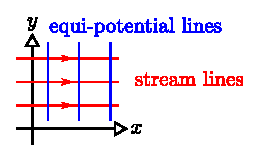
\includegraphics[scale=1.8]{figure/chapter5/5-1-1.eps}
%\caption{\label{fig:blue_rectangle} Rectangle}
\end{figure}
or
\begin{equation}
F(z) = Ve^{-i\alpha} z
\label{eq: 5-2-4}
\end{equation}
\begin{align*}
W(z) = \frac{dF}{dz}
&= Ve^{-i\alpha} \\
&= V\cos\alpha\mathbf{e_x} - iV\sin\alpha \mathbf{e_y}
\end{align*}
\begin{figure}[H]
\centering
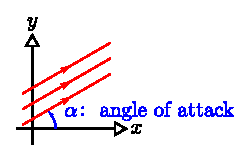
\includegraphics[scale=1.8]{figure/chapter5/5-1-2.eps}
%\caption{\label{fig:blue_rectangle} Rectangle}
\end{figure}
\item  Flow around a corner of arbitrary angle
\begin{equation}
F(z) = Az^n = A\left(re^{i\theta}\right)^n = Ar^ne^{in\theta}
\label{eq: 5-2-5}
\end{equation}
where $n$ is positive and $A$ is real number $>0$\\
i.e. 
\[
\left\{
\begin{aligned}
\Phi &= Ar^n\cos n\theta \\
\Psi &= Ar^n\sin n\theta
\end{aligned}
\right.
\]
and
\begin{subequations}
\begin{align}[left = \empheqlbrace\,]
v_r = \frac{\partial\Phi}{\partial r} &= nAr^{n-1}\cos n\theta \label{eq: 5-2-6a} \\
v_\theta = \frac{1}{r}\frac{\partial\Phi}{\partial \theta} &= -nAr^{n-1}\sin n\theta  \label{eq: 5-2-6b}
\end{align}
\end{subequations}
\begin{figure}[H]
\centering
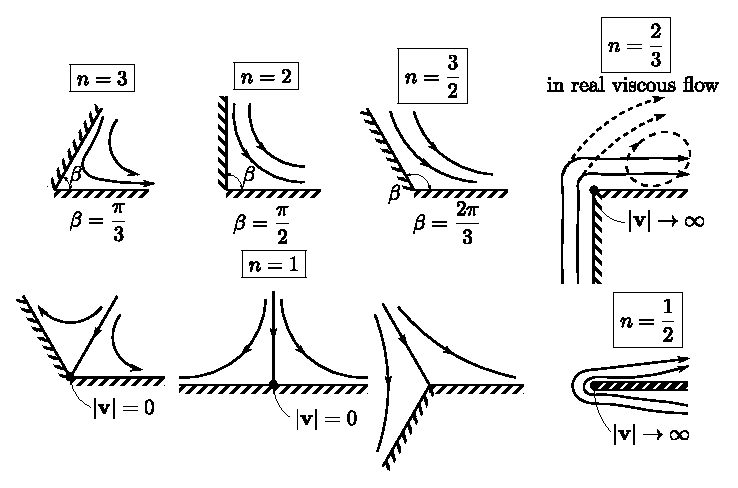
\includegraphics[scale=1.4]{figure/chapter5/5-1-3.eps}
%\caption{\label{fig:blue_rectangle} Rectangle}
\end{figure}
\[
\boxed{\beta = \frac{\pi}{n}}
\]
\item Plane (Line) Source/Sink
\begin{figure}[H]
\centering
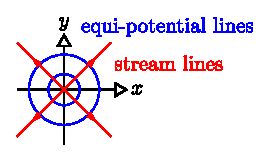
\includegraphics[scale=1.8]{figure/chapter5/5-1-4.eps}
%\caption{\label{fig:blue_rectangle} Rectangle}
\end{figure}
\begin{align}
F(z) &= m\ln z \label{eq: 5-2-7} \\
&=m\ln\left(re^{i\theta}\right) = m\ln r + im\theta\nonumber
\end{align}
where $m$ is real number, $m\colon +\longrightarrow$ source, $m\colon -\longrightarrow$ sink
\begin{subequations}
\begin{align}[left = \empheqlbrace\,]
\Phi &= m\ln r \label{eq: 5-2-8a}\\
\Psi &= m\theta \label{eq: 5-2-8b}
\end{align}
\end{subequations}
\begin{subequations}
\begin{align}[left = \empheqlbrace\,]
v_r &= \frac{m}{r} \label{eq: 5-2-9a}\\
v_\theta &= 0 \label{eq: 5-2-9b}
\end{align}
\end{subequations}
volume flow rate is
\[
Q = \oint_C\mathbf{v}\cdot\mathbf{n}dl = \int_0^{2\pi}v_rrd\theta = \int_0^{2\pi}\frac{m}{r}rd\theta = 2\pi m
\]
or 
\begin{equation}
F(z) = \frac{Q}{2\pi}\ln z
\label{eq: 5-2-10}
\end{equation}
If the origin of the source/sink is at $z_0$
\begin{equation}
F(z) = m\ln\left(z-z_0\right) = \frac{Q}{2\pi}\ln \left(z-z_0\right)
\label{eq: 5-2-11}
\end{equation}
\item Plane (Line) Vortex
\begin{figure}[H]
\centering
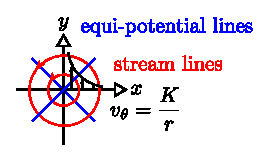
\includegraphics[scale=1.8]{figure/chapter5/5-1-5.eps}
%\caption{\label{fig:blue_rectangle} Rectangle}
\end{figure}
\begin{align}
F(z) &= -iK\ln z \label{eq: 5-2-12} \\
&=K\theta - iK\ln r\nonumber
\end{align}
where $K$ is real number.
\begin{subequations}
\begin{align}[left = \empheqlbrace\,]
\Phi &= K\theta \label{eq: 5-2-13a}\\
\Psi &= -K\ln r \label{eq: 5-2-13b}
\end{align}
\end{subequations}
\begin{subequations}
\begin{align}[left = \empheqlbrace\,]
v_r &= 0 \label{eq: 5-2-14a}\\
v_\theta &= \frac{K}{r} \label{eq: 5-2-14b}
\end{align}
\end{subequations}
Circulation is
\[
\Gamma = \oint_C\mathbf{v}\cdot\mathbf{t}dl = \int_0^{2\pi}v_\theta rd\theta = 2\pi K \neq 0
\]
or 
\begin{equation}
F(z) = -i\frac{\Gamma}{2\pi}\ln z
\label{eq: 5-2-15}
\end{equation}
If the origin of the vortex is at $z_0$
\begin{equation}
F(z) = -iK\ln\left(z-z_0\right) = -i\frac{\Gamma}{2\pi}\ln \left(z-z_0\right)
\label{eq: 5-2-16}
\end{equation}
\vspace{15em}
\item Plane (Line) Doublet (Dipole)
\vspace{5em}
\begin{figure}[H]
\centering
\begin{tikzpicture}[scale=2,transform canvas]
\draw [arrows = {-Latex[color=black, fill=white, length=3mm]}] (-2,0) -- (2,0) node [at end, above left] {$x$};
\draw [arrows = {-Latex[color=black, fill=white, length=3mm]}] (0,-2) -- (0,2) node [at end, left] {$y$};
\coordinate (P1) at (1,0);
\fill[color=black] (P1) circle[radius=2pt] node [below]{$m$(source)};
\coordinate (P2) at (-1,0);
\fill[color=black] (P2) circle[radius=2pt] node [below]{$-m$(sink)};
\draw[<->] (0,0.2) -- ($(P1)+(0,0.2)$) node [pos = 0.5, anchor=south]{$\epsilon$};
\draw[<->] (0,0.2) -- ($(P2)+(0,0.2)$) node [pos = 0.5, anchor=south]{$\epsilon$};
\end{tikzpicture}
\end{figure}
\vspace{5em}

\begin{align*}
F(z)
&= m\ln \left(z+\epsilon\right) - m\ln\left(z-\epsilon\right) \\
&= m\ln \frac{1+\epsilon/z}{1-\epsilon/z} \\
&= m\ln\left[1+2\frac{\epsilon}{z} + \mathcal{O}\left(\frac{\epsilon}{z}\right)^2\right] \\
&\cong m\left(2\frac{\epsilon}{z}\right)
\end{align*}
Let $\displaystyle\lim_{\epsilon\to 0}\left(2\epsilon m\right) = \mu$ where $\mu$ is real number
\begin{align}
\therefore 
F(z) &= \frac{\mu}{z} \label{eq: 5-2-17} \\
&= \frac{\mu}{re^{i\theta}} = \frac{\mu}{r}\cos\theta - i\frac{\mu}{r}\sin\theta \nonumber
\end{align}
\begin{subequations}
\begin{align}[left = \empheqlbrace\,]
\Phi &= \frac{\mu}{r}\cos\theta \label{eq: 5-2-18a}\\
\Psi &= -\frac{\mu}{r}\sin\theta \label{eq: 5-2-18b}
\end{align}
\end{subequations}
\begin{subequations}
\begin{align}[left = \empheqlbrace\,]
v_r &= -\frac{\mu}{r^2}\cos\theta \label{eq: 5-2-19a}\\
v_\theta &= -\frac{\mu}{r^2}\sin\theta \label{eq: 5-2-19b}
\end{align}
\end{subequations}
If origin of doublet is at $z-z_0$, then
\begin{equation}
F(z) = \frac{\mu}{z-z_0}
\label{eq: 5-2-20}
\end{equation}
\begin{figure}[H]
\centering
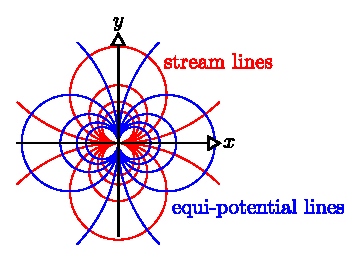
\includegraphics[scale=1.8]{figure/chapter5/5-1-6.eps}
%\caption{\label{fig:blue_rectangle} Rectangle}
\end{figure}
\begin{note}\mbox{}\\
\begin{enumerate}[label = \protect\circled{\arabic*}]
\item $\displaystyle\frac{d}{dz}\underbrace{\left(m\ln z\right)}_{=\text{source/sink}} = \underbrace{\frac{m}{z}}_{=\text{doublet}}$
\item $\displaystyle\frac{d}{dz}\underbrace{\left(\frac{m}{z}\right)}_{=\text{doublet}} = \underbrace{-\frac{m}{z^2}}_{=\text{quadruplet}}$
\begin{figure}[H]
\centering
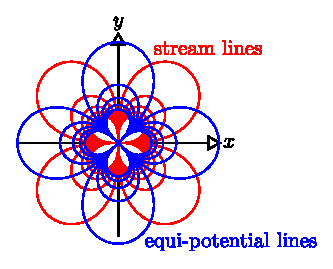
\includegraphics[scale=1.8]{figure/chapter5/5-1-7.eps}
%\caption{\label{fig:blue_rectangle} Rectangle}
\end{figure}
\item $\displaystyle\frac{1}{z^2},\frac{1}{z^3},\frac{1}{z^4},\cdots\colon$higher-order singularities
\end{enumerate}
\end{note}
\end{itemize}
\subsection{Images-Superposition}
\begin{itemize}
\item A singularities (source/sink, vortex, doublet, etc...) near an infinite plane wall
\begin{itemize}
\item source/sink
\begin{align*}
F(z) 
&= m\ln\left(z-ia\right) + m\ln\left(z+ia\right) \\
&= m\ln\left(z^2+a^2\right)
\end{align*}
\begin{figure}[H]
\centering
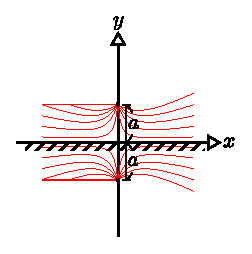
\includegraphics[scale=1.8]{figure/chapter5/5-1-8.eps}
%\caption{\label{fig:blue_rectangle} Rectangle}
\end{figure}
\item vortex
\begin{align*}
F(z) 
&= -\frac{i\Gamma}{2\pi}\ln\left(z-ia\right) + \frac{i\Gamma}{2\pi}\ln\left(z+ia\right) \\
&= \frac{i\Gamma}{2\pi}\ln\left(\frac{z+ia}{z-ia}\right)
\end{align*}
\begin{figure}[H]
\centering
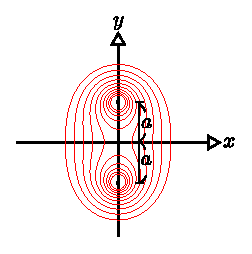
\includegraphics[scale=1.8]{figure/chapter5/5-1-9.eps}
%\caption{\label{fig:blue_rectangle} Rectangle}
\end{figure}
\end{itemize}
\item A singularity confined between two infinite plane walls\\
An infinite row of images of source 
\[
F(z) = m\sum_{n=-\infty}^{\infty}\ln\left(z+i2na\right)
\]
\begin{figure}[H]
\centering
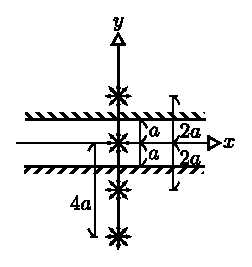
\includegraphics[scale=1.8]{figure/chapter5/5-1-10.eps}
%\caption{\label{fig:blue_rectangle} Rectangle}
\end{figure}
\item Distortion due to image
\begin{figure}[H]
\centering
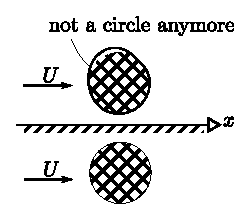
\includegraphics[scale=1.8]{figure/chapter5/5-1-11.eps}
%\caption{\label{fig:blue_rectangle} Rectangle}
\end{figure}
ref: A. B. Basset. On the motion of two spheres in a liquid, and allied problems. Proceedings of the London Mathematical Society
\end{itemize}
\subsection{Superposition-Flow around a circular cylinder with/without circulation}
\begin{itemize}
\item without circulation\\
Uniform stream + doublet: 
\[
F(z) = Uz + \frac{\mu}{z}
\]
require $r=a$ a streamline, then 
\[
F(ae^{i\theta}) = \left(Ua+ \frac{\mu}{a}\right)\cos\theta + i\left(Ua- \frac{\mu}{a}\right)\sin\theta
\]
\[
\Psi = \left(Ua - \frac{\mu}{a}\right)\sin\theta\Longrightarrow\Psi = 0\Longrightarrow\mu = Ua^2
\]
thus
\begin{equation}
F(z) = U\left(z + \frac{a^2}{z}\right)
\label{eq: 5-2-21}
\end{equation}
\begin{figure}[H]
\centering
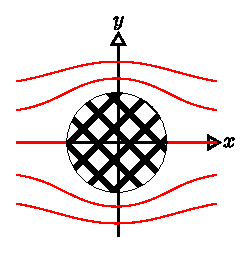
\includegraphics[scale=1.8]{figure/chapter5/5-1-12.eps}
%\caption{\label{fig:blue_rectangle} Rectangle}
\end{figure}
\item with circulation $\Gamma$\\
Can add a CW free vortex of strength $\Gamma$ to the above $F(z)$, i.e. uniform flow + doublet + vortex: 
\[
F(z) = U\left(z + \frac{a^2}{z}\right) + \frac{i\Gamma}{2\pi}\ln z + C
\]
require $r=a$ a streamline, then 
\begin{align*}
F(ae^{i\theta}) 
&= U\left(ae^{i\theta} + ae^{-i\theta}\right) + \frac{i\Gamma}{2\pi}\ln\left(ae^{i\theta}\right) + C \\
&= 2Ua\cos\theta - \frac{\Gamma\theta}{2\pi} + \frac{i\Gamma}{2\pi}\ln a + C
\end{align*}
choose $\displaystyle C = -\frac{i\Gamma}{2\pi}\ln a$, i.e. 
\begin{equation}
F(z) = U\left(z + \frac{a^2}{z}\right) + \frac{i\Gamma}{2\pi}\ln\frac{z}{a}
\label{eq: 5-2-22}
\end{equation}
\begin{subequations}
\begin{align}[left = \empheqlbrace\,]
\Phi &= U\cos\theta\left(r-\frac{a^2}{r}\right) - \frac{\Gamma\theta}{2\pi} \label{eq: 5-2-23a}\\
\Psi &= U\sin\theta\left(r-\frac{a^2}{r}\right) + \frac{\Gamma}{2\pi}\ln\frac{r}{a} \label{eq: 5-2-23b}
\end{align}
\end{subequations}
\begin{subequations}
\begin{align}[left = \empheqlbrace\,]
v_r &= U\cos\theta\left(1 - \frac{a^2}{r^2}\right) \label{eq: 5-2-24a}\\
v_\theta &= -U\sin\theta\left(1 + \frac{a^2}{r^2}\right) - \frac{\Gamma}{2\pi r} \label{eq: 5-2-24b}
\end{align}
\end{subequations}
On the surface of the circular cylinder  ($r=a$)
\[
\Longrightarrow
\left\{
\begin{aligned}
v_r &= 0 \\
v_\theta &= -2U\sin\theta - \frac{\Gamma}{2\pi a}
\end{aligned}
\right.
\]
Stagnation points
\begin{equation}
\Longrightarrow
\left\{
\begin{aligned}
v_r &= 0 \\
v_\theta &= 0
\end{aligned}
\right.
\Longrightarrow\sin\theta_s = -\frac{\Gamma}{4\pi Ua}
\label{eq: 5-2-25}
\end{equation}
\begin{figure}[H]
\centering
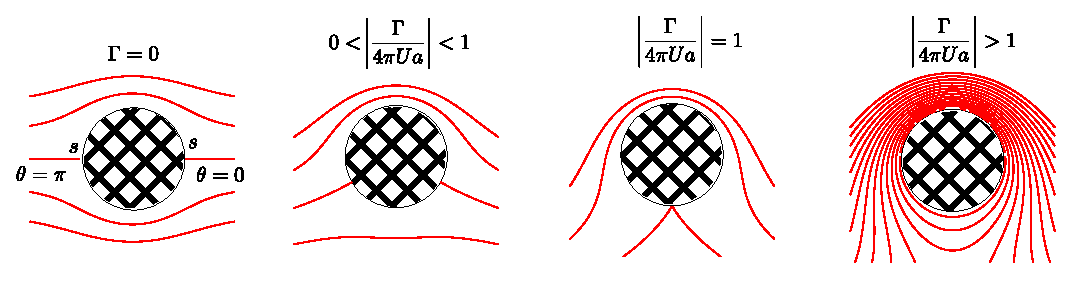
\includegraphics[scale=1.0]{figure/chapter5/5-1-13.eps}
%\caption{\label{fig:blue_rectangle} Rectangle}
\end{figure}
\end{itemize}
\subsection{The Circle Theorem (First)}
\begin{itemize}
\item Let $F(z)$ be the complex potential of a potential flow in the absence of any rigid boundaries and let all singularities of $F(z)$ be outside the circle $\abs{z} = a$.\\
If a circular cylinder $\abs{z} = a$ is introduced into the base flow $F(z)$, then the resulting complex potential $f(z)$ is given by 
\begin{equation}
f(z) = F(z) + \overline{F}(\frac{a^2}{z})\text{ (circle theorem)}
\label{eq: 5-2-26}
\end{equation}
\begin{proof}\mbox{}\\
\begin{enumerate}[label = \protect\circled{\arabic*}]
\item All singularities in $F(z)$ will lie inside the circle $\abs{z} = a$ in $\displaystyle\overline{F}(\frac{a^2}{z})$
\item If $z$ is on the circle $\abs{z} = a$, then $a^2/z = \bar{z}$, then 
\[
f(z) = F(z) + \overline{F}(\bar{z}) = \text{ real function}
\]
$\Longrightarrow\Psi = 0$ on $\abs{z} = a$, i.e. $\abs{z} =a$ is a streamline.
\end{enumerate}
\end{proof}
\begin{example}\mbox{}\\
\begin{figure}[H]
\centering
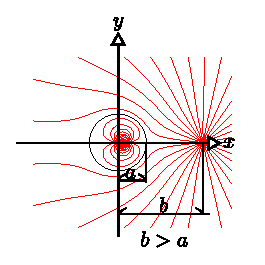
\includegraphics[scale=1.8]{figure/chapter5/5-1-14.eps}
%\caption{\label{fig:blue_rectangle} Rectangle}
\end{figure}
\[
F(z) = m\ln (z-b)
\]
\[
\Longrightarrow f(z) = m\ln\left(z-b\right) + m\ln\left(\frac{a^2}{z} - b\right)
\]
\end{example}
\end{itemize}
\subsection{Uniform Flow Past a Cylinder of Arbitrary Cross-Section}
\begin{itemize}
\item In general
\begin{align}
u - iv \equiv W(z) 
&\equiv\frac{dF(z)}{dz} = A_0 + \frac{A_1}{z} + \frac{A_2}{z^2} + \cdots\text{ (Laurent Series)}\nonumber \\
&= \sum_{n=0}^{\infty}\frac{A_n}{z_n}
\label{eq: 5-2-31}
\end{align}
\begin{equation}
\Longrightarrow
F(z) = \underbrace{A_0z}_{
\begin{subarray}{c}
  \text{uniform}\\
  \text{stream}
\end{subarray}
} + \underbrace{A_1\ln z}_{
\begin{subarray}{c}
  \text{source/sink}\\
  \text{or} \\
  \text{vortex}
\end{subarray}
} - \sum_{n=2}^\infty\frac{A_n}{n-1}\frac{1}{z^{n+1}} + \cancelto{0}{C}
\label{eq: 5-2-32}
\end{equation}
An $n\geq 2$ determined by geometry
\item About $A_0$ and $A_1$ in \eqref{eq: 5-2-32}\\
\begin{figure}[H]
\centering
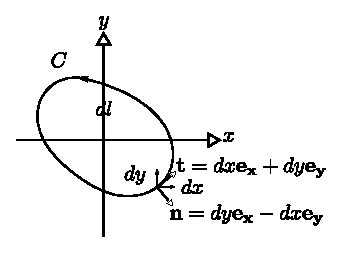
\includegraphics[scale=1.8]{figure/chapter5/5-1-15.eps}
%\caption{\label{fig:blue_rectangle} Rectangle}
\end{figure}
Note that 
\[
\Gamma = \ointctrclockwise_C\mathbf{v}\cdot\mathbf{t}dl = \ointctrclockwise_C\left(udx+vdy\right) = \ointctrclockwise_C d\Phi
\]
\[
Q = \ointctrclockwise_C\mathbf{v}\cdot\mathbf{n}dl = \ointctrclockwise_C\left(udy-vdx\right) = \ointctrclockwise_C d\Psi
\]
Hence 
\begin{align}
\Gamma + iQ
&= \ointctrclockwise_C\left(d\Phi + id\Psi\right)\nonumber \\
&= \ointctrclockwise_CdF = \ointctrclockwise_CW(z)dz\label{eq: 5-2-33}
\end{align}
In our present case, uniform free stream $U$ at $z\to\infty$. Hence $A_0 = U$ and
\begin{align*}
\Gamma + iQ
&= \ointctrclockwise_C W(z)dz \\
&= 0\text{ if $C$ does not enclose the cylinder}\\
&=2\pi iA_1\text{ for all circuits enclosing the cylinder}
\end{align*}
Let $A_1 = a_1 + ib_1$
\[
\Longrightarrow
\left\{
\begin{aligned}
\Gamma &= -2\pi b_1\Longrightarrow b_1 = -\frac{\Gamma}{2b} \\
Q &= 0 = 2\pi ia_1\Longrightarrow a_1 = 0
\end{aligned}
\right.
\]
for cylinder
\begin{equation}
W(z) = U - \frac{i\Gamma}{2\pi z} + \sum_{n=2}^\infty\frac{A_n}{z_n}
\label{eq: 5-2-34}
\end{equation}
\begin{equation}
F(z) = Uz - \frac{i\Gamma}{2\pi}\ln z + \sum_{n=2}^\infty\frac{A_n}{n-1}\frac{1}{z^{n-1}} + \cancelto{0}{C}
\label{eq: 5-2-35}
\end{equation}
\end{itemize}
\subsection{Force and Moment on a Cylinder}
\begin{itemize}
\item Blasius Theorem
\begin{figure}[H]
\centering
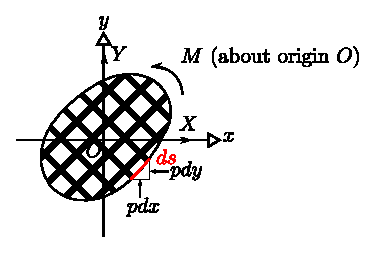
\includegraphics[scale=1.8]{figure/chapter5/5-1-16.eps}
%\caption{\label{fig:blue_rectangle} Rectangle}
\end{figure}
\begin{align*}
dX = -pdy, && dY = pdx, && dM = p\left(xdx + ydy\right)
\end{align*}
pressure: $p = p_\infty - \frac{\rho}{2}\abs{\mathbf{v}}^2$ can set $p_\infty = 0 $ without loss of generality.\\
Thus
\begin{align*}
d\left(X-iY\right) = \frac{\rho}{2}\abs{\mathbf{v}}^2\left(dy+idx\right), && dM = -\frac{\rho}{2}\abs{\mathbf{v}}^2\left(xdx + ydy\right)
\end{align*}
Now 
\begin{align*}
dy + idx = id\bar{z}, && xdx + ydy = \Re\left\{zd\bar{z}\right\}
\end{align*}
and 
\[
\abs{\mathbf{v}}^2 = W\overline{W} = \frac{dF}{dz}\frac{d\overline{F}}{d\bar{z}}
\]
Thus
\begin{align*}
d\left(X-iY\right) = \frac{\rho}{2}i\frac{dF}{dz}d\overline{F}, && dM = \Re\left\{-\frac{\rho}{2}z\frac{dF}{dz}d\overline{F}\right\}\text{ along $C$}
\end{align*}
On the cylinder, $\Psi = $ constant, $d\Psi = 0$\\
therefore
\[
d\overline{F} = d\left(\Phi - i\Psi\right) = d\left(\Phi + i\Psi\right) = dF = \frac{dF}{dz}dz
\]
along the cylinder surface\\
hence
\begin{align*}
d\left(X-iY\right) = \frac{\rho}{2}i\left(\frac{dF}{dz}\right)^2dz, && dM = \Re\left\{-\frac{\rho}{2}z\left(\frac{dF}{dz}\right)^2dz\right\}\text{ along $C$}
\end{align*}
i.e.
\begin{subequations}
\begin{align}[left = \empheqlbrace\,]
X - iY &= \frac{i\rho }{2}\oint_C\left(\frac{dF}{dz}\right)^2dz \label{eq: 5-2-40a} \\
M &= \Re\left\{-\frac{\rho}{2}\oint_Cz\left(\frac{dF}{dz}\right)^2dz\right\}  \label{eq: 5-2-40b}
\end{align}
\end{subequations}
$C$ could be any closed curve enclosing the cylinder
\end{itemize}
\subsection{Kutta-Joukowski Theorem}
\begin{figure}[H]
\centering
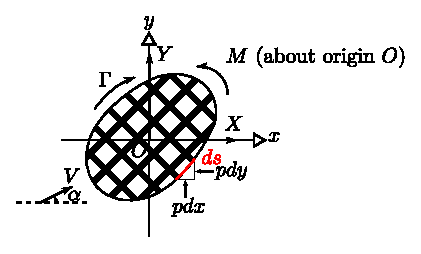
\includegraphics[scale=1.8]{figure/chapter5/5-1-17.eps}
%\caption{\label{fig:blue_rectangle} Rectangle}
\end{figure}
\begin{itemize}
\item Consider a cylinder (of arbitrary cross-section) placed in a uniform stream of speed $V$ at an angle-of-attack $\alpha$ with CW circulation of strength $\Gamma$. 
\begin{equation}
F(z) = Ve^{-i\alpha}z + \frac{i\Gamma}{2\pi}\ln z - \sum_{n=2}^{\infty}\frac{A_n}{n-1}\frac{1}{z^{n-1}}
\label{eq: 5-2-42}
\end{equation}
\[
\Longrightarrow W(z) = \frac{dF}{dz} = Ve^{-i\alpha} + \frac{i\Gamma}{2\pi z} + \sum_{n=2}^{\infty}\frac{A_n}{z^n}
\]
\[
\therefore W^2 = \underbrace{V^2e^{-2i\alpha}}_{B_0} + \underbrace{\frac{i\Gamma Ve^{-i\alpha}}{\pi}}_{B_{-1}}\frac{1}{z} + \underbrace{\frac{-\Gamma^2 + 8\pi^2A_2Ve^{-i\alpha}}{4\pi^2}}_{B_{-2}}\frac{1}{z^2} + \cdots
\]
From Blasius Theorem
\begin{align}
X - iY
&= \frac{i\rho}{2}\oint_CW^2(z)dz = \frac{i\rho}{2}2\pi i \left[B_{-1}\right]\nonumber \\
&= \frac{i\rho}{2}2\pi i\left(\frac{i\Gamma Ve^{-i\alpha}}{\pi}\right)\nonumber \\
&= -i\rho V e^{-i\alpha}\Gamma
\label{eq: 5-2-44}
\end{align}
or 
\begin{equation}
X + iY = \overline{X-iY} = i\rho V e^{-i\alpha}\Gamma
\label{eq: 5-2-45}
\end{equation}
In Aerodynamic:
\begin{align*}
\text{Lift force } L &\text{ is }\perp\text{ to free stream} \\
\text{Drag force } L &\text{ is }\parallel\text{ to free stream}
\end{align*}
\begin{equation}
D + iL = \left(X+iY\right)e^{-i\alpha} = i\rho V\Gamma
\label{eq: 5-2-46}
\end{equation}
\begin{subequations}
\begin{align}[left = \empheqlbrace\,]
L &= \rho V \Gamma\text{ (Kutta-Joukowski Theorem)} \label{eq: 5-2-47a} \\
D &= 0\text{ (d'Alembert paradox)}  \label{eq: 5-2-47b}
\end{align}
\end{subequations}
\item Moment on the cylinder 
\begin{align*}
M &= \Re\left\{-\frac{\rho}{2}\oint_CzW^2(z)dz\right\} = -\frac{\rho}{2}\Re\left\{2\pi i B_{-2}\right\} = \cdots \\ 
&= -2\pi \rho V\Re\left\{iA_2e^{-i\alpha}\right\}
\end{align*}

\end{itemize}
\section{Potential Flows Generated by Transformations}
\subsection{Conformal Transform (Mapping)}
General Properties
\begin{itemize}
\item Transformation (mapping) by analytic functions
\begin{figure}[H]
\centering
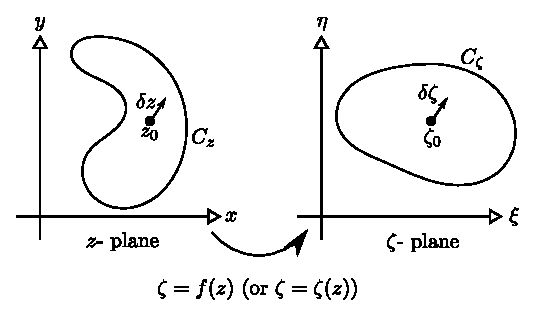
\includegraphics[scale=1.8]{figure/chapter5/5-1-18.eps}
%\caption{\label{fig:blue_rectangle} Rectangle}
\end{figure}
\begin{figure}[H]
\centering
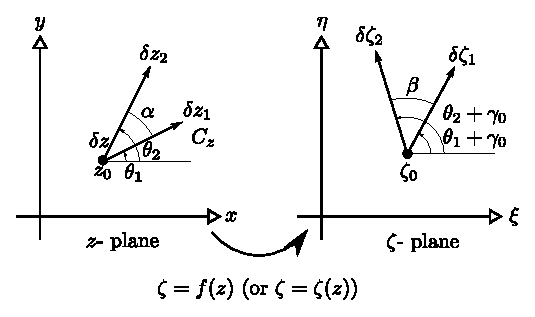
\includegraphics[scale=1.8]{figure/chapter5/5-1-19.eps}
%\caption{\label{fig:blue_rectangle} Rectangle}
\end{figure}
Assume $f(z)$ is analytic function and $\displaystyle\frac{d\zeta}{dz} = 0$, then 
\[
\delta\zeta = \left(\frac{d\zeta}{dz}\right)_{z_0}\delta z
\Longrightarrow\abs{\delta\zeta} = a_0\abs{\delta z},\arg(\delta\zeta) = \gamma_0+\arg(\delta z)\]
\[
\beta = \left(\theta_2+\gamma_0\right) - \left(\theta_1+\gamma_0\right) = \theta_2-\theta_1 = \alpha
\]
angle is preserved under mapping $\Longrightarrow$ Conformal mapping\\
What if $\boxed{\frac{d\zeta}{dz}=0} $ (critical point)
\item Analysis of the critical point of a transformation\\
Consider the transformation of form: 
\begin{align*}
\zeta = \left(z-z_0\right)^n \text{ ($n>1,n\colon$ integer)}, && \frac{d\zeta}{dz} = n\left(z-z_0\right)^{n-1}
\end{align*}
hence equal to zero at $z=z_0$
\begin{figure}[H]
\centering
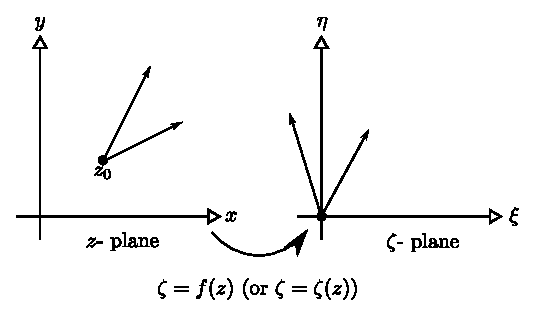
\includegraphics[scale=1.8]{figure/chapter5/5-1-20.eps}
%\caption{\label{fig:blue_rectangle} Rectangle}
\end{figure}
Let $z-z_0 = re^{i\theta}$, $\zeta = \rho e^{i\phi}$, then 
\begin{align*}
\zeta = \left(z-z_0\right)^n
&\Longrightarrow \rho e^{i\phi} = r^ne^{in\theta} \\
&\Longrightarrow \rho = r^n, \phi = n\theta\Longrightarrow\beta = n\alpha
\end{align*}
angle is not preserved at critical point under mapping.\\
Now consider the general transformation $\zeta = \zeta (z)$ and $z_0$ is a critical point
\[
\zeta(z) = \zeta(z_0) + a_1\left(z-z_0\right) + a_2\left(z-z_0\right)^2 + \cdots
\]
where
\[
a_k = \frac{1}{k!}\left(\frac{d^k\zeta}{dz^k}\right)_{z=z_0}
\]
Let us suppose the first $\left(n-1\right)$ derivatives are zero, i.e.
\[
a_1 = a_2 = a_3 = \cdots = a_{n-1} = 0,a_n\neq 0
\]
then
\[
\zeta = \zeta_0 + a_n\left(z - z_0\right)^n\overbrace{\left[1 + \frac{a_{n+1}}{a_n}\left(z-z_0\right) + \frac{a_{n+2}}{a_n}\left(z-z_0\right)^2 + \cdots\right]}^{f(z-z_0)}
\]
$\Longrightarrow \zeta-\zeta_0 = \left(z-z_0\right)^nf(z-z_0)$ as $z\to z_0$, $f(z-z_0)\approx 1 + O(z-z_0)$
\begin{example}\mbox{}\\
\begin{figure}[H]
\centering
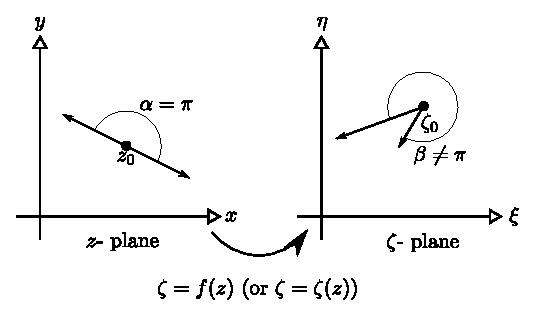
\includegraphics[scale=1.8]{figure/chapter5/5-1-21.eps}
%\caption{\label{fig:blue_rectangle} Rectangle}
\end{figure}
smooth curve will map to a sharp corner at critical point.
\end{example}
\item Application to the Potential Flow
\begin{enumerate}[label = (\alph*)]
\item \label{ch5-3-1-a} Consider a potential flow over certain configuration $C_z$ an $z$- plane with a complex potential $F(z)=\Phi(x,y) + i\Psi(x,y)$, suppose a conformal transformation $\zeta = \zeta(z)$, $\zeta = \xi + i\eta$, $z = x+iy$, which maps $C_z$ on $z$- plane into a relatively simple configuration $C_\zeta$ (e.g. a circle) on $\zeta$- plane.
\begin{figure}[H]
\centering
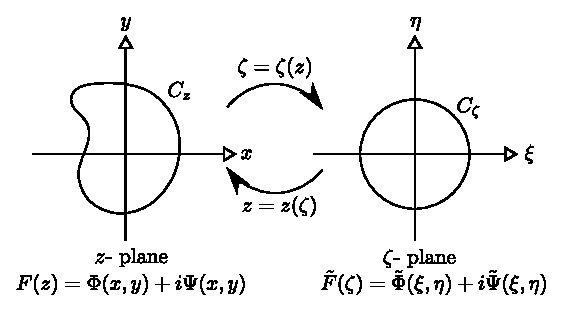
\includegraphics[scale=1.8]{figure/chapter5/5-1-22.eps}
%\caption{\label{fig:blue_rectangle} Rectangle}
\end{figure}
\begin{equation}
\tilde{F}(\zeta) = F(z(\zeta))
\label{eq: 5-3-1}
\end{equation}
Now
\[
\frac{d\tilde{F}}{d\zeta} = \frac{dF}{dz}\frac{dz}{d\zeta} = \frac{dF}{dz}/\frac{d\zeta}{dz}
\]
exists at all points where $d\zeta/dz\neq 0$\\
$\Longrightarrow\tilde{F}(\zeta)$ is an analytic function except at critical point of transformation.
\item The complex velocity on $\zeta$- plane
\begin{equation}
\tilde{W}(\zeta) = \frac{d\tilde{F}}{d\zeta} = \frac{dF}{dz}/\frac{d\zeta}{dz} = W(z)/\frac{d\zeta}{dz}
\label{eq: 5-3-2}
\end{equation}
$\tilde{W}(\zeta)\to\infty$ at the critical point $\displaystyle\frac{d\zeta}{dz} = 0$
\item Transformation of uniform condition at $\infty$
\begin{align*}
\frac{dz}{d\zeta}\to 1 &&\text{as}&&\zeta\to\infty
\end{align*}
i.e.
\begin{align*}
z\longleftrightarrow\zeta &&\text{as}&&\zeta\to\infty
\end{align*}
hence the form of the transformation
\[
z(\zeta) = \zeta + \frac{c_1}{\zeta} + \frac{c_2}{\zeta^2} + \cdots + = \zeta + \sum_{n=1}^\infty\frac{c_n}{\zeta^n}
\]
\item \label{ch5-3-1-d}
\begin{align*}
\Gamma_\zeta + iQ_\zeta
&= \oint_{C_\zeta}\overline{W}(\zeta)d\zeta = \oint_{C_\zeta}\frac{d\overline{F}}{d\zeta}d\zeta \\
&= \oint_{C_z}\frac{dF}{dz}\frac{dz}{d\zeta}d\zeta \\
&= \oint_{C_z}W(z)dz = \Gamma_z + iQ_z
\end{align*}
\end{enumerate}
Based on \ref{ch5-3-1-a}$\sim$\ref{ch5-3-1-d}
\begin{example}\mbox{}\\
Transformation of a uniform stream past a circular cylinder on $\zeta$- plane into that past an arbitrary cylinder on $z$- plane
\begin{equation}
z = \zeta + \frac{c_1}{\zeta} + \frac{c_2}{\zeta^2} + \cdots
\label{eq: 5-3-4}
\end{equation}
an from Blasius Theorem
\begin{equation}
\begin{aligned}
X - iY
&= \frac{i\rho}{2}\oint_{C_z}W^2(z)dz \\
&= \frac{i\rho}{2}\oint_{C_\zeta}W^2(\zeta)\left(\frac{d\zeta}{dz}\right)^2dz \\
&= \frac{i\rho}{2}\oint_{C_\zeta}W^2(\zeta)\frac{1}{dz/d\zeta}d\zeta
\end{aligned}
\label{eq: 5-3-5}
\end{equation}
\begin{equation}
\begin{aligned}
M
&= -\frac{\rho}{2}\Re\left\{\oint_{C_z}zW^2(z)dz\right\} \\
&= -\frac{\rho}{2}\Re\left\{\oint_{C_\zeta}z(\zeta)W^2(\zeta)\frac{1}{dz/d\zeta}d\zeta\right\}
\end{aligned}
\label{eq: 5-3-6}
\end{equation}
\end{example}
\end{itemize}
\subsection{Joukowski Transformation}
\begin{itemize}
\item General properties of J-T
\begin{equation}
z = \zeta + \frac{c^2}{\zeta}\text{ (J-T)}
\label{eq: 5-3-7}
\end{equation}
\begin{equation}
\frac{dz}{d\zeta} = 1 - \frac{c^2}{\zeta^2}
\label{eq: 5-3-8}
\end{equation}
As $\zeta\to \infty$, $\displaystyle\frac{dz}{d\zeta}\to 1$, i.e. $z\to\zeta$\\
A singular point at $\zeta = 0$; Two critical points at $\zeta = \pm c$
\begin{figure}[H]
\centering
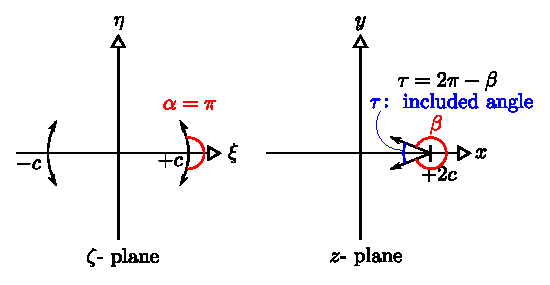
\includegraphics[scale=1.8]{figure/chapter5/5-1-23.eps}
%\caption{\label{fig:blue_rectangle} Rectangle}
\end{figure}
Previously, we have $\boxed{\beta = n\alpha}$\\
i.e. $2\pi-\tau = n\alpha\Longrightarrow \beta = n\alpha\Longrightarrow\tau = 2\pi -n\alpha$ where $n$ is the order of derivatives, i.e, $\displaystyle\frac{d^nz}{d\zeta^n}$ that first becomes non-zero.\\
\vspace{1em}
%----------------------
\begin{minipage}{0.4\textwidth}
For J-T, $n\equiv 2$, $\therefore\tau = 2\pi -n\alpha = 0$
\end{minipage} \hfill
\begin{minipage}{0.4\textwidth}
\begin{tikzpicture}[scale=2,transform canvas]
    \draw [color=black, -, rotate=0] ($(0,0.2)$) arc [start angle=210, end angle=270, x radius=1.2cm, y radius=0.6cm] node[above]{$\tau = 0$};
    \draw [color=black, -, rotate=0] ($(0,-0.4)$) arc [start angle=150, end angle=90, x radius=1.2cm, y radius=0.6cm] node[below]{\underline{cusp}};
\end{tikzpicture}
\end{minipage}\\
%----------------------
\end{itemize}
\subsection{Families of J-T}
\begin{enumerate}[label = (\alph*)]
\item Flow around elliptic cylinder \label{ch5-3-a}\\
Consider a circle of radius $a$ ($a>c$), centred at origin on $\zeta$- plane
\begin{figure}[H]
\centering
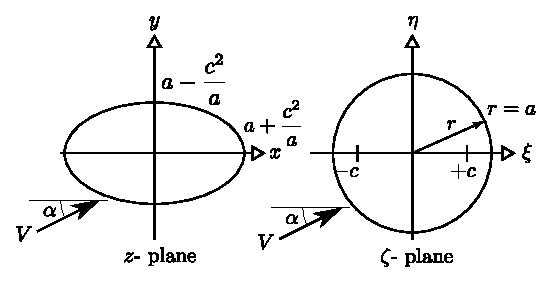
\includegraphics[scale=1.8]{figure/chapter5/5-1-24.eps}
%\caption{\label{fig:blue_rectangle} Rectangle}
\end{figure}
J-T
\begin{align*}
z = \zeta + \frac{c^2}{\zeta}, && \zeta = ae^{i\theta}
\end{align*}
\begin{align*}
\Longrightarrow
z 
&= ae^{i\theta} + \frac{c^2}{ae^{i\theta}} \\
&= \left(a + \frac{c^2}{a}\right)\cos\theta + i\left(a - \frac{c^2}{a}\right)\sin\theta \\
&= x + iy
\end{align*}
\[
\Longrightarrow
\left\{
\begin{aligned}
x &= \left(a + \frac{c^2}{a}\right)\cos\theta \\
y &= \left(a - \frac{c^2}{a}\right)\sin\theta
\end{aligned}
\right.
\]
or
\[
\left(\frac{x}{a+c^2/a}\right)^2 - \left(\frac{y}{a-c^2/a}\right)^2 = 1
\]
It is an ellipse!\\
Consider a uniform stream of speed $V$ and angle-of-attack $\alpha$ past the circular cylinder on $\zeta$- plane
\begin{equation}
F(\zeta) = V\left(e^{-i\alpha}\zeta + \frac{a^2}{\zeta}e^{i\alpha}\right)
\label{eq: 5-3-11}
\end{equation}
From J-T
\[
\zeta^2 - z\zeta + c^2 = 0\Longrightarrow\zeta \vc{=}{\footnotemark}{} \frac{z}{2}\pm\sqrt{\left(\frac{z}{2}\right)^2-c^2}
\]
\begin{align*}
\therefore F(z)
&= F(\zeta(z)) \\
&= V\left\{\left[\frac{z}{2} + \sqrt{\left(\frac{z}{2}\right)^2-c^2}\right]e^{-i\alpha} + \frac{a^2e^{i\alpha}}{\frac{z}{2} + \sqrt{\left(\frac{z}{2}\right)^2-c^2}}\right\} \\
&=V\left[ze^{-i\alpha} + \left(\frac{a^2}{c^2}e^{i\alpha} - e^{-i\alpha}\right)\left(\frac{z}{2}-\sqrt{\left(\frac{z}{2}\right)^2 - c^2}\right)\right]
\end{align*}
\footnotetext{discard $-$ since $z\to\zeta$ as $\zeta\to\infty$}
\begin{figure}[H]
\centering
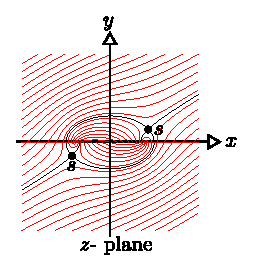
\includegraphics[scale=1.8]{figure/chapter5/5-1-25.eps}
%\caption{\label{fig:blue_rectangle} Rectangle}
\end{figure}
\begin{example}{Stagnation points on the ellipse}\mbox{}\\
$\zeta = \pm ae^{i\alpha}$ subs into J-T 
\begin{equation}
z = \zeta + \frac{c^2}{\zeta}\Longrightarrow z = \pm \left(a + \frac{c^2}{a}\right)\cos\alpha \pm i\left(a - \frac{c^2}{a}\right)\sin\alpha
\end{equation}
\end{example}
\item Flow around a flat plate \label{ch5-3-b}
\begin{figure}[H]
\centering
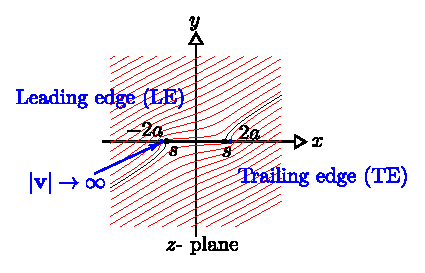
\includegraphics[scale=1.8]{figure/chapter5/5-1-26.eps}
%\caption{\label{fig:blue_rectangle} Rectangle}
\end{figure}
In \ref{ch5-3-a}, let $c=a$, the $\zeta = ae^{i\theta}\vc{\Longrightarrow}{\text{maps to}}{}-2a\leq x\leq 2a$ on $z$- plane
\begin{equation}
F(z) = V\left[ze^{-i\alpha} + \left(e^{i\alpha} - e^{-i\alpha}\right)\left(\frac{z}{2}-\sqrt{\left(\frac{z}{2}\right)^2-a^2}\right)\right]
\end{equation}
\begin{example}{Stagnation points on the plate}\mbox{}\\
$\zeta = \pm ae^{i\alpha}$ subs into J-T 
\begin{equation}
z = \zeta + \frac{c^2}{\zeta}\Longrightarrow z = \pm 2a\cos\alpha 
\end{equation}
\end{example}
\item Flow around a circular arc (camber line) \label{ch5-3-c}
\begin{figure}[H]
\centering
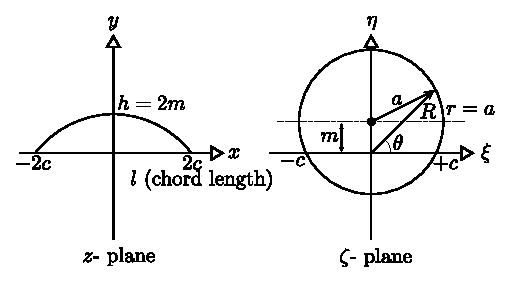
\includegraphics[scale=1.8]{figure/chapter5/5-1-27.eps}
%\caption{\label{fig:blue_rectangle} Rectangle}
\end{figure}
From $\zeta = R(\theta)e^{i\theta}$ and J-T: $\displaystyle z = Re^{i\theta} + \frac{c}{R^2}e^{-i\theta}$
\[
\Longrightarrow
\left\{
\begin{aligned}
x &= \left(R + \frac{c^2}{R}\right)\cos\theta \\
y &= \left(R - \frac{c^2}{R}\right)\sin\theta
\end{aligned}
\right.
\]
\begin{equation}
\vc{\Longrightarrow}{\text{eliminating}}{R}
x^2\sin^2\theta - y^2\cos^2\theta = 4c^2\sin^2\theta\cos^2\theta
\label{eq: 5-3-16}
\end{equation}
use relation
\begin{equation}
c^2+m^2 = a^2 = R^2 + m^2 - 2Rm\overbrace{\cos\left(\frac{\pi}{2}-\theta\right)}^{\sin\theta}
\tag{$\ast$}
\label{eq: 5-3-*}
\end{equation}
\begin{example}\mbox{}\\
\begin{equation}
\eqref{eq: 5-3-16}\Longrightarrow
x^2 + \left[y+c\left(\frac{c}{m}-\frac{m}{c}\right)\right]^2 = c^2\left[4+\left(\frac{c}{m}-\frac{m}{c}\right)^2\right]
\label{eq: 5-3-17}
\end{equation}
\begin{solution}\mbox{}\\
From \eqref{eq: 5-3-*}
\[
\sin\theta = \frac{R^2-c^2}{2Rm}\text{ and } \sin\theta= \frac{y}{R-c^2/R}\Longrightarrow\sin\theta = \frac{y}{2m\sin\theta}
\]
\begin{align*}
\Longrightarrow\sin^2\theta = \frac{y}{2m}, &&\cos^2\theta = 1-\sin^2\theta = 1-\frac{y}{2m}
\end{align*}
\end{solution}
\end{example}
\[
\eqref{eq: 5-3-17}\Longrightarrow
\left\{
\begin{aligned}
l &= 4c \\
h &= 2m
\end{aligned}
\right.
\Longrightarrow
\left\{
\begin{aligned}
c &= \frac{l}{4} \\
m &= \frac{h}{2}
\end{aligned}
\right.
\text{ If we let }\frac{m}{c} = \epsilon\ll 1
\]
then
\begin{subequations}
\begin{equation}
x^2 + \left(y+\frac{c^2}{m}\right)^2 = c^2\left(4+\frac{c^2}{m^2}\right) + \mathcal{O}(\epsilon^2)
\label{eq: 5-3-18a}
\end{equation}
correct to $\mathcal{O}(\epsilon)$\\
in terms of $l$ and $h$
\begin{equation}
x^2 + \left(y+\frac{l^2}{8h}\right)^2 = \frac{l^2}{4}\left(1+\frac{l^2}{16h^2}\right)
\label{eq: 5-3-18b}
\end{equation}
\end{subequations}
The complex potential is
\begin{equation}
F(\zeta) = V\left[\left(\zeta-im\right)e^{-i\alpha}+\frac{a^2}{\zeta-im}e^{i\alpha}\right]
\label{eq: 5-3-19}
\end{equation}
with
\[
z = \zeta + \frac{c^2}{\zeta}
\]
\begin{figure}[H]
\centering
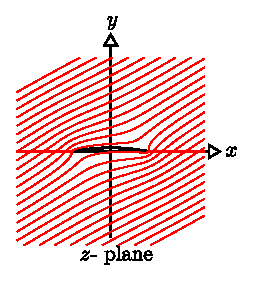
\includegraphics[scale=1.8]{figure/chapter5/5-1-28.eps}
%\caption{\label{fig:blue_rectangle} Rectangle}
\end{figure}
\item Flow around a symmetric Joukowski airfoil  \label{ch5-3-d}
\begin{figure}[H]
\centering
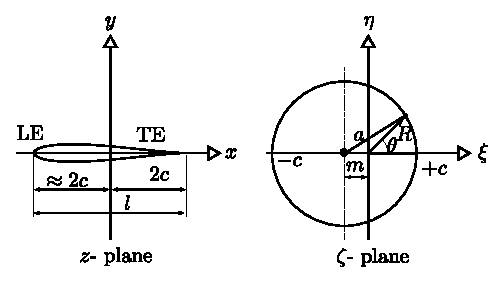
\includegraphics[scale=1.8]{figure/chapter5/5-1-29.eps}
%\caption{\label{fig:blue_rectangle} Rectangle}
\end{figure}
From J-T and infinitesimal assumption
\begin{align*}
z = \zeta + \frac{c^2}{\zeta}, && \epsilon = \frac{m}{c}\ll 1
\end{align*}
hence $\zeta = c\Longrightarrow z = 2c$
\[
\zeta = -\left(c+2m\right)\Longrightarrow z = -c\left(1+2\epsilon\right)-\frac{c}{1+2\epsilon} = -2c + \mathcal{O}(\epsilon^2)
\]
hence
\[
l\approx 4c + \mathcal{\epsilon^2}
\]
\begin{exercise}{Show that correct to $\mathcal{\epsilon}$, the airfoil shape on $z$- plane is given by}
\[
z\approx c\left[2\cos\theta+i2\epsilon\left(1-\cos\theta\right)\sin\theta\right] + \mathcal{O}(\epsilon^2)
\]
i.e.
\[
\left\{
\begin{aligned}
x &\approx 2c\cos\theta \\
y &\approx 2c\epsilon\left(1-\cos\theta\right)\sin\theta
\end{aligned}
\right.
\]
or
\begin{equation}
y \approx \pm 2c\epsilon\left(1-\frac{x}{2c}\right)\sqrt{1-\left(\frac{x}{2c}\right)^2} + \mathcal{O}(\epsilon^2)
\label{eq: 5-3-20}
\end{equation}
\begin{solution}\mbox{}\\
From cosine theorem
\begin{align*}
a^2 = \left(c+m\right)^2
&= R^2\left(1+\frac{m^2}{R^2} + 2\frac{m}{R}\cos\theta\right) \\
&\vc{=}{\footnotemark}{}R^2\left(1+2\underbrace{\frac{m}{R}}_{\mathcal{O}(\epsilon)}\cos\theta + \mathcal{O}(\epsilon^2)\right)
\end{align*}
\footnotetext{From $R\geq c$, $m/R\leq m/c$, i.e. $m/R=\mathcal{O}(\epsilon)$}
\[
\Longrightarrow c+m \approx R\left(1+\frac{m}{R}\cos\theta\right)
\]
\[
\therefore R\approx c\left[1+\epsilon\left(1-\cos\theta\right)\right]
\]
From J-T
\begin{align*}
z 
&= \zeta + \frac{c^2}{\zeta} \\
&= Re^{i\theta} + \frac{c^2}{R}e^{-i\theta} \\
&= c\left[1+\epsilon\left(1-\cos\theta\right)\right]e^{i\theta} + \frac{ce^{-i\theta}}{1+\epsilon\left(1-\cos\theta\right)} \\
&\vc{=}{\footnotemark}{}c\left[1+\epsilon\left(1-\cos\theta\right)\right]e^{i\theta} + c\left[1-\epsilon\left(1-\cos\theta\right)+\mathcal{O}(\epsilon^2)\right]e^{-i\theta}
\end{align*}
\footnotetext{$\displaystyle\frac{ce^{-i\theta}}{1+\epsilon\left(1-\cos\theta\right)} = ce^{-i\theta}\left[1-\epsilon\left(1-\cos\theta\right)+\mathcal{O}(\epsilon^2)\right]$}
\end{solution}
\end{exercise}
Maximum thickness $t$ occurs at $\displaystyle\frac{dy}{dx} = 0$
\[
\Longrightarrow
\left\{
\begin{aligned}
x & = -c \\
y & = \pm\frac{3\sqrt{3}}{2}c\epsilon
\end{aligned}
\right.
\Longrightarrow t\approx 3\sqrt{3}c\epsilon
\]
hence thickness ratio
\[
\frac{t}{l} = \frac{3\sqrt{3}}{4}\epsilon\Longrightarrow\epsilon = \frac{m}{c}\approx\frac{4}{3\sqrt{3}}\frac{t}{l} \approx 0.77\frac{t}{l}
\]
equation for the airfoil in terms of $t$ and $l$
\begin{equation}
\frac{y}{t}\approx\pm 0.385\left(1-2\frac{x}{l}\right)\sqrt{1-\left(\frac{2x}{l}\right)^2}
\label{eq: 5-3-21}
\end{equation}
The complex potential is
\begin{equation}
F(\zeta) = V\left[\left(\zeta+m\right)e^{-i\alpha} + \frac{a^2}{\zeta + m}e^{i\alpha}\right]
\label{eq: 5-3-22}
\end{equation}
\begin{figure}[H]
\centering
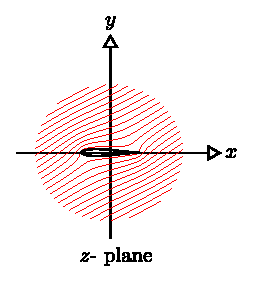
\includegraphics[scale=1.8]{figure/chapter5/5-1-30.eps}
%\caption{\label{fig:blue_rectangle} Rectangle}
\end{figure}
\item Flow around a cambered Joukowski airfoil\label{ch5-3-e}
\begin{figure}[H]
\centering
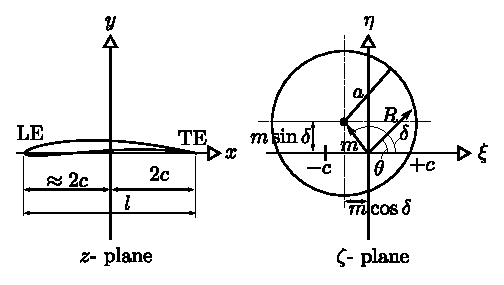
\includegraphics[scale=1.8]{figure/chapter5/5-1-31.eps}
%\caption{\label{fig:blue_rectangle} Rectangle}
\end{figure}
For $\epsilon = m/c\ll 1$\\
correct to $\mathcal{O}(\epsilon)$, equation of the cambered Joukowski airfoil
\begin{equation}
\begin{aligned}
y 
&= \underbrace{\sqrt{\frac{l^2}{4}\left(1+\frac{l^2}{16h^2}\right)-x^2}-\frac{l^2}{8h}}_{
\begin{subarray}{c}
  \text{equation for camber}\\
  \text{\eqref{eq: 5-3-18b}}
\end{subarray}
} \\
&\pm\underbrace{ 0.385\left(1-2\frac{x}{l}\right)\sqrt{1-\left(\frac{2x}{l}\right)^2} + \mathcal{O}(\frac{t}{l})^2}_{
\begin{subarray}{c}
  \text{equation for thickness}\\
  \text{\eqref{eq: 5-3-21}}
\end{subarray}
}
\end{aligned}
\label{eq: 5-3-23}
\end{equation}
The complex potential is
\begin{equation}
F(\zeta) = V\left[\left(\zeta - me^{i\delta}\right)e^{-i\alpha} + \frac{a^2e^{i\alpha}}{\zeta - me^{i\delta}}\right]
\label{eq: 5-3-24}
\end{equation}
with $\displaystyle z = \zeta + \frac{c^2}{\zeta}$ and
\begin{align*}
m\cos\delta\approx\frac{0.77}{4}t, && m\sin\delta\approx\frac{h}{2}, && a\approx\frac{l}{4}\left(1+0.77\frac{t}{l}\right)
\end{align*}
\end{enumerate}
\subsection{Kutta Condition}
Above \ref{ch5-3-b}$\sim$\ref{ch5-3-e} cases all involve a singular point at TE where velocity $\to\infty$. The viscous effect must take action.
\begin{itemize}
\item Kutta-Joukowski hypothesis\\
Whenever a flow passing around sharp corner, the viscous effect becomes significant and cannot be neglected therefore,\\
instead of 
\begin{figure}[H]
\centering
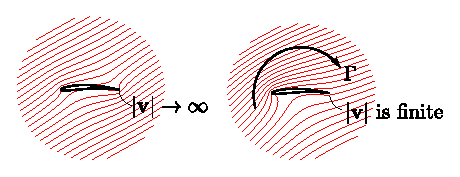
\includegraphics[scale=1.8]{figure/chapter5/5-1-32.eps}
%\caption{\label{fig:blue_rectangle} Rectangle}
\end{figure}
These should be a circulation around the airfoil as a manifestation of the viscous effect (flow separation), the magnitude of the circulation being such that to ensure the flow leave the TE smoothly, i.e.\\
$\Gamma$ is fixed by the requirement
\begin{equation}
\frac{dF(z)}{dz} = \frac{dF}{d\zeta}/\frac{dz}{d\zeta}\text{ is finite at TE}
\label{eq: 5-3-30}
\end{equation}
which implies
\begin{equation}
\frac{dF}{d\zeta} = 0\text{ at TE (at critical point $\zeta = c$)}
\label{eq: 5-3-31}
\end{equation}
\begin{figure}[H]
\centering
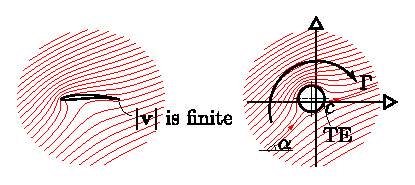
\includegraphics[scale=1.8]{figure/chapter5/5-1-33.eps}
%\caption{\label{fig:blue_rectangle} Rectangle}
\end{figure}
\item Generation of Stating Vortex and Bound Vortex \\
Consider
\begin{figure}[H]
\centering
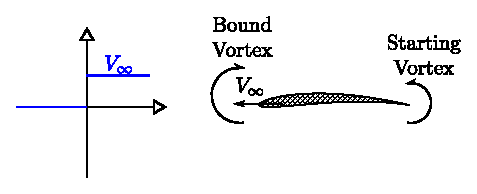
\includegraphics[scale=1.8]{figure/chapter5/5-1-34.eps}
%\caption{\label{fig:blue_rectangle} Rectangle}
\end{figure}
%----------------------
\begin{minipage}{0.1\textwidth}
\begin{figure}[H]
\centering
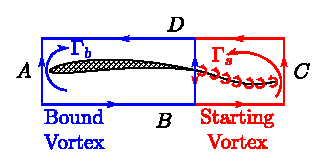
\includegraphics[scale=1.8]{figure/chapter5/5-1-35.eps}
%\caption{\label{fig:blue_rectangle} Rectangle}
\end{figure}
\end{minipage}\hfill
\begin{minipage}{0.35\textwidth}
From Kelvin's Theorem
\[
\frac{D\Gamma_{ABCD}}{Dt} = 0\Longrightarrow\Gamma_{ABCD} = 0
\]
\[
\Gamma_b-\Gamma_s = \Gamma_{ABCD} = 0
\]
\[
\Gamma_b = - \Gamma_s
\]
\end{minipage}\\
\vspace{2em}
%----------------------
\item Back to the Joukowski-airfoil problems
\begin{figure}[H]
\centering
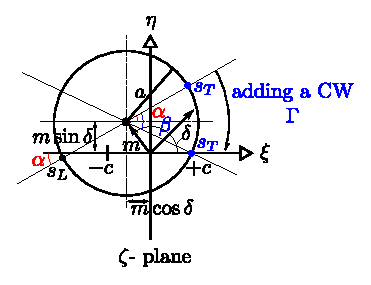
\includegraphics[scale=1.8]{figure/chapter5/5-1-36.eps}
%\caption{\label{fig:blue_rectangle} Rectangle}
\end{figure}
Recall 
\[
F(\zeta) = V\left[\left(\zeta-\zeta_0\right)e^{-i\alpha} + \frac{a^2e^{i\alpha}}{\zeta-\zeta_0}\right] + \frac{i\Gamma}{2\pi}\ln\left(\zeta-\zeta_0\right)
\]
\begin{equation}
W(\zeta) = \frac{dF}{d\zeta} = Ve^{-i\alpha} + \frac{i\Gamma}{2\pi}\frac{1}{\zeta - \zeta_0} - Ve^{i\alpha}a^2\frac{1}{\left(\zeta-\zeta_0\right)}
\label{eq: 5-3-32}
\end{equation}
From geometry: $c-\zeta_0 = ae^{-i\beta}$\\
at $TE$: $\zeta = c$
\[
W(c) = Ve^{-i\alpha} + \frac{i\Gamma}{2\pi}e^{i\beta} - Ve^{i\left(\alpha+2\beta\right)}
\]
KC require $W(c) = 0$
\[
\Longrightarrow 2\pi a V\left[1-e^{2i\left(\alpha+\beta\right)}\right] + i\Gamma e^{i\left(\alpha+\beta\right)} = 0
\]
\[
\Longrightarrow \Gamma = 4\pi a V\sin\left(\alpha+\beta\right)
\]
The lift on the Joukowski airfoil is
\begin{equation}
L = \rho V\Gamma = 4\pi a\rho V^2\sin\left(\alpha+\beta\right)
\label{eq: 5-3-33}
\end{equation}
the lift coefficient $C_L$ is defined as
\begin{equation}
C_L = \frac{L}{\frac{\rho}{2}V^2l} = 8\pi\left(\frac{a}{l}\right)\sin\left(\alpha+\beta\right)
\label{eq: 5-3-34}
\end{equation}
For small angle-of-attack, $\alpha\ll 1$, and small $\beta$ (which corresponds to \emph{thin} airfoil) $\beta\ll 1$,
\[
\sin\left(\alpha+\beta\right)\approx\alpha + \beta
\]
hence
\begin{equation}
L\approx 4\pi\rho V^2 a\left(\alpha+\beta\right)
\label{eq: 5-3-35}
\end{equation}
\begin{equation}
C_L\approx 8\pi\left(\frac{a}{l}\right)\left(\alpha+\beta\right)
\label{eq: 5-3-35}
\end{equation}
Furthermore, if $\beta \ll 1$, $l\approx 4c\approx 4a$, hence
\begin{equation}
L\approx \pi\rho lV^2\left(\alpha+\beta\right)
\label{eq: 5-3-36}
\end{equation}
\begin{equation}
\boxed{C_L\approx 2\pi\left(\alpha+\beta\right)}
\label{eq: 5-3-37}
\end{equation}
where $\alpha$ is angle-of-attack and $\beta$ is related to camber $\approx\displaystyle\frac{2h}{l}$
\begin{note}\mbox{}\\
\begin{enumerate}[label = \protect\circled{\arabic*}]
\item $L\neq 0$ at $\alpha = 0$ (due to camber) \\
\item $L = 0$ when $\alpha =-\beta$, $-\beta\equiv\alpha_0$, where $\alpha_0$ is zero-left angle \\
Define an effective angle-of-attack $\alpha_e$
\begin{align*}
\alpha_e = \alpha - \alpha_0 = \alpha + \beta, && C_L\approx 2\pi \alpha_e
\end{align*}
\end{enumerate}
\begin{figure}[H]
\centering
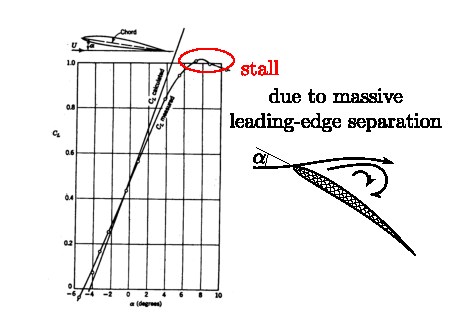
\includegraphics[scale=1.8]{figure/chapter5/5-1-37.eps}
%\caption{\label{fig:blue_rectangle} Rectangle}
\end{figure}
\end{note}
\end{itemize}
\begin{example}\mbox{}\\
\begin{figure}[H]
\centering
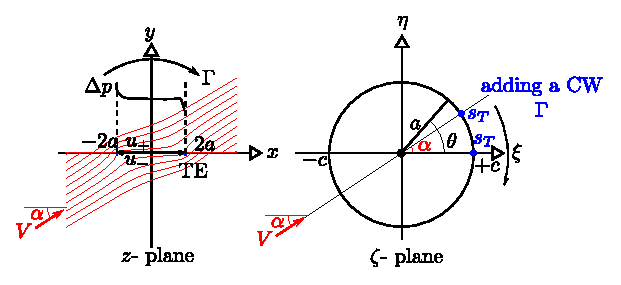
\includegraphics[scale=1.8]{figure/chapter5/5-1-38.eps}
%\caption{\label{fig:blue_rectangle} Rectangle}
\end{figure}
\[
F(\zeta) = V\left(\zeta e^{-i\alpha} + \frac{a^2}{\zeta}e^{i\alpha}\right) + \frac{i\Gamma}{2\pi}\ln\zeta
\]
\[
\frac{dF}{dz} = \frac{dF}{d\zeta}/\frac{dz}{d\zeta} \equiv\text{ finite at TE }(\zeta = a)
\]
i.e.
\begin{align*}
\left.\frac{dF}{d\zeta}\right|_{\zeta = a} = 0, &&\frac{dF}{d\zeta} = Ve^{-i\alpha} - V\frac{a^2e^{i\alpha}}{\zeta^2} + \frac{i\Gamma}{2\pi}\frac{1}{\zeta}
\end{align*}
\[
\left.\frac{dF}{d\zeta}\right|_{\zeta = a} = 0\Longrightarrow Ve^{-i\alpha} - Ve^{i\alpha} + \frac{i\Gamma}{2\pi a} = 0
\]
\[
\Longrightarrow\boxed{\Gamma = 4\pi Va\sin\alpha}
\]
Velocity on the plate:
\begin{align*}
\left.\frac{dF}{d\zeta}\right|_{\text{plate}} \equiv\left.\frac{dF}{d\zeta}\right|_{\zeta = ae^{i\theta}}
&= Ve^{-i\alpha} - Ve^{i\left(\alpha-2\theta\right)} + \frac{i\Gamma}{2\pi a}e^{-i\theta} = \cdots \\
&= Ve^{-i\theta}\left[e^{-i\left(\alpha-\theta\right)} - e^{i\left(\alpha-\theta\right)} + i2\sin\alpha\right] \\
&= 2iVe^{-i\theta}\left[\sin\alpha-\sin\left(\alpha-\theta\right)\right]
\end{align*}
\[
\left.\frac{dz}{d\zeta}\right|_{\text{plate}}\equiv\left.\frac{dz}{d\zeta}\right|_{\zeta = ae^{i\theta}} = 1-e^{-2i\theta} = e^{-i\theta}\left[e^{i\theta}-e^{-i\theta}\right] = 2i\sin\theta e^{-i\theta}
\]
\begin{align*}
\Longrightarrow
\left.\frac{dF}{dz}\right|_{\text{plate}} = \left.\frac{dF}{d\zeta}/\frac{dz}{d\zeta}\right|_{\text{plate}}
&= \frac{2iVe^{-i\theta}\left[\sin\alpha-\sin\left(\alpha-\theta\right)\right]}{2i\sin\theta e^{-i\theta}} \\
&= \frac{V\left[\sin\alpha-\sin\alpha\cos\theta+\cos\alpha\sin\theta\right]}{\sin\theta}\\ 
&= \cdots \\
&= V\cos\alpha\left(1+\tan\alpha\frac{1-\cos\theta}{\sin\theta}\right)\equiv \left.u-iv\right|_{\text{plate}}
\end{align*}
on the plate
\[
\left\{
\begin{aligned}
u &= V\cos\alpha\left(1+\tan\alpha\frac{1-\cos\theta}{\sin\theta}\right), 0<\theta\leq \pi\colon\text{upper surface of plate} \\
v &= 0,\pi<\theta\leq 2\pi\colon\text{lower surface of plate}
\end{aligned}
\right.
\]
From Bernoulli's equation
\[
p_+ + \frac{\rho}{2}u_+^2 = p_- + \frac{\rho}{2}u_-^2
\]
\begin{align*}
\Delta p
&\equiv p_- - p_+ = \frac{\rho}{2}\left(u_+^2 - u_-^2\right) \\
&= \frac{\rho}{2}V^2\cos^2\alpha\left[\left(1 + \tan\alpha\frac{1-\cos\theta}{\sin\theta}\right)^2 - \left(1 - \tan\alpha\frac{1-\cos\theta}{\sin\theta}\right)^2\right] \\
&= \rho V^2\sin\alpha\frac{1-\cos\theta}{\sin\theta}, \text{ $0\leq\theta\leq\pi$}
\end{align*}
Lift force $Y$
\begin{align*}
Y 
&= \int_{-2a}^{2a}\Delta p dx \vc{=}{\footnotemark}{} \int_{\theta = \pi}^{\theta = 0}\Delta p d\left(2a\cos\theta\right) = 2a\int_0^{\pi}\Delta p \sin\theta d\theta  \\
&= 2\rho V^2a\sin 2\alpha\int_0^{\pi}\left(1-\cos\theta\right)d\theta = 2\pi\rho V^2a\sin 2\alpha
\end{align*}
\footnotetext{From J-T $\displaystyle z = \zeta + \frac{a^2}{\zeta},\zeta = ae^{i\theta}$, $z=a^{i\theta} + ae^{-i\theta} = 2a\cos\theta = x+iy\Longrightarrow
\left\{
\begin{aligned}
x &= 2a\cos\theta \\
y &= 0
\end{aligned}
\right.
$}
or from Kutta-Joukowski Theorem
\begin{align*}
X - iY = -i\rho Ve^{-i\alpha}\Gamma, &&\text{ Here }\Gamma = 4\pi Va\sin\alpha
\end{align*}
\[
\therefore X-iY = -4\pi\rho V^2a\sin^2\alpha-i4\pi\rho V^2a\sin\alpha\cos\alpha
\]
\[
\Longrightarrow
\left\{
\begin{aligned}
X &= -4\pi\rho V^2a\sin^2\alpha\neq 0 \\
Y &= 4\pi \rho V^2a\sin\alpha\cos\alpha
\end{aligned}
\right.
\]
\end{example}
\subsection{Schwarz-Christoffel Transformation}
\begin{figure}[H]
\centering
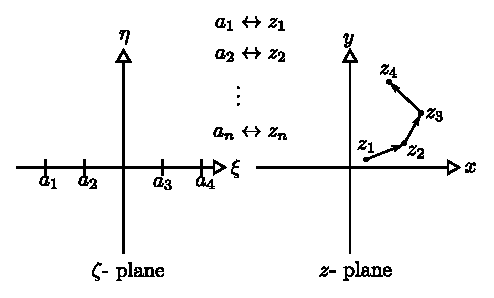
\includegraphics[scale=1.8]{figure/chapter5/5-1-39.eps}
%\caption{\label{fig:blue_rectangle} Rectangle}
\end{figure}
At critical point of transformation
\[
\text{A smooth curve}\Longleftrightarrow\text{A corner}
\]
The transformation has the form
\begin{equation}
\frac{dz}{d\zeta} = K\left(\zeta-a_1\right)^{k_1-1}\left(\zeta-a_2\right)^{k_2-1}\cdots\left(\zeta-a_N\right)^{k_N-1} \text{ (S-C T)}
\label{eq: 5-3-60}
\end{equation}
where $a_1,a_2,\cdots a_N$ are real numbers, $k_1,k_2,\cdots k_N$ are real numbers, and $K$ is a complex number.
\begin{itemize}
\item General properties and rules of S-C T
\begin{figure}[H]
\centering
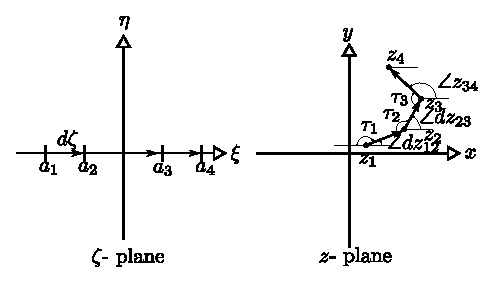
\includegraphics[scale=1.8]{figure/chapter5/5-1-40.eps}
%\caption{\label{fig:blue_rectangle} Rectangle}
\end{figure}
S-C T\\
\[
\frac{dz}{d\zeta} = K\left(\zeta - a_1\right)^{k_1-1}\left(\zeta - a_2\right)^{k_2-1}\cdots
\]
\begin{equation}
\begin{aligned}
\Longrightarrow\angle dz - \angle d\zeta 
&= \angle K + \left(k_1-1\right)\angle \left(\zeta-a_1\right) \\ 
&+ \left(k_2-1\right)\angle \left(\zeta-a_2\right) + \cdots
\end{aligned}
\tag{$\ast$}
\label{eq: 5-3-5-*}
\end{equation}
\begin{enumerate}[label = \protect\circled{\arabic*}]
\item $\zeta$ is between $\zeta = a_1$ and $\zeta = a_2$\\
\begin{align*}
\Longrightarrow \angle d\zeta =  0&& \text{ and } && \angle\left(\zeta-a_1\right) = 0,\angle\left(\zeta-a_2\right)=\angle\left(\zeta-a_3\right) =\cdots = \pi
\end{align*}
Between $z_1$ and $z_2$, from \eqref{eq: 5-3-5-*}
\[
\Longrightarrow
\angle dz_{12} - 0 = \angle K + \pi\sum_{i=2}^N\left(k_i-1\right) = \text{ constant}
\]
So segment from $z_1$ and $z_2$ is a \emph{straight line}.
\item $\zeta$ is between $\zeta = a_2$ and $\zeta = a_3$\\
\[
\angle\left(\zeta-a_1\right)=\angle\left(\zeta-a_2\right)=0
\]
\[
\angle\left(\zeta-a_3\right) = \angle\left(\zeta-a_4\right) = \cdots = \pi
\]
\begin{align*}
\eqref{eq: 5-3-5-*}\Longrightarrow
\angle dz_{23} - 0
&= \angle K + \pi\sum_{i=3}^N\left(k_i-1\right) = \text{ constant} \\
&= \angle K + \pi\sum_{i=2}^N\left(k_i-1\right) - \pi\left(k_2-1\right) \\
&= \angle dz_{12} - \pi\left(k_2-1\right)
\end{align*}
\[
\Longrightarrow\angle dz_{23} - \angle dz_{12} = -\pi\left(k_2-1\right) = \pi -\tau_2
\]
\[
\Longrightarrow\boxed{k_2=\frac{\tau_2}{\pi}}
\]
\begin{center}
\begin{tikzpicture}
\coordinate (O) at (0,0);
\node[below left] at (O) {$O$};
\fill[color=black] (O) circle[radius=2pt] ;
\coordinate (z2) at (3,2);
\node[below right] at (z2) {$z_2$};
\fill[color=black] (z2) circle[radius=2pt] ;
\coordinate (z3) at (1,5);
\node[below left] at (z3) {$z_3$};
\fill[color=black] (z3) circle[radius=2pt] ;
\draw [color=black,-{Latex[length=3mm]}, rotate=0] (O) -- (z2) ;
\draw [color=black,-{Latex[length=3mm]}, rotate=0] (z2) -- (z3) ;
\coordinate (z2dash) at (4.5,3);
\draw [dashed] (z2) -- (z2dash) ;
\draw pic["$dz_{23}-dz_{12}=-\pi\left(k_2-1\right)=\pi - \tau_2$", draw=red, text=red, ->, angle eccentricity=1.4, angle radius=1.0cm] {angle=z2dash--z2--z3};
\draw pic["$\tau_2$", draw=red, text=red, <-, angle eccentricity=1.4, angle radius=0.7cm] {angle=z3--z2--O};
\end{tikzpicture}
\end{center}
\begin{example}{For a Pentagon, the S-C T is }
\begin{figure}[H]
\centering
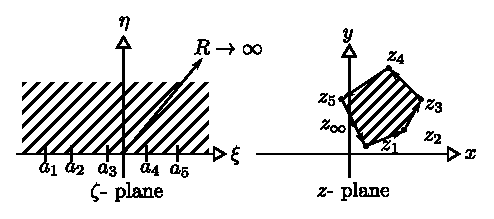
\includegraphics[scale=1.8]{figure/chapter5/5-1-41.eps}
%\caption{\label{fig:blue_rectangle} Rectangle}
\end{figure}
\[
\frac{dz}{d\zeta} = K\left(\zeta-a_1\right)^{k_1-1}\left(\zeta-a_2\right)^{k_2-1}\cdots\left(\zeta-a_5\right)^{k_5-1}
\]
The points $\infty$ on $\zeta$- plane, say $\zeta = Re^{i\varphi}$ ($R\to\infty$), will map to a \emph{point} $z_\infty$ on $z$- plane. \\
From \eqref{eq: 5-3-60}
\begin{align*}
\frac{dz}{d\zeta} 
&= K\zeta^{k_1-1}\zeta^{k_2-1}\cdots\zeta^{k_N-1} \\
&\left(1-\frac{a_1}{\zeta}\right)^{k_1-1}\left(1-\frac{a_2}{\zeta}\right)^{k_2-1}\cdots\left(1-\frac{a_N}{\zeta}\right)^{k_N-1}\\
&= K\zeta^{\sum_{i=1}^N\left(k_i-1\right)}\left[1-\frac{\sum_{i=1}^N\left(k_i-1\right)}{\zeta}+\mathcal{O}(\frac{1}{\zeta^2})\right]
\end{align*}
Integral $\Longrightarrow$
\[
z = K\frac{\zeta^{1+\sum_{i=1}^N\left(k_i-1\right)}}{1 + \sum_{i=1}^N\left(k_i-1\right)}\left[1+\mathcal{O}(\frac{1}{\zeta})\right] + C
\]
but 
\begin{align*}
1 + \sum_{i=1}^N\left(k_i-1\right)
&= 1 + \sum_{i=1}^N\left(\frac{\tau_i}{\pi} - 1\right) = 1-N+\sum_{i=1}^N\frac{\tau_i}{\pi} \\
&= 1-N+\left[\frac{\left(N-2\right)\pi}{\pi}\right] = -1
\end{align*}
\begin{equation}
\therefore z = K\left(-\frac{1}{\zeta}\right)\left[1 + \mathcal{O}(\frac{1}{\zeta})\right] + C
\label{eq: 5-3-62}
\end{equation}
hence as $\zeta\to\infty$, $z\to C$
\end{example}
\item The action of $K$ in $\displaystyle\frac{dz}{d\zeta}$ is to magnify $K=\sigma e^{i\psi}$ and rotate the polygon on $z$- plane
\end{enumerate}
\item Some considerations in constructing the S-C T\\
Q: Given $z_1,z_2,\cdots, z_N$, (and hence $\tau_1,\tau_2,\cdots,\tau_N$), how to choose $a_1,a_2,\cdots,a_N$?
\end{itemize}
\begin{note}\mbox{}\\
integrate $\eqref{eq: 5-3-60}$
\begin{equation}
\Longrightarrow z = K\int_{a_1}^{\zeta}\left(\zeta-a_1\right)^{k_1-1}\left(\zeta-a_2\right)^{k_2-1}\cdots\left(\zeta-a_N\right)^{k_N-1}d\zeta + z_1
\label{eq: 5-3-63}
\end{equation}
\underline{Observations:}
\begin{enumerate}[label = \protect\circled{\arabic*}]
\item $a_1$ is arbitrary
\item Having chosen $a_1$, \eqref{eq: 5-3-63} becomes
\begin{align*}
z_2 - z_1
&= K\int_{a_1}^{a_2}\left(\zeta-a_1\right)^{k_1-1}\left(\zeta-a_2\right)^{k_2-1}\cdots\left(\zeta-a_N\right)^{k_N-1}d\zeta \\
&= KF_2\left(a_2,a_3,\cdots,a_N\right)\\
z_3 - z_2
&= K\int_{a_2}^{a_3}\left(\zeta-a_1\right)^{k_1-1}\left(\zeta-a_2\right)^{k_2-1}\cdots\left(\zeta-a_N\right)^{k_N-1}d\zeta \\
&= KF_3\left(a_2,a_3,\cdots,a_N\right) \\
&\vdots \\
z_N - z_{N-1}
&= K\int_{a_{N-1}}^{a_N}\left(\zeta-a_1\right)^{k_1-1}\left(\zeta-a_2\right)^{k_2-1}\cdots\left(\zeta-a_N\right)^{k_N-1}d\zeta \\
&= KF_N\left(a_2,a_3,\cdots,a_N\right)
\end{align*}
where are $N-1$ constraints and $N-1$ equations (redundant: $z_1-z_N$)\\
but have $N$ unknowns, $a_2,a_3,\cdots,a_N,N$ hence another, say $a_2$, can be chosen arbitrary. Only $N-2$ constraints, not $N-1$, hence still another, say $a_3$, can be chosen arbitrary. 
\begin{conclusion}
Among $a_1$ and $a_N$ can arbitrary choose 3 of them (say $a_1,a_2,a_3$). Since arbitrary, for convenience, can take on of then, say $\boxed{a_1}\to -\infty$
\begin{align*}
\frac{dz}{d\zeta}
&= K\left(-a\right)^{k_1-1}\cancel{\left(1-\frac{\zeta}{a_1}\right)^{k_1-1}}\left(\zeta-a_2\right)^{k_2-1}\cdots \\
&= K\left(-a\right)^{k_1-1}\left(\zeta-a_2\right)^{k_2-1}\left(\zeta-a_3\right)^{k_3-1}\cdots \\
&= K'\left(\zeta-a_2\right)^{k_2-1}\left(\zeta-a_3\right)^{k_3-1}\cdots
\end{align*}
\end{conclusion}
\end{enumerate}
\end{note}
\chapter{Elements of Thin-Airfoil Theory (Linearized 2D Potential Flow)}
Assume airfoil is \emph{thin} and \emph{elongated}.
\section{Perturbation Flow- Small Perturbation Theory (Thin-Airfoil Approximation)}
\subsection{Thin airfoil assumption}
\begin{figure}[H]
\centering
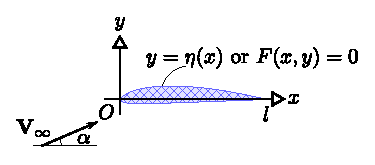
\includegraphics[scale=1.8]{figure/chapter6/6-1-1.eps}
%\caption{\label{fig:blue_rectangle} Rectangle}
\end{figure}
\begin{align*}
\alpha\ll 1, \abs{\eta(x)}\ll 1&&\text{or}&&\eta/l\ll 1,\alpha \ll 1
\end{align*}
Governing equation is
\begin{equation}
\nabla^\Phi = \frac{\partial^2\Phi}{\partial x^2} + \frac{\partial^2\Phi}{\partial y^2} = 0
\label{eq: 6-1-1}
\end{equation}
Boundary conditions are
\begin{subequations}
\begin{align}
\mathbf{v}\cdot\nabla F = 0 && \text{on $F(x,y)=0$} \label{eq: 6-1-2a}\\
\nabla\Phi\to V_\infty &&\text{at $\infty$}\label{eq: 6-1-2b}
\end{align}
\end{subequations}
\begin{align}
\text{+ KC(Kutta condition)}\colon&&\left(\nabla\Phi\right)_{\text{TE}}\text{ is finite and continuous}\label{eq: 6-1-3}
\end{align}
\begin{itemize}
\item Perturbations\\
Since $\alpha\ll 1$, $\abs{\eta}\ll 1$, can split the flow into
\begin{align*}
\mathbf{v}=\mathbf{V}_\infty + \mathbf{v'} &&\text{except }\abs{\mathbf{v'}}\ll 1
\end{align*}
where $\mathbf{v'}$ is perturbation velocity\\
i.e.
\begin{align*}
u = V_\infty\cos\alpha + u', &&v = V_\infty\sin\alpha + v'
\end{align*}
Define perturbation potential to be $\mathbf{v'}=\nabla\phi$\\
hence $\Phi = \Phi_\infty + \phi$
\[
\nabla^2\Phi = 0\Longrightarrow\nabla^2\left(\Phi_\infty+\phi\right) = 0\Longrightarrow\nabla^2\phi = 0
\]
\begin{equation}
\therefore\nabla^2\phi \equiv\frac{\partial^2\phi}{\partial x^2} + \frac{\partial^2\phi}{\partial y^2} = 0
\label{eq: 6-1-4}
\end{equation}
Boundary conditions are
\begin{subequations}
\begin{align}
\left(\mathbf{V_\infty} + \nabla\phi\right)\cdot\nabla F = 0 && \text{on $F(x,y)=0$} \label{eq: 6-1-5a}\\
\nabla^2\phi\to 0 && \text{at $\infty$}\label{eq: 6-1-5b}
\end{align}
\end{subequations}
\begin{align}
\text{+ KC(Kutta condition)}\colon&&\left(\nabla\phi\right)_{\text{TE}}\text{ is finite and continuous}\label{eq: 6-1-6}
\end{align}
\end{itemize}
\subsection{Linearized Boundary Condition}
From B.C. \eqref{eq: 6-1-5a}
\[
\left(\mathbf{V_\infty} + \nabla\phi\right)\cdot\nabla F = 0
\]
\begin{equation}
\Longrightarrow\left(V_\infty\cos\alpha+u'\right)\frac{\partial F}{\partial x} + \left(V_\infty\sin\alpha+v'\right)\frac{\partial F}{\partial y} = 0 \text{ on }F(x,y) = 0
\label{eq: 6-1-7}
\end{equation}
From now on we drop prime $'$ and the subscript represent perturbation term. 
\begin{figure}[H]
\centering
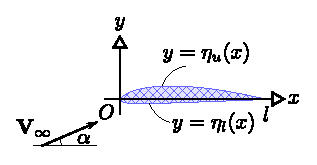
\includegraphics[scale=1.8]{figure/chapter6/6-1-2.eps}
%\caption{\label{fig:blue_rectangle} Rectangle}
\end{figure}
\begin{equation}
\eqref{eq: 6-1-7}\Longrightarrow
\frac{V_\infty\sin\alpha+ v}{V_\infty\cos\alpha+u} = \frac{-\frac{\partial F}{\partial x}}{\frac{\partial F}{\partial y}} \vc{=}{\footnotemark}{} \left(\frac{dy}{dx}\right)_{\text{body}} \equiv \frac{d\eta}{dx}
\label{eq: 6-1-9}
\end{equation}
\footnotetext{$\displaystyle dF = \frac{\partial F}{\partial x}dx + \frac{\partial F}{\partial y}dy = 0$}
(flow tangency condition on airfoil surface)
\begin{itemize}
\item Small Perturbation assumption\\
Since $\abs{\eta(x)}\ll 1$, $\alpha\ll 1$ expect velocities $u$ and $v$ be \emph{small}, i.e.
\[
\frac{u}{V_\infty},\frac{v}{V_\infty}\ll 1
\]
therefore
\begin{align*}
V_\infty\cos\alpha &\approx  V_\infty + \mathcal{O}(\alpha^2) \\
V_\infty\sin\alpha &\approx  V_\infty\alpha + \mathcal{O}(\alpha^2)
\end{align*}
\[
\eqref{eq: 6-1-9}\Longrightarrow\frac{v+V_\infty\alpha}{V_\infty}\approx\frac{d\eta}{dx}\Longrightarrow
\]
\begin{equation}
v(x,\eta)\approx V_\infty\frac{d\eta}{dx} - V_\infty\alpha\text{ on }y=\eta(x), 0\leq x\leq l
\label{eq: 6-1-10}
\end{equation}
\[
v(x,\eta) = v(x,0) + \cancel{\underbrace{\left(\frac{\partial v}{\partial y}\right)_{y=0}\eta}_{\approx \mathcal{O}(\eta^2)}}+\mathcal{O}(\eta^2)
\]
hence
\begin{align}
v(x,0)\approx V_\infty\frac{d\eta}{dx} - V_\infty\alpha, && 0\leq x\leq l
\label{eq: 6-1-11}
\end{align}
(transfer of B.C.'s)\\
for non-symmetry geometry, \eqref{eq: 6-1-11} becomes
\begin{subequations}
\begin{align}
v(x,0^+) &= V_\infty\frac{d\eta_u}{dx} - V_\infty\alpha \\
v(x,0^-) &= V_\infty\frac{d\eta_l}{dx} - V_\infty\alpha
\end{align}
for $0\leq x \leq l$
\end{subequations}
\end{itemize}
\subsection{Linearized Pressure Coefficient}
\[
p(x,y) = p_\infty + \frac{\rho}{2}V_\infty^2\left(1-\frac{V^2}{V_\infty^2}\right)
\]
where $V^2 = \left(V_\infty\cos\alpha+u\right)^2 + \left(V_\infty\sin\alpha+v\right)^2$
\[
\Longrightarrow p =p_\infty - \frac{\rho V_\infty^2}{2}\left(2\frac{u}{V_\infty}\cancelto{1}{\cos\alpha} + \frac{2v}{V_\infty}\cancelto{0}{\sin\alpha} + \cancelto{0}{\frac{u^2+v^2}{V_\infty^2}}\right)
\]
\[
\Longrightarrow p\approx p_\infty - \rho V_\infty u
\]
\[
\Longrightarrow C_p = \frac{p-p_\infty}{\frac{\rho}{2}V_\infty^2}
\]
\begin{equation}
\Longrightarrow C_p\approx-\frac{2u}{V_\infty} = -\frac{2}{V_\infty}\frac{\partial\phi}{\partial x}
\label{eq: 6-1-13}
\end{equation}
\subsection{Framework of the Thin-Airfoil Theory}
G.E.
\begin{equation}
\nabla^2\phi = \frac{\partial^2\phi}{\partial x^2} + \frac{\partial^2\phi}{\partial y^2} = 0
\label{eq: 6-1-14}
\end{equation}
B.C's
\begin{subequations}
\label{eq: 6-1-15}
\begin{align}
v(x,0^+) &= \left(\frac{\partial\phi}{\partial y}\right)_{x,0^+} = V_\infty\frac{d\eta_u}{dx} - V_\infty\alpha \label{eq: 6-1-15a}\\
v(x,0^-) &= \left(\frac{\partial\phi}{\partial y}\right)_{x,0^-} = V_\infty\frac{d\eta_l}{dx} - V_\infty\alpha \label{eq: 6-1-15b}
\end{align}
for $0\leq x \leq l$
\end{subequations}
\begin{align}
\frac{\partial\phi}{\partial x},\frac{\partial\phi}{\partial y}\to 0&&\text{as}&&x,y\to\infty
\label{eq: 6-1-16}
\end{align}
K.C.
\begin{equation}
\left(\frac{\partial\phi}{\partial x}\right)_{\text{TE}},\left(\frac{\partial\phi}{\partial y}\right)_{\text{TE}}\text{ are \emph{finite} and \emph{continuous} at TE}
\label{eq: 6-1-17}
\end{equation}
From the geometry linearlization\\
introduce a camberline function $\eta_c$
\begin{equation}
\eta_c = \frac{1}{2}\left(\eta_u+\eta_l\right)
\label{eq: 6-1-18}
\end{equation}
and thickness function $\eta_t$
\begin{equation}
\eta_t = \frac{1}{2}\left(\eta_u-\eta_l\right)
\label{eq: 6-1-19}
\end{equation}
from \eqref{eq: 6-1-18} and \eqref{eq: 6-1-19}
\begin{equation}
\begin{aligned}
\eta_u &= \eta_c + \eta_t \\
\eta_l &= \eta_c - \eta_t
\end{aligned}
\label{eq: 6-1-20}
\end{equation}
B.C. \eqref{eq: 6-1-15} becomes
\begin{subequations}
\label{eq: 6-1-21}
\begin{align}
v(x,0^+) &= \left(\frac{\partial\phi}{\partial y}\right)_{x,0^+} =  - V_\infty\alpha + V_\infty\left(\frac{d\eta_c}{dx}+\frac{d\eta_t}{dx}\right) \label{eq: 6-1-21a}\\
v(x,0^-) &= \left(\frac{\partial\phi}{\partial y}\right)_{x,0^-} =  - V_\infty\alpha + V_\infty\left(\frac{d\eta_c}{dx}-\frac{d\eta_t}{dx}\right) \label{eq: 6-1-21b}
\end{align}
for $0\leq x \leq l$
\end{subequations}
\begin{enumerate}[label = \protect\circled{\arabic*}]
\item flow past a zero-thickness flat plate at an angle-of-attack $\alpha$ 
\item flow past a zero-thickness camber at zero angle-of-attack
\item flow past a symmetric thickness airfoil at zero angle-of-attack
\end{enumerate}
\begin{figure}[H]
\centering
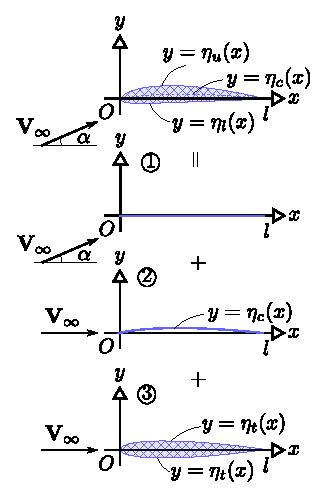
\includegraphics[scale=1.8]{figure/chapter6/6-1-3.eps}
%\caption{\label{fig:blue_rectangle} Rectangle}
\end{figure}
\section{Solutions to Elementary Thin Airfoil Problems}
\subsection{Symmetric Airfoil at Zero Angle of Attack- solution by source/sink Distribution}
\begin{itemize}
\item Governing equation
\begin{equation}
\nabla^2\phi = 0
\label{eq: 6-2-1}
\end{equation}
\begin{subequations}
\label{eq: 6-2-2}
\begin{align}
v(x,0^{\pm}) &= \left(\frac{\partial\phi}{\partial y}\right)_{x,0^{\pm}} =  \pm  V_\infty\frac{d\eta_t}{dx},0\leq x\leq l \label{eq: 6-1-2a}\\
\nabla\phi &\to 0\text{ as }x,y\to 0 \label{eq: 6-1-2b}
\end{align}
\end{subequations}
\begin{figure}[H]
\centering
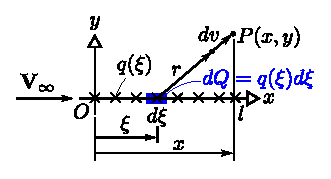
\includegraphics[scale=1.8]{figure/chapter6/6-1-4.eps}
%\caption{\label{fig:blue_rectangle} Rectangle}
\end{figure}
\begin{align}
\phi(x,y) 
&= \int d\phi = \int\frac{dQ}{2\pi}\ln r \nonumber\\
&= \frac{1}{2\pi}\int_{\xi=0}^lq(\xi)\ln\sqrt{\left(x-\xi\right)^2+y^2}d\xi\label{eq: 6-2-3}
\end{align}
and perturbation velocities $u,v$ are
\begin{subequations}
\label{eq: 6-2-4}
\begin{align}
u = \frac{\partial\phi}{\partial x} = \frac{1}{2\pi}\int_0^lq(\xi)\frac{x-\xi}{\left(x-\xi\right)^2+y^2}d\xi \label{eq: 6-2-4a}\\
v = \frac{\partial\phi}{\partial y} = \frac{1}{2\pi}\int_0^lq(\xi)\frac{y}{\left(x-\xi\right)^2+y^2}d\xi \label{eq: 6-2-4b}
\end{align}
\end{subequations}
The unknown strength $q(x)$ can be determined from the B.C. \eqref{eq: 6-1-2a}
\begin{equation}
\begin{aligned}
v(x,0^{\pm}) &= \lim_{y\to 0^\pm}\left[\frac{1}{2\pi}\int_0^lq(\xi)\frac{y}{\left(x-\xi\right)^2+y^2}d\xi\right]\\ 
&= \pm V_\infty\frac{d\eta_t}{dx}\phantom{-}(0\leq x\leq 1)
\end{aligned}
\label{eq: 6-2-5}
\end{equation}
which is \emph{Integral equation}\\
For upper surface equation \eqref{eq: 6-2-5}
\begin{align*}
v(x,0^+)
&\vc{=}{\footnotemark}{}\frac{1}{2\pi}\left\{\lim_{y\to 0^+}\left[\cancel{\int_0^{x-\delta}} + \cancel{\int_{x-\delta}^l} + \int_{x-\delta}^{x+\delta}\right]\frac{yq(\xi)}{\left(x-\xi\right)^2+y^2}d\xi\right\} \\
&=\frac{1}{2\pi}\left[\lim_{y\to 0^+}\int_{x-\delta}^{x+\delta}\frac{yq(\xi)}{\left(x-\xi\right)^2+y^2}d\xi\right]
\end{align*}
\footnotetext{for small positive $\delta$}
First, shift origin to point $x$, i.e. $\xi=x+\bar{\xi}$
\begin{align}
v(x,0^+) = \frac{1}{2\pi}\left[\lim_{y\to 0^+}\int_{\bar{\xi}= -\delta}^{\delta}\frac{yq(x+\bar{\xi})}{\bar{\xi}^2+y^2}d\bar{\xi}\right], \abs{\bar{\xi}}\ll 1
\label{eq: 6-2-6}
\end{align}
then re-scale the variable $\bar{\xi}$, i.e. let $\sigma = \bar{\xi}/y\sim\mathcal{O}(1)$
\begin{align*}
\Longrightarrow v(x,0^+) 
&= \frac{1}{2\pi}\left[\lim_{y\to 0^+}\int_{-\delta/y}^{\delta/y}\frac{q(x+y\sigma)}{\sigma^2+1}d\sigma\right] \\
&\vc{=}{\footnotemark}{y\ll 1} \frac{1}{2\pi}\lim_{y\to 0^+}\left\{\int_{-\delta/y}^{\delta/y}\frac{q(x)}{\sigma^2+1}d\sigma + y\int_{-\delta/y}^{\delta/y}\frac{q'(x)\sigma}{\sigma^2+1}d\sigma\right\} + \cdots \\
&= \frac{q(x)}{2\pi}\left\{\lim_{y\to 0^+}\int_{-\delta/y}^{\delta/y}\frac{d\sigma}{\sigma^2+1}\right\} \\
&= \frac{q(x)}{2\pi}\left\{\lim_{y\to 0^+}\left[\arctan\sigma\right]_{-\delta/y\to\infty}^{\delta/y\to -\infty}\right\} \\
&= \frac{q(x)}{2}
\end{align*}
\footnotetext{hence $q(x+y\sigma) = q(x) + q'(x)y\sigma + \mathcal{O}(y^2)$} 
Similarly, 
\[
v(x,0^-) = -\frac{q(x)}{2}
\]
i.e.
\begin{equation}
q(x) = 2v(x,0^+) = 2V_\infty\frac{d\eta_t}{dx}
\label{eq: 6-2-7}
\end{equation}
Having known the $q(x)$
\begin{align*}
\Longrightarrow u(x,y)=?, && v(x,y) = ?
\end{align*}
The pressure coefficient $C_p(x,y)$ is 
\begin{equation}
C_p(x,y) = -\frac{2u(x,y)}{V_\infty}
\label{eq: 6-2-8}
\end{equation}
Specifically, the $C_p$ on the surface of the airfoil is
\begin{subequations}
\label{eq: 6-2-9}
\begin{equation}
C_p(x,0^{\pm}) = -\frac{2u(x,0^{\pm})}{V_\infty}
\label{eq: 6-2-9a}
\end{equation}
with 
\begin{align}
u(x,0)
&= \frac{1}{2\pi}\left\{\int_{\xi=0}^lq(\xi)\frac{x-\xi}{\left(x-\xi\right)^2+y^2}d\xi\right\}_{y=0} \nonumber \\
&= \frac{1}{2\pi}\int_0^l\frac{q(\xi)}{x-\xi}d\xi = \frac{V_\infty}{\pi}\int_{\xi=0}^l\frac{d\eta_t(\xi)}{d\xi}\frac{1}{x-\xi}d\xi
\label{eq: 6-2-9b}
\end{align}
\end{subequations}
(Hilbert integral)\\
Often, transform $x,\xi$ into $\theta,\varphi$ by using
\begin{equation}
\begin{aligned}
x&=\frac{l}{2}\left(1+\cos\theta\right),  0\leq \theta\leq \pi(\text{upper}), -\pi\leq \theta\leq 0(\text{lower}) \\
\xi &= \frac{l}{2}\left(1+\cos\varphi\right),  0\leq \varphi\leq \pi(\text{upper}), -\pi\leq \varphi\leq 0(\text{lower})
\end{aligned}
\end{equation}
\begin{figure}[H]
\centering
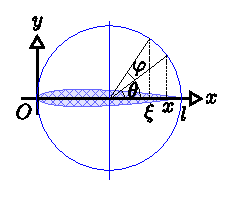
\includegraphics[scale=1.8]{figure/chapter6/6-1-5.eps}
%\caption{\label{fig:blue_rectangle} Rectangle}
\end{figure}
then \eqref{eq: 6-2-9b} becomes Poisson's Integral Formula
\begin{align}
u(\theta)
&= -\frac{1}{2\pi}\int_{\varphi = \pi}^0q(\varphi)\frac{\sin\varphi}{\cos\theta-\cos\varphi}d\varphi \nonumber\\
&= -\frac{1}{2\pi}\int_0^\pi q(\varphi)\frac{\sin\varphi}{\cos\varphi-\cos\theta}d\varphi \label{eq: 6-2-12} \\
&= -\frac{V_\infty}{\pi}\int_0^\pi\frac{d\eta_t(\varphi)}{d\xi}\frac{\sin\varphi}{\cos\varphi-\cos\theta}d\varphi \label{eq: 6-2-13}
\end{align}
(Poisson's Integral Formula)\\
notations:\\
\[
u(\theta)\equiv u(x(\theta),0^{\pm})
\]
\[
\frac{\partial\eta_+(\theta)}{dx} = \left.\frac{\partial\eta_+(x)}{dx}\right|_{x=x(\theta)}
\]
\item The pressure coefficient $C_p$ on the surface of the airfoil\\
Since $\displaystyle\frac{d\eta_t}{dx}$ (odd function in $x$ by expanding $\displaystyle\frac{d\eta_t}{dx}$ into a Fourier Sine Series), using $\displaystyle x=\frac{l}{2}\left(1+\cos\theta\right)$
\begin{equation}
\frac{d\eta_t(\theta)}{dx} = \sum_{n=1}^\infty A_n\sin n\theta\label{eq: 6-2-14}
\end{equation}
where
\begin{equation}
A_n = \frac{2}{\pi}\int_0^\pi\frac{d\eta_t(\theta)}{dx}\sin n\theta d\theta \label{eq: 6-2-15}
\end{equation}
then \eqref{eq: 6-2-13} becomes
\begin{equation}
\frac{u(\theta)}{V_\infty} = -\frac{1}{\pi}\int_0^\pi\underbrace{\left(\sum_{n=1}^\infty A_n\sin n\varphi\right)}_{\text{Given}}\underbrace{\frac{\sin\varphi}{\cos\varphi - \cos\theta}}_{\text{Kernal}}d\varphi
\label{eq: 6-2-16}
\end{equation}
Now what is $\displaystyle\int_0^\pi\frac{\sin n\varphi \sin\varphi}{\cos\varphi-\cos\theta}d\varphi=?$
first
\[
\sin n\varphi \sin\varphi = -\frac{1}{2}\left[\cos(n+1)\varphi - \cos(n+1)\varphi\right]
\]
Now define
\[
I_n(\theta) = \int_0^\pi\frac{\cos n\varphi}{\cos\varphi - \cos\theta}d\varphi
\]
\begin{enumerate}[label = \protect\circled{\arabic*}]
\item $\displaystyle I_0(\theta) = \int_0^\pi\frac{1}{\cos\varphi - \cos\theta}d\varphi = 0$
\item $\displaystyle I_1(\theta) = \int_0^\pi\frac{\cos\varphi}{\cos\varphi - \cos\theta}d\varphi = \int_0^\pi\left[1+\frac{\cos\theta}{\cos\varphi-\cos\theta}\right]d\varphi = \pi$
\item $I_2(\theta) = \cdots = 2\cos\theta I_1 = 2\pi\cos\theta$
\end{enumerate}
for general $n$
\begin{equation}
I_n = \pi\frac{\sin n\theta}{\sin\theta}
\label{eq: 6-2-19}
\end{equation}
Hence in \eqref{eq: 6-2-16}
\begin{align*}
\int_0^\pi\frac{\sin n\varphi \sin\varphi}{\cos\varphi-\cos\theta}d\varphi
&= -\frac{1}{2}\left\{\underbrace{\int_0^\pi\frac{\cos(n+1)\varphi}{\cos\varphi-\cos\theta}d\varphi}_{I_{n+1}} - \underbrace{\int_0^\pi\frac{\cos(n-1)\varphi}{\cos\varphi-\cos\theta}d\varphi}_{I_{n-1}}\right\} \\
&= -\frac{1}{2}\left[I_{n+1}-I_{n-1}\right] \\
&= -\frac{1}{2}\frac{\pi}{\sin\theta}\left[2\cos n\theta\sin\theta\right] = -\pi\cos n\theta
\end{align*}
\begin{equation}
\therefore\frac{u(\theta)}{V_\infty} = \sum_{n=1}^\infty A_n\cos n\theta
\end{equation}
where
\[
A_n = \frac{2}{\pi}\int_0^\pi\frac{d\eta_t(\theta)}{dx}\sin n\theta d\theta
\]
\begin{align}
C_p(x,0^{\pm})
&\equiv C_p(\theta)  = -\frac{2u(\theta)}{V_\infty} \nonumber\\
&= -2\sum_{n=1}^\infty A_n\cos n\theta\label{eq: 6-2-21}
\end{align}
where
\begin{align*}
0\leq\theta\leq \pi\colon && \text{upper surface}
\end{align*}
\begin{align*}
-\pi\leq\theta\leq 0\colon && \text{lower surface}
\end{align*}
\end{itemize}
\subsection{Cambered Airfoil at zero Angle-of-Attack- solution by vortices Distribution (Vortex sheet)}
\begin{figure}[H]
\centering
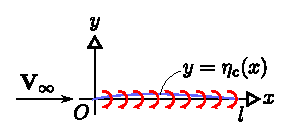
\includegraphics[scale=1.8]{figure/chapter6/6-1-6.eps}
%\caption{\label{fig:blue_rectangle} Rectangle}
\end{figure}
\begin{itemize}
\item Governing equation
\begin{equation}
\nabla^2\phi = 0
\label{eq: 6-2-25}
\end{equation}
\begin{subequations}
\label{eq: 6-2-26}
\begin{align}
v(x,0^{\pm}) &= \left(\frac{\partial\phi}{\partial y}\right)_{x,0^{\pm}} =   V_\infty\frac{d\eta_c}{dx},0\leq x\leq l \label{eq: 6-2-26a}\\
\nabla\phi &\to 0\text{ as }x,y\to 0 \label{eq: 6-2-26b}
\end{align}
\end{subequations}
K.C.
\begin{equation}
u=\frac{\partial\phi}{\partial x},v=\frac{\partial\phi}{\partial y}\text{ is finite and continuous at TE}
\label{eq: 6-2-27}
\end{equation}
\begin{figure}[H]
\centering
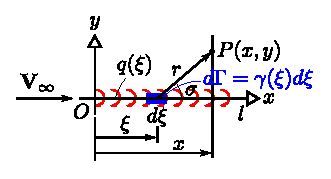
\includegraphics[scale=1.8]{figure/chapter6/6-1-7.eps}
%\caption{\label{fig:blue_rectangle} Rectangle}
\end{figure}
\begin{align}
\phi(x,y)
&= \int d\phi = \int -\frac{d\Gamma}{2\pi}\sigma = -\frac{1}{2\pi}\int_{\xi=0}^l\gamma(\xi)\sigma d\xi \nonumber \\
&= -\frac{1}{2\pi}\int_0^l\gamma(\xi)\arctan\frac{y}{x-\xi} d\xi \label{eq: 6-2-28}
\end{align}
velocities $u,v$
\begin{subequations}
\label{eq: 6-2-29}
\begin{align}
u(x,y) &= \frac{\partial\phi}{\partial x} = \frac{1}{2\pi}\int_0^l\gamma(\xi)\frac{y}{\left(x-\xi\right)^2+y^2}d\xi \label{eq: 6-2-29a}\\
v(x,y) &= \frac{\partial\phi}{\partial y} = \frac{1}{2\pi}\int_0^l\gamma(\xi)\frac{x-\xi}{\left(x-\xi\right)^2+y^2}d\xi \label{eq: 6-2-29b}
\end{align}
\end{subequations}
Now what is $\gamma(x)$ ?\\
look at $u(x,0^{\pm})$ first
\begin{equation}
\eqref{eq: 6-2-29a}\Longrightarrow
u(x,0^{\pm}) = \lim_{y\to 0^{\pm}}\left[\frac{1}{2\pi}\underbrace{\int_0^l\gamma(\xi)\frac{y}{\left(x-\xi\right)^2 + y^2}d\xi}_{\text{Improper integral}}\right]
\tag{$\ast$} \label{eq: 6-2-2-*}
\end{equation}
Again, an improper integral\\
<cf> \eqref{eq: 6-2-5},\eqref{eq: 6-2-6}$\Longrightarrow v(x,0^{+}) = q(x)/2$\\
Hence \eqref{eq: 6-2-2-*} becomes
\begin{subequations}
\label{eq: 6-2-30}
\begin{align}
u(x,0^+) &= \frac{\gamma(x)}{2} \label{eq: 6-2-30a}\\
u(x,0^-) &= -\frac{\gamma(x)}{2} \label{eq: 6-2-30b}
\end{align}
\end{subequations}
\begin{equation}
\eqref{eq: 6-2-30a},\eqref{eq: 6-2-30b}\Longrightarrow\gamma(x) = u(x,0^+)-u(x,0^-)
\label{eq: 6-2-31}
\end{equation}
From \eqref{eq: 6-2-31}, deduce
\begin{equation}
\text{KC }\Longrightarrow\gamma(x=l) = 0
\label{eq: 6-2-32}
\end{equation}
The pressure coefficient $C_p$ on the camber surface
\begin{equation}
C_p(x,0^{\pm}) = -\frac{2u(x,0^\pm)}{V_\infty} = \mp\frac{\gamma(x)}{V_\infty}
\end{equation}
where $+$ is \emph{upper surface} and $-$ is \emph{lower surface}
The lift force on the camber airfoil 
\begin{align*}
L 
&= \int_0^l\left[p(x,0^-)-p(x,0^+)\right]dx \\
&= \frac{\rho}{2}V_\infty^2\int_0^l\left[C_p(x,0^-)-C_p(x,0^+)\right]dx \\
&=\rho V_\infty\int_0^l\gamma(x)dx=\rho V_\infty\Gamma
\end{align*}
The moment (about $x=0$) on the camber airfoil is
\begin{align}
M
&= \int_0^l\left[p(x,0^+)-p(x,0^-)\right]xdx \nonumber\\
&= -\rho V_\infty\int_0^l\gamma(x)xdx\label{eq: 6-2-35}
\end{align}
lift and moment coefficients
\begin{equation}
C_L = \frac{L}{\frac{\rho}{2}V_\infty^2l} = \frac{2}{V_\infty l}\int_0^l\gamma(x)dx
\label{eq: 6-2-36}
\end{equation}
\begin{equation}
C_M = \frac{M}{\frac{\rho}{2}V_\infty^2l^2} = \frac{-2}{V_\infty l^2}\int_0^l\gamma(x)xdx
\label{eq: 6-2-37}
\end{equation}
Now $\gamma(x)$ has to be determined from B.C. \eqref{eq: 6-2-26a}
\begin{align}
v(x,0^\pm) 
&= \lim_{y\to 0^\pm} \left[-\frac{1}{2\pi}\int_0^l\gamma(\xi)\frac{x-\xi}{\left(x-\xi\right)^2+y^2}d\xi\right] = \underbrace{V_\infty\frac{d\eta_c}{dx}}_{\text{Given}}\phantom{-}(0\leq x\leq l) \nonumber\\
&= - \frac{1}{2\pi}\int_0^l\gamma(\xi)\frac{d\xi}{x-\xi} = V_\infty\frac{d\eta_c}{dx}\phantom{-}(0\leq x\leq l) \label{eq: 6-2-38}
\end{align}
(Singular integral/Hilbert integral)
\item As before; can transform $x,\xi$ into $\theta,\varphi$ by
\begin{alignat*}{4}
& x = \frac{l}{2}\left(1+\cos\theta\right)     \quad && 0\leq\theta,\varphi\leq\pi \quad && \colon \quad && \text{upper surface}\\
& \xi = \frac{l}{2}\left(1+\cos\varphi\right)     \quad && -\pi\leq\theta,\varphi\leq 0 \quad && \colon \quad && \text{lower surface}
\end{alignat*}
\begin{equation}
\eqref{eq: 6-2-38}\Longrightarrow\frac{1}{2\pi V_\infty}\int_{\varphi = 0}^\pi\underbrace{\gamma(\varphi)}_{\text{unknown}}\frac{\sin\varphi}{\cos\varphi-\cos\theta}d\varphi = \underbrace{\frac{d\eta_c(\theta)}{dx}}_{\text{Given}}
\label{eq: 6-2-41}
\end{equation}
For arbitrary shape of camber\\
Since $\displaystyle\frac{d\eta_c}{dx}$ is an even function $\Longrightarrow\displaystyle\frac{d\eta_c(\theta)}{dx}$ is an even function in $\theta$
\begin{equation}
\Longrightarrow\frac{d\eta_c(\theta)}{dx} = \frac{B_0}{2} + \sum_{n=1}^\infty B_n\cos n\theta
\label{eq: 6-2-42}
\end{equation}
where 
\begin{align*}
\underbrace{B_0 = \frac{2}{\pi}\int_0^\pi\frac{d\eta_c(\theta)}{dx}d\theta}_{\text{(average of slope)}}, &&B_n = \frac{2}{\pi}\int_0^\pi\frac{d\eta_c(\theta)}{dx}\cos n\theta d\theta
\end{align*}
Using \eqref{eq: 6-2-42}, $\eqref{eq: 6-2-41}\Longrightarrow$
\begin{equation}
\frac{1}{2\pi V_\infty}\int_0^\pi\underbrace{\gamma(\varphi)}_{\text{unknown}}\frac{\sin\varphi}{\cos\varphi-\cos\theta}d\varphi = \underbrace{\frac{B_0}{2}+\sum_{n=1}^\infty B_n\cos n\theta}_{\text{Given}}
\label{eq: 6-2-43}
\end{equation}
wish to solve $\gamma(\theta)=$?\\
Assume the solution to $\gamma(\theta)$ is
\[
\gamma(\theta) = \gamma_1(\theta) + \gamma_2(\theta) + \gamma_h(\theta)
\]
where
\begin{equation}
\frac{1}{2\pi V_\infty}\int_0^\pi\gamma_1(\varphi)\frac{\sin\varphi}{\cos\varphi - \cos\theta}d\varphi = \sum_{n=1}^\infty B_n\cos n\theta
\label{eq: 6-2-45}
\end{equation}
\begin{equation}
\frac{1}{2\pi V_\infty}\int_0^\pi\gamma_2(\varphi)\frac{\sin\varphi}{\cos\varphi - \cos\theta}d\varphi = \frac{B_0}{2}
\label{eq: 6-2-46}
\end{equation}
\begin{equation}
\frac{1}{2\pi V_\infty}\int_0^\pi\gamma_h(\varphi)\frac{\sin\varphi}{\cos\varphi - \cos\theta}d\varphi = 0
\label{eq: 6-2-47}
\end{equation}
Solution to $\gamma_1(\theta),\gamma_2(\theta),\gamma_h(\theta)$
\[
\gamma_1(\varphi) = -2V_\infty\sum_{n=1}^\infty B_n\sin n\varphi\text{ (Recall \eqref{eq: 6-2-16})}
\]
or
\begin{equation}
\gamma_1(\theta) = -2V_\infty\sum_{n=1}^\infty B_n\sin n\theta
\label{eq: 6-2-48}
\end{equation}
Recall that
\begin{align*}
I_n = \int_0^\pi\frac{\cos n\varphi}{\cos\varphi - \cos\theta}d\varphi = \pi\frac{\sin n\theta}{\sin\theta}, && n=0,1,2,\cdots
\end{align*}
which suggest
\begin{equation}
\gamma_2(\varphi) = V_\infty B_0\frac{\cos\theta}{\sin\theta}
\label{eq: 6-2-49}
\end{equation}
Also $I_0=0$, which suggest
\begin{equation}
\gamma_h(\theta) = \frac{K}{\sin\theta}
\label{eq: 6-2-50}
\end{equation}
Hence 
\begin{align}
\gamma(\theta) 
&= \gamma_1(\theta) + \gamma_2(\theta) + \gamma_h(\theta)  \nonumber\\
&= -2V_\infty\sum_{n=1}^\infty B_n\sin n\theta + \frac{V_\infty B_0}{\sin\theta}\left(\frac{\overbrace{K}^{\text{undetermined}}}{V_\infty B_0} + \cos\theta\right)
\label{eq: 6-2-51}
\end{align}
Apply K.C.
\[
\gamma(x=l) = \gamma(\theta=0)=0\Longrightarrow\left.\frac{1}{\sin\theta}\left(\frac{K}{V_\infty B_0}+\cos\theta\right)\right|_{\theta = 0} = 0
\]
\[
\Longrightarrow K = -V_\infty B_0
\]
\begin{equation}
\therefore\gamma(\theta) = -2V_\infty\left(\frac{B_0}{2}\frac{1-\cos\theta}{\sin\theta}+\sum_{n=1}^\infty B_n\sin n\theta\right)
\label{eq: 6-2-52}
\end{equation}
\item Pressure coefficient along the camber
\begin{align}
C_p(\theta)
&\equiv C_p(x(\theta),0^\pm) = -\frac{2u(x(\theta),0^\pm)}{V_\infty} \nonumber\\
&= -\frac{\gamma(\theta)}{V_\infty},0\leq \theta\leq \pi(\text{upper}), -\pi\leq \theta\leq 0(\text{lower}) \nonumber\\ 
&= B_0\frac{1-\cos\theta}{\sin\theta} + 2\sum_{n=1}^\infty B_n\sin n\theta \label{eq: 6-2-53}
\end{align}
\begin{align}
C_L
&= \frac{2}{V_\infty l}\int_{x=0}^l\gamma(x)dx, x=\frac{l}{2}\left(1+\cos\theta\right)\nonumber \\
&= \frac{1}{V_\infty}\int_{\theta=0}^\pi\gamma(\theta)\sin\theta d\theta \label{eq: 6-2-54}
\end{align}
\begin{align}
C_M 
&= -\frac{2}{V_\infty l^2}\int_{x=0}^l\gamma(x)xdx \nonumber\\ 
&= -\frac{1}{2V_\infty}\int_{\theta = 0}^\pi\gamma(\theta)\left(1+\cos\theta\right)\sin\theta d\theta
\label{eq: 6-2-55}
\end{align}
Use \eqref{eq: 6-2-52}
\begin{equation}
C_L = -\left(B_0+B_1\right)\pi
\label{eq: 6-2-56}
\end{equation}
\begin{align}
C_M 
&=B_0\frac{\pi}{4} + B_1\frac{\pi}{2} + B_2\frac{\pi}{4} \nonumber \\
&= \frac{\pi}{4}\left(B_0+B_1\right) + \frac{\pi}{4}\left(B_1+B_2\right) \nonumber \\
&= -\frac{C_L}{4} + \frac{\pi}{4}\left(B_1+B_2\right)\label{eq: 6-2-57}
\end{align}
\begin{note}
\begin{align*}
\int_0^\pi\sin n\theta \sin m\theta d\theta 
&= 0 &&\text{for }n\neq m \\
&= \frac{\pi}{2} &&\text{for }n= m
\end{align*}
\end{note}
Recall
\[
B_0 = \frac{2}{\pi}\int_0^\pi\frac{d\eta_c(\theta)}{dx}d\theta
\]
\begin{align}
B_n = \frac{2}{\pi}\int_0^\pi\frac{d\eta_c(\theta)}{dx}\cos n\theta d\theta, && \text{for }n=1,2,\cdots
\label{eq: 6-2-58}
\end{align}
\end{itemize}
\subsection{Flat-Plate Airfoil at an Angle-of-Attack $\alpha$- solution by vortices Distribution (Vortex sheet)}
\begin{itemize}
\item Governing equation
\begin{equation}
\nabla^2\phi = 0
\label{eq: 6-2-60}
\end{equation}
\begin{subequations}
\label{eq: 6-2-61}
\begin{align}
v(x,0^{\pm}) &= \left(\frac{\partial\phi}{\partial y}\right)_{x,0^{\pm}} =   -V_\infty\alpha,0\leq x\leq l \label{eq: 6-2-61a}\\
\nabla\phi &\to 0\text{ as }x,y\to 0 \label{eq: 6-2-61b}
\end{align}
\end{subequations}
K.C.
\begin{equation}
u=\frac{\partial\phi}{\partial x},v=\frac{\partial\phi}{\partial y}\text{ is finite and continuous at TE}
\label{eq: 6-2-62}
\end{equation}
\begin{figure}[H]
\centering
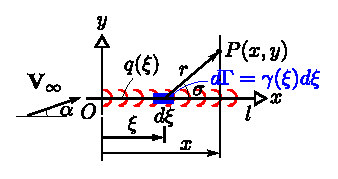
\includegraphics[scale=1.8]{figure/chapter6/6-1-8.eps}
%\caption{\label{fig:blue_rectangle} Rectangle}
\end{figure}
From previous cambered airfoil case
\begin{equation}
v(x,0^\pm) = -\frac{1}{2\pi}\int_0^l\gamma(\xi)\frac{d\xi}{x-\xi}\phantom{-}(0\leq x\leq l) 
\label{eq: 6-2-63}
\end{equation}
As before, transform $
\left\{
\begin{aligned}
&x \\
&\xi 
\end{aligned}
\right.
\Longrightarrow
\left\{
\begin{aligned}
&\theta \\
&\varphi
\end{aligned}
\right.
$
by
$
\left\{
\begin{aligned}
x&=\frac{l}{2}\left(1+\cos\theta\right) \\
\xi&=\frac{l}{2}\left(1+\cos\varphi\right)
\end{aligned}
\right.
$
\begin{equation}
\eqref{eq: 6-2-63}\Longrightarrow
v(x,0^\pm) = \frac{1}{2\pi}\int_0^l\gamma(\varphi)\frac{\sin\varphi}{\cos\varphi-\cos\theta}d\varphi = -V_\infty\alpha
\end{equation}
As before, can get $\gamma(\theta)=\gamma_2(\theta)+\gamma_h(\theta)$ <cf> \eqref{eq: 6-2-43}
\label{eq: 6-2-65}
\begin{equation}
\Longrightarrow
\gamma(\theta) = \underbrace{\frac{K}{\sin\theta}}_{\gamma_h(\theta)} - \underbrace{2V_\infty\alpha\frac{\cos\theta}{\sin\theta}}_{\gamma_2(\theta)}
\label{eq: 6-2-66}
\end{equation}
To satisfy $\gamma(\theta=0)=0\Longrightarrow K = 2V_\infty\alpha$, i.e.
\begin{equation}
\gamma(\theta) = 2V_\infty\alpha\frac{1-\cos\theta}{\sin\theta}
\label{eq: 6-2-67}
\end{equation}
\item The pressure coefficient along the flat plate 
\begin{equation}
C_p(\theta) = -\frac{\gamma(\theta)}{V_\infty} = -2\alpha\frac{1-\cos\theta}{\sin\theta}
\label{eq: 6-2-68}
\end{equation}
\begin{align*}
0\leq \theta\leq \pi\colon\text{ upper surface},&& -\pi\leq \theta\leq 0\colon\text{ lower surface}
\end{align*}
\begin{equation}
C_L = \frac{1}{V_\infty}\int_{\theta=0}^\pi\gamma(\theta)\sin\theta d\theta = 2\alpha\int_0^\pi\frac{1-\cos\theta}{\sin\theta}\sin\theta d\theta = 2\pi\alpha
\label{eq: 6-2-69}
\end{equation}
\begin{equation}
C_M = -\frac{1}{2V_\infty}\int_{\theta=0}^\pi\gamma(\theta)\left(1+\cos\theta\right)\sin\theta d\theta = -\frac{\pi}{2}\alpha = -\frac{C_L}{4}
\label{eq: 6-2-70}
\end{equation}
center of pressure
\begin{align*}
C_L = \frac{L}{\frac{\rho}{2}V_\infty^2 l}(=2\pi\alpha), &&C_M = \frac{M}{\frac{\rho}{2}V_\infty^2 l^2}(=-\frac{C_L}{4})
\end{align*}
\begin{align*}
M &= -Lx_{\text{cp}} \\
\Longrightarrow
\frac{\rho}{2}V_\infty^2l^2C_M &= \frac{\rho}{2}V_\infty^2l^2\left(-\frac{C_L}{4}\right) = -L\frac{l}{4}
\end{align*}
\begin{equation}
\therefore\boxed{x_{\text{cp}} = \frac{l}{4}}
\label{eq: 6-2-71}
\end{equation}
Aerodynamic center ($x_\text{ac}$):\\
About which the moment is independent of angle-of-attack $\alpha$. Take moment about $x=l/4$
\begin{align}
\Longrightarrow\overline{C_M} = 0&&\text{independent of }\alpha
\label{eq: 6-2-72}
\end{align}
so in the case: $x_\text{ac} = x_\text{cp} = l/4$
\end{itemize}
\subsection{Aerodynamic Characteristic of a Complete Thin Airfoil (Superposition)}
Superpose the above 3 elementary cases:\\
camber + thickness
\[
\Longrightarrow\frac{d\eta_{u,l}}{dx} = \frac{d\eta_c}{dx}\pm\frac{d\eta_t}{dx}
\]
or
\begin{equation}
\frac{d\eta(\theta)}{dx} = \frac{d\eta_c(\theta)}{dx} + \frac{d\eta_t(\theta)}{dx}, \phantom{-}\left(x=\frac{l}{2}\left(1+\cos\theta\right)\right)
\label{eq: 6-2-73}
\end{equation}
from previous results
\begin{equation}
\frac{d\eta(\theta)}{dx} = \underbrace{\frac{B_0}{2}+\sum_{n=1}^\infty B_n\cos n\theta}_{\text{camber}} + \underbrace{\sum_{n=1}^\infty A_n\sin n\theta}_{\text{thickness}}
\label{eq: 6-2-74}
\end{equation}
where
\begin{equation}
\left\{
\begin{aligned}
A_n &= \frac{2}{\pi}\int_0^\pi\frac{d\eta_t(\theta)}{dx}\sin n\theta d\theta, n=1,2,3,\cdots \\
B_0 &= \frac{2}{\pi}\int_0^\pi\frac{d\eta_c(\theta)}{dx}d\theta \\
B_n &= \frac{2}{\pi}\int_0^\pi\frac{d\eta_c(\theta)}{dx}\cos n\theta d\theta, n=1,2,3,\cdots
\end{aligned}
\right.
\label{eq: 6-2-75}
\end{equation}
Pressure distribution
\begin{align}
C_p(\theta)
&= - 2\frac{u(\theta)}{V_\infty}\nonumber \\
&= \underbrace{-2\alpha\frac{1-\cos\theta}{\sin\theta}}_{
\begin{subarray}{c}
  \text{due to flat plat}\\
  \text{at $\alpha$ angle-of-attack}
\end{subarray}
}
+
\underbrace{\left[B_0\frac{1-\cos\theta}{\sin\theta} + 2\sum_{n=1}^\infty B_n\sin n\theta\right]}_{
\begin{subarray}{c}
  \text{due to camber at}\\
  \text{zero angle-of-attack}
\end{subarray}
}
\underbrace{-2\sum_{n=1}^\infty A_n\cos n\theta}_{
\begin{subarray}{c}
  \text{due to thickness}\\
  \text{at zero angle-of-attack}
\end{subarray}
}
\label{eq: 6-2-76}
\end{align}
\begin{equation}
C_L = \underbrace{2\pi\alpha}_{
\begin{subarray}{c}
  \text{due to flat plate}\\
  \text{at $\alpha$}
\end{subarray}
}  \underbrace{-\left(B_0+B_1\right)\pi}_{
\begin{subarray}{c}
  \text{due to camber}\\
  \text{at zero}
\end{subarray}
}
\label{eq: 6-2-77}
\end{equation}
\begin{align}
C_M 
&= \underbrace{-\frac{\pi}{2}\alpha}_{
\begin{subarray}{c}
  \text{due to flat plate}\\
  \text{at $\alpha$}
\end{subarray}
} + \underbrace{\frac{\pi}{4}\left(B_0+B_1\right)+\frac{\pi}{4}\left(B_1+B_2\right)}_{
\begin{subarray}{c}
  \text{due to camber}\\
  \text{at zero}
\end{subarray}
} \nonumber \\
&= -\frac{C_L}{4}+\frac{\pi}{4}\left(B_1+B_2\right)
\label{eq: 6-2-79}
\end{align}
Take moment about $x_\text{ac} = l/4$
\begin{align}
\Longrightarrow\overline{C_M} = \frac{\pi}{4}\left(B_1+B_2\right)&&\text{independent of }\alpha
\label{eq: 6-2-80}
\end{align}
\begin{example}{a parabolic camber airfoil}
\begin{align*}
y = 4\epsilon\frac{x}{l}\left(l-x\right), &&(\epsilon\ll 1)
\end{align*}
\begin{align*}
\frac{d\eta_c}{dx}
&\equiv \frac{dy}{dx} = 4\epsilon - \frac{8\epsilon}{l}x = 4\epsilon - \frac{8\epsilon}{l}\frac{l}{2}\left(1+\cos\theta\right) \\
&=-4\epsilon\cos\theta = \frac{B_0}{2} + \sum_{n=1}^\infty B_n\cos n\theta
\end{align*}
\begin{align*}
\Longrightarrow B_0=0, && B_1 = -4\epsilon,&& B_n = 0\phantom{-}(n\geq 2)
\end{align*}
\[
C_L = 2\pi\alpha-\left(B_0+B_1\right)\pi = 2\pi\alpha + 4\epsilon\pi
\]
\[
C_M = -\frac{C_L}{4} + \frac{\pi}{4}\left(B_1+B_2\right) = -\frac{\pi\alpha}{2}-2\epsilon\pi
\]
\[
\overline{C_M} = \frac{\pi}{4}\left(B_1+B_2\right) = -\epsilon\pi\phantom{-}\text{independent of }\alpha
\]
also
\begin{align*}
\gamma(\theta)
&= 2V_\infty\alpha\frac{1-\cos\theta}{\sin\theta} - 2V_\infty\left(\frac{B_0}{2}\frac{1-\cos\theta}{\sin\theta} + \sum_{n=1}^\infty B_n\sin n\theta\right) \\
&= 2V_\infty\alpha\frac{1-\cos\theta}{\sin\theta} + 8\epsilon V_\infty\sin\theta
\end{align*}
and
\[
\Gamma = \int_{x=0}^l\gamma(x)dx = \frac{l}{2}\int_{\theta=0}^\pi\gamma(\theta)\sin\theta d\theta = \pi V_\infty l\left(\alpha +2\epsilon\right)
\]
\[
C_p(\theta) =  -2\alpha\frac{1-\cos\theta}{\sin\theta} - 8\epsilon\sin\theta
\]
\end{example}
\chapter{Three-Dimensional Potential Flows}
\begin{equation}
\left.
\begin{aligned}
\text{Incompressible}&\colon\nabla\cdot\mathbf{v}=0\\
\text{Irrotational}&\colon\nabla\times\mathbf{v}=0
\end{aligned}
\right\}
\Longrightarrow\nabla^2\Phi = 0,\mathbf{v}=\nabla\Phi
\end{equation}
\section{General Solution to 3D Axisymmetric Potential Flows}
\subsection{Governing Equations}
\begin{equation}
\nabla^2\Phi = 0
\label{eq: 7-1-1}
\end{equation}
Since axisymmetric, adopt spherical coordinate ($r,\theta,\varphi$)
\begin{figure}[H]
\centering
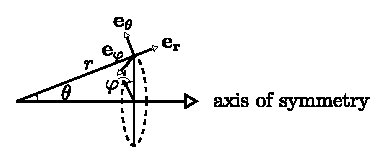
\includegraphics[scale=1.8]{figure/chapter7/7-1-1.eps}
%\caption{\label{fig:blue_rectangle} Rectangle}
\end{figure}
\begin{align*}
\nabla^2\Phi=0, &&(\frac{\partial}{\partial\varphi} = 0)
\end{align*}

\begin{equation}
\frac{1}{r^2}\frac{\partial}{\partial r}\left(r^2\frac{\partial\Phi}{\partial r}\right) + \frac{1}{r^2\sin\theta}\frac{\partial}{\partial\theta}\left(\sin\theta\frac{\partial\Phi}{\partial\theta}\right) = 0
\label{eq: 7-1-2}
\end{equation}
(Laplace equation)
\begin{itemize}
\item Stream function- Stokes' stream function\\
Recall vector potential in spherical coordinates
\[
\boldsymbol{\Psi} = \mathbf{e_\varphi}\frac{1}{r\sin\theta}\underbrace{\psi}_{
\begin{subarray}{c}
  \text{Stokes'}\\
  \text{stream function}
\end{subarray}
}
\]
where
\begin{subequations}
\label{eq: 7-1-3}
\begin{align}
v_r = \frac{1}{r^2\sin\theta}\frac{\partial\psi}{\partial\theta} \label{eq: 7-1-3a}\\
v_\theta = -\frac{1}{r\sin\theta}\frac{\partial\psi}{\partial r}\label{eq: 7-1-3b}
\end{align}
\end{subequations}
and governing equation for $\boldsymbol{\Psi}$
\begin{align*}
\nabla^2\boldsymbol{\Psi} = 0&&\text{i.e.}&&\nabla^2\left(\mathbf{e}_\varphi\frac{1}{r\sin\theta}\psi\right)=0
\end{align*}
spelling out
\begin{equation}
\Longrightarrow
\underbrace{\frac{\partial^2\psi}{\partial r^2}+\frac{\sin\theta}{r^2}\frac{\partial}{\partial\theta}\left(\frac{1}{\sin\theta}\frac{\partial\psi}{\partial\theta}\right) = 0}_{\text{Not Laplace equation}}
\label{eq: 7-1-4}
\end{equation}
\end{itemize}
\subsection{General Solution to the Potential Equation for Axisymmetric Flows}
\[
\frac{1}{r^2}\frac{\partial}{\partial r}\left(r^2\frac{\partial\Phi}{\partial r}\right) + \frac{1}{r^2\sin\theta}\frac{\partial}{\partial\theta}\left(\sin\theta\frac{\partial\Phi}{\partial\theta}\right) = 0
\]
Use separation of variables
\begin{equation}
\text{Let }\Phi(r,\theta)=f(r)g(\theta)\label{eq: 7-1-5}
\end{equation}
Substitute into \eqref{eq: 7-1-2} 
\[
\frac{1}{f}\frac{d}{dr}\left(r^2\frac{df}{dr}\right) = -\frac{1}{g\sin\theta}\frac{d}{d\theta}\left(\sin\theta\frac{dg}{d\theta}\right)=\text{ constant }\equiv\lambda
\]
For $f(r)\colon$
\begin{equation}
\frac{d}{dr}\left(r^2\frac{df}{dr}\right)-\lambda  f = 0\label{eq: 7-1-6}
\end{equation}
Let $f(r)=Ar^\alpha$ subs into \eqref{eq: 7-1-6}
\[
\alpha\left(\alpha+1\right)Ar^\alpha - \lambda Ar^\alpha = 0\Longrightarrow\alpha\left(\alpha+1\right) -\lambda = 0
\]
\begin{subequations}
\label{eq: 7-1-7}
\begin{align}
\alpha_1 = \frac{-1+\sqrt{1+4\lambda}}{2} \label{eq: 7-1-7a}\\
\alpha_2 = \frac{-1-\sqrt{1+4\lambda}}{2}\label{eq: 7-1-7b}
\end{align}
\end{subequations}
\begin{equation}
\Longrightarrow f(r) = A_1r^{\alpha_1} + A_2r^{\alpha_2}
\label{eq: 7-1-8}
\end{equation}
For $g(\theta)\colon$
\begin{equation}
\frac{1}{\sin\theta}\frac{d}{d\theta}\left(\sin\theta\frac{dg}{d\theta}\right) + \lambda g = 0
\label{eq: 7-1-9}
\end{equation}
Let $x=\cos\theta$
\begin{equation}
\Longrightarrow \frac{d}{dx}\left[\left(1-x^2\right)\frac{dg}{dx}\right] + \lambda g = 0,\phantom{-}-1\leq x\leq 1
\end{equation}
This is a Legendre differential equation\\
Solution is Legendre polynomials with $\lambda = n\left(n+1\right)$, $n=0,1,2,\cdots$ (eigenvalues)\\
\[
n=0\Longrightarrow P_0(x)=1
\]
\[
n=1\Longrightarrow P_1(x)=x=\cos\theta
\]
\begin{align*}
n&=2\\
\Longrightarrow 
P_2(x)&=\frac{1}{2}\left(3x^2-1\right) = \frac{1}{2}\left(3\cos^2\theta -1\right) = \frac{1}{4}\left(3\cos 2\theta +1\right)
\end{align*}
\begin{align*}
n&=2\\
\Longrightarrow 
P_2(x)&=\frac{1}{2}\left(3x^2-1\right) = \frac{1}{2}\left(3\cos^2\theta -1\right)\\ 
&= \frac{1}{4}\left(3\cos 2\theta +1\right)
\end{align*}
\begin{align*}
n&=3\\
\Longrightarrow 
P_3(x)&=\frac{1}{2}\left(5x^3-3x\right) = \frac{1}{2}\left(5\cos^3\theta -3\cos\theta\right)\\ 
&= \frac{1}{8}\left(5\cos 3\theta +3\cos\theta\right)
\end{align*}
hence 
\begin{align*}
g(x) = \sum_{n=0}^\infty a_n P_n(x)&&\text{or}&&g(\theta) = \sum_{n=0}^\infty a_n P_n(\cos\theta)
\end{align*}
Combine $f(r),g(\theta)$, since $\lambda= n\left(n+1\right)$
\[
\eqref{eq: 7-1-7}\Longrightarrow
\left\{
\begin{aligned}
\alpha_1 &= n \\
\alpha_2 &= -\left(n+1\right)
\end{aligned}
\right.
\]
i.e.
\[
f(r) = A_1r^n + \frac{A_2}{r^{n+1}}
\]
so
\begin{equation}
\Phi = f(r)g(\theta) = \boxed{\sum_{n=0}^\infty\left(A_nr^n + \frac{B_n}{r^{n+1}}\right)P_n(\cos\theta)}
\label{eq: 7-1-15}
\end{equation}
\section{Some Elementary 3D Potential Flows}
\begin{equation}
\Phi(r,\theta) = \sum_{n=0}^\infty\left(A_nr^n + \frac{B_n}{r^{n+1}}\right)P_n(\cos\theta)
\label{eq: 7-2-1}
\end{equation}
\begin{itemize}
\item Uniform flow\\
In \eqref{eq: 7-2-1}, take $B_n = 0$ for all $n's$ and $P_1(\cos\theta)=\cos\theta$
\begin{align*}
A_n = U\text{ for }n=1 && A_n= 0\text{ for }n\neq 1
\end{align*}
$\therefore$ \eqref{eq: 7-2-1} gives $\Longrightarrow$
\begin{equation}
\Phi(r,\theta) = Ur\cos\theta
\label{eq: 7-2-2}
\end{equation}
%----------------------
\begin{minipage}{0.6\textwidth}
\begin{subequations}
\label{eq: 7-2-3}
\begin{align}[left = \empheqlbrace\,]
v_r&=\frac{\partial\Phi}{\partial r} = U\cos\theta \label{eq: 7-2-3a} \\
v_\theta&=\frac{1}{r}\frac{\partial\Phi}{\partial \theta} = -U\sin\theta  \label{eq: 7-2-3b}
\end{align}
\end{subequations}
\end{minipage} \hfill
\begin{minipage}{0.5\textwidth}
\begin{tikzpicture}
\coordinate (O) at (0,0);
\coordinate (x) at (4,0);
\coordinate (p) at (3,2);
\fill[color=black] (p) circle[radius=2pt] node[below right]{$(r,\theta)$};
\draw [arrows = {-Latex[color=black, fill=white, length=3mm]}] (O) -- (x) node [at end, right] {$x$};
\draw [-] (O) -- (p) node [pos=0.7, anchor=east] {$r$};
\draw [-{Latex[length=2mm]}, rotate=0] (p) -- ($(p)+(0.6,0.4)$) node [above right] {$v_r=U\cos\theta$} ;
\draw [-{Latex[length=2mm]}, rotate=0] (p) -- ($(p)+(-0.4,0.6)$) node [above left] {$v_r=U\cos\theta$} ;
\draw[->] (-3,1) -- (-2,1) node[pos=0.5, anchor=south]{$U$};
\draw[->] (-3,0) -- (-2,0);
\draw[->] (-3,-1) -- (-2,-1);
\draw pic["$\theta$", draw=black, text=black, -{Latex[length=2mm]}, angle eccentricity=1.4, angle radius=1.0cm] {angle=x--O--p};
\end{tikzpicture}
\end{minipage}\\
%----------------------
\begin{exercise}{Show that the Stokes' stream function for uniform flow is}
\begin{equation}
\psi(r,\theta) = \frac{1}{2}Ur^2\sin^2\theta
\label{eq: 7-2-4}
\end{equation}
using
\begin{align*}
v_r = \frac{1}{r^2\sin\theta}\frac{\partial\psi}{\partial\theta}, &&v_\theta = -\frac{1}{r\sin\theta}\frac{\partial\psi}{\partial r}
\end{align*}
\end{exercise}
\item Point source/sink\\
In \eqref{eq: 7-2-1}, take $A_n = 0$ for all $n's$ and $P_0(\cos\theta)=1$
\begin{align*}
B_n = B_0\text{ for }n=0 && B_n= 0\text{ for }n\neq 0
\end{align*}
$\therefore$ \eqref{eq: 7-2-1} gives $\Longrightarrow$
\begin{equation}
\Phi(r,\theta) = \frac{B_0}{r}
\label{eq: 7-2-5}
\end{equation}
Velocity components are
\begin{subequations}
\label{eq: 7-2-6}
\begin{align}[left = \empheqlbrace\,]
v_r&=\frac{\partial\Phi}{\partial r} = -\frac{B}{r^2} \label{eq: 7-2-6a} \\
v_\theta&=\frac{1}{r}\frac{\partial\Phi}{\partial \theta} = 0  \label{eq: 7-2-6b}
\end{align}
\end{subequations}
volume flow rate is 
\begin{align*}
Q
&= \oiint_S\mathbf{v}\cdot\mathbf{n}dS = \int_{\varphi = 0}^\pi d\varphi\int_{\theta=0}^\pi\left(-\frac{B_0}{r^2}\right)r^2\sin\theta d\theta \\
&= -4\pi B_0
\end{align*}
\begin{equation}
\therefore\Phi = \frac{B_0}{r} = -\frac{Q}{4\pi r}
\label{eq: 7-2-7}
\end{equation}
where 
\begin{alignat*}{4}
& B_0\colon     \quad && \text{"$-$"}\Longrightarrow \quad && Q\colon \quad && \text{"$+$"}\Longrightarrow\text{source}\\
& B_0\colon     \quad && \text{"$+$"}\Longrightarrow \quad && Q\colon \quad && \text{"$-$"}\Longrightarrow\text{sink}
\end{alignat*}
\begin{exercise}{Show that the Stokes' stream function for source/sink is}
\begin{align}
\psi(r,\theta) 
&= \frac{1}{2}Ur^2\sin^2\theta \nonumber \\
&= -\frac{Q}{4\pi}\left(1+\cos\theta\right) \label{eq: 7-2-8}
\end{align}
\end{exercise}
\item Doublet
\begin{center}
\begin{tikzpicture}
\coordinate (O) at (0,0);
\coordinate (x) at (4,0);
\coordinate (-x) at (-4,0);
\coordinate (P) at (3,2);
\coordinate (-Q) at (2,0);
\coordinate (Q) at (-2,0);
\fill[color=black] (O) circle[radius=2pt] node[below]{$O$};
\fill[color=black] (Q) circle[radius=2pt] node[below]{$Q$};
\fill[color=black] (-Q) circle[radius=2pt] node[below]{$-Q$};
\fill[color=black] (P) circle[radius=2pt] node[above right]{$P$};
\draw [-] (O) -- (P) node [pos=0.5, anchor=east] {$r$};
\draw [-] (Q) -- (P) node [pos=0.5, anchor=east] {$r_1$};
\draw [-] (-Q) -- (P) node [pos=0.5, anchor=east] {$r_2$};
\draw [arrows = {-Latex[color=black, fill=white, length=3mm]}] (-x) -- (x) node [at end, right] {$x$};
\draw[-](Q) -- (O) node [pos=0.5, anchor=south] {$\epsilon$};
\draw[-](O) -- (-Q) node [pos=0.5, anchor=south] {$\epsilon$};
\draw pic["$\theta$", draw=black, text=black, -{Latex[length=2mm]}, angle eccentricity=1.2, angle radius=1.5cm] {angle=-Q--O--P};
\end{tikzpicture}
\end{center}
\begin{align}
\text{at }P\colon &&\Phi(r,\theta) = -\frac{Q}{4\pi r_1} + \frac{Q}{4\pi r_2}
\label{eq: 7-2-9}
\end{align}
but
\begin{align*}
r_1^2
&= r^2 + \epsilon^2 - 2\epsilon r\cos(\pi-\theta) \\
&= r^2 + \epsilon^2 + 2\epsilon r\cos\theta \\
&= r^2\left[1 + \left(\frac{\epsilon}{r}\right)^2 + \left(\frac{2\epsilon}{r}\right)\cos\theta\right]
\end{align*}
\[
\therefore\frac{1}{r_1^2}\approx\frac{1}{r^2}\left[1-\frac{2\epsilon}{r}\cos\theta + \mathcal{O}(\frac{\epsilon}{r})^2\right]
\]
Similarly
\[
\therefore\frac{1}{r_2^2}\approx\frac{1}{r^2}\left[1+\frac{2\epsilon}{r}\cos\theta + \mathcal{O}(\frac{\epsilon}{r})^2\right]
\]
\begin{align*}
\therefore\Phi(r,\theta)
&= -\frac{Q}{4\pi}\left(\frac{1}{r_1}-\frac{1}{r_2}\right) \\
&\approx -\frac{Q}{4\pi}\frac{1}{r}\left[\sqrt{1-\frac{2\epsilon}{r}\cos\theta} - \sqrt{1+\frac{2\epsilon}{r}\cos\theta}\right] \\
&\approx -\frac{Q}{4\pi r}\left[\left(1-\frac{\epsilon}{r}\cos\theta\right) - \left(1+\frac{\epsilon}{r}\cos\theta\right)\right] \\
&= \frac{2\epsilon Q}{4\pi r^2}\cos\theta
\end{align*}
let $\epsilon\to 0$ and $Q\to\infty$, such that $2\epsilon Q\to \mu$, then
\begin{equation}
\Phi(r,\theta) = \frac{\mu\cos\theta}{4\pi r^2}
\label{eq: 7-2-10}
\end{equation}
where $\mu$ is strength of the doublet\\

velocity components are
\begin{subequations}
\label{eq: 7-2-6}
\begin{align}[left = \empheqlbrace\,]
v_r&=\frac{\partial\Phi}{\partial r} = -\frac{\mu}{2\pi r^3}\cos\theta \label{eq: 7-2-6a} \\
v_\theta&=\frac{1}{r}\frac{\partial\Phi}{\partial \theta} = -\frac{\mu}{4\pi r^3}\sin\theta  \label{eq: 7-2-6b}
\end{align}
\end{subequations}
\begin{exercise}{Show that the Stokes' stream function for doublet is}
\begin{align}
\psi(r,\theta) 
= -\frac{\mu}{4\pi r}\sin^2\theta \label{eq: 7-2-8}
\end{align}
\end{exercise}
\end{itemize}
\section{Flows Generated by Superposition}
\subsection{Rankine Bodies}
\begin{center}
\begin{tikzpicture}
\coordinate (O) at (0,0);
\coordinate (x) at (4,0);
\coordinate (-x) at (-4,0);
\coordinate (P) at (3,2);
\coordinate (-Q) at (2,0);
\coordinate (QQ) at (2,0);
\coordinate (Q) at (-2,0);
\fill[color=black] (O) circle[radius=2pt] node[below]{$O$};
\fill[color=black] (Q) circle[radius=2pt] node[below]{$Q$};
\fill[color=black] (-Q) circle[radius=2pt] node[below]{$-Q$};
\fill[color=black] (P) circle[radius=2pt] node[above right]{$P(r,\theta)$};
\draw [-] (O) -- (P) node [pos=0.5, anchor=east] {$r$};
\draw [-] (Q) -- (P) node [pos=0.5, anchor=east] {$r_1$};
\draw [-] (-Q) -- (P) node [pos=0.5, anchor=east] {$r_2$};
\draw [arrows = {-Latex[color=black, fill=white, length=3mm]}] (Q) -- (x) node [at end, right] {$x$};
\draw[-](Q) -- (O) node [pos=0.5, anchor=north] {$l$};
\draw[-](O) -- (-Q) node [pos=0.5, anchor=north] {$l$};
\draw pic["$\theta$", draw=black, text=black, -{Latex[length=2mm]}, angle eccentricity=1.2, angle radius=1.5cm] {angle=-Q--O--P};
\draw pic["$\theta_1$", draw=black, text=black, -{Latex[length=2mm]}, angle eccentricity=1.2, angle radius=1.5cm] {angle=O--Q--P};
\draw pic["$\theta_2$", draw=black, text=black, -{Latex[length=2mm]}, angle eccentricity=1.2, angle radius=1.5cm] {angle=x--QQ--P};
\draw[->] (-4,1) -- (-3,1) node[pos=0.5, anchor=south]{$U$};
\draw[->] (-4,0) -- (-3,0);
\draw[->] (-4,-1) -- (-3,-1);
\end{tikzpicture}
\end{center}
\begin{equation}
\Phi = Ur\cos\theta - \frac{Q}{4\pi r_1} + \frac{Q}{4\pi r_2},\phantom{-}Q>0
\label{eq: 7-3-1}
\end{equation}
Stream function is
\begin{equation}
\psi = \frac{1}{2}Ur^2\sin^2\theta - \frac{Q}{4\pi}\cos\theta_1 + \frac{Q}{4\pi}\cos\theta_2
\end{equation}
\begin{exercise}{Show that}
\[
\left\{
\begin{aligned}
\left(L^2-l^2\right)^2-\frac{Ql}{\pi U}L &= 0\\
h^2\sqrt{h^2+l^2} - \frac{Ql}{\pi U} = 0
\end{aligned}
\right.
\]
\end{exercise}
\subsection{Uniform Flow Past a sphere}
Stokes' stream function is
\[
\psi = \frac{U}{2}r^2\sin^2\theta - \frac{\mu}{4\pi r}\sin^2\theta
\]
require $\psi = 0$ at $r=a\Longrightarrow \mu = 4\pi Ua^3$ , i.e.
\begin{equation}
\psi = \frac{U}{2}\left(r^2-\frac{a^3}{r}\right)\sin^2\theta
\label{eq: 7-3-8}
\end{equation}
\begin{exercise}{Show that}
\begin{equation}
\Phi = U\left(r + \frac{a^3}{2r^2}\right)\cos\theta
\label{eq: 7-3-9}
\end{equation}
\end{exercise}
velocity components
\begin{subequations}
\label{eq: 7-3-10}
\begin{align}[left = \empheqlbrace\,]
v_r&=\frac{\partial\Phi}{\partial r} = U\left(1-\frac{a^3}{r^3} \right)\cos\theta\label{eq: 7-3-10a} \\
v_\theta&=\frac{1}{r}\frac{\partial\Phi}{\partial \theta} = -U\left(1+\frac{a^3}{2r^3}\right)\sin\theta  \label{eq: 7-3-10b}
\end{align}
\end{subequations}
velocities on the sphere
\[
\left\{
\begin{aligned}
v_r &= 0\\
v_\theta &= -\frac{3}{2}U\sin\theta
\end{aligned}
\right.
\]
<cf> 2D cylinder
\[
\left\{
\begin{aligned}
v_r &= 0\\
v_\theta &= -2U\sin\theta
\end{aligned}
\right.
\]

%
%
%
%\cleardoublepage
%\begin{appendices}
%\phantomsection
%\addcontentsline{toc}{chapter}{Appendices}
%\appendix
%
%
%\appendixpage
%\noappendicestocpagenum
%
%\input{chapter/part_Appedices/Some definitions concerning curves, surfaces, and regions.tex}
%\end{appendices}


\phantomsection
\addcontentsline{toc}{chapter}{Bibliography}
\bibliographystyle{plain}
\bibliography{chapter/reference}



\nocite{*}



\end{document}